\chapter{Numerical study of impact of vegetation on urban microclimate}
\label{ch:impactofvegetation}
\def\figdir{chapters/ch08_numericalstudy/figures}	

%\begin{quote} 
%	\begin{flushright}
%		\textit{The true logic of this world is in the\\ 
%			calculus of probabilities.}
%		
%		--- ~ James C. Maxwell
%	\end{flushright}
%\end{quote}

\section{Introduction}

In this chapter, the fully coupled (integrated) numerical model, described in \cref{ch:numericalmethod}, is used to assess the impact of vegetation on urban microclimate. To accurately assess the impact of vegetation on urban microclimate, we must determine: i) the influence of vegetation on the turbulent airflow, ii) the influence of plant transpiration on hygrothermal conditions, iii) the influence of plant shading on the urban environment, and iv), the net influence of all the parameters on the pedestrian thermal comfort. In this chapter, the influence of vegetation is assessed using two different numerical setups: a) the study on the influence of vegetation on microclimate of an urban street canyon, and b) a case study on the influence of vegetation in a realistic city topology in Z\"urich, Switzerland at a location known as Muensterhof (in german: M\"unsterhof). The Muensterhof is a town square within the city of Zurich that currently lacks vegetation. The objective of the study in the urban street canyon is to perform a parametric study and determine the parameters that play a main role in improving thermal comfort. Furthermore, the influence of soil moisture change on the plant transpiration and the leaf energy balance is investigated. The objective of the case study in Muensterhof is to determine the microclimate modification of vegetation in a realistic setting.

\section{Urban street canyon}

A numerical assessment of the impact of vegetation is first performed in a urban street-canyon. The study investigates the influence of transpirative and shaded cooling due to vegetation on the pedestrian comfort inside a street canyon. In this study, we investigate the cooling potential of vegetation, such as a row of trees, on the microclimate of a street canyon using the developed CFD model in OpenFOAM. The cooling effect of isolated vegetation was studied in \cref{ch:parametricstudy}. In this chapter, we investigate the influence of vegetation in a setup described in \cite{Kubilay2018}, who investigated the influence of only the building and street materials on the microclimate. In this study,  we investigate how the vegetation modifies the microclimate. The vegetation integrated numerical model is described in \cref{ch:numericalmethod} where the plant transpiration is dependent on the available soil moisture. Furthermore, vegetation modifies the street-canyon radiation balance as described in \cref{sec:radiationmodel}, where the vegetation intercepts the direct solar radiation and provides shading to the urban surfaces. The reflected (assumed to be diffused) short-wave radiation and long-wave radiation is modeled using surface-to-surface radiation model (i.e.,  \textit{radiosity} approach or also known as ``view factor'' model) as described in \cref{sec:radiationmodel}. The goal of the advanced radiation model, in contrast, to approach described in \cref{ch:parametricstudy}, is to provide a more accurate estimation of the mean radiant temperature $T_{\textit{mrt}}$, a key variable for an accurate prediction of thermal comfort index. In this study, the thermal comfort for pedestrians is evaluated using the Universal Thermal Climate Index (UTCI). The study aims to understand better the governing phenomena related to vegetation that plays a key role in improving pedestrian thermal comfort. Therefore, the study simulates multiple cases to isolate the influence of transpirative cooling and cooling due to shading by trees. Thus, we aim to understand the main contribution of natural cooling of vegetation on urban microclimate.  

\subsection{Simulation setup}

The simulations are performed for a street canyon with a vegetation zone of $2 \times 10 \times 4$ m$^3$, representing a row of trees which are surrounded by two buildings of $10 \times 50 \times 10$ m$^3$ ($x\times y \times z$), as shown in \cref{fig:domain_new5}. The numerical domain size is $230\times 250 \times 60$ m$^3$  ($x\times y \times z$), where the inlet, outlet, top, and side walls are positioned $5 H$, $5 H$, $15 H$, and $10 H$ away, respectively, based on CFD best practices \citep{Blocken2015, Franke2007, Tominaga2008}. The numerical domain is discretized into $\num{1178080}$ hexahedral cells with minimum cell size of $\num{1e-3}$ m$^{3}$ near the building walls (see \cref{fig:mesh_resolution}) and are determined following a grid-refinement study. The vegetation zone has a foliage height of $4$ m (with $z_{\textit{min}}= 4$ m), leaf area density $a= 1$ m$^2$\,m$^{-3}$, leaf drag coefficient $c_d=0.2$ and leaf size $l=0.1$ m. The buildings are oriented perpendicular to the wind direction. The meteorological data are based on a typical meteorological year and the total solar radiation intensity is for a clear sky on the 21$^{\mathrm{st}}$ of June in the city of Zurich, Switzerland used in the study of \cite{Kubilay2018}. However, in the future, extreme weather events such as heat wave should also be investigated to determine how vegetation can ensure cities to be resilient to the climate of the future. It has been predicted that global warming and climate change will increase the frequency of such extreme events \citep{Mitchell2016}. The wind speed at the building height is $U_{\textit{ref}}=5$ m\,s$^{-1}$ (assumed constant during the day for simplicity) where turbulence kinetic energy $k$ and turbulence dissipation rate $\varepsilon$ are determined using \cref{eq:ableq} \citep{Richards1993} with $u_*/U = 0.072$ and $z_0 = 0.03$ m. Standard wall functions are employed for the wall boundary and a constant static pressure of $p=0$ Pa at the outlet boundary. The inlet, top and side wall are prescribed with the ambient temperature varies between $11$ $^{\circ}C$ and $19$ $^{\circ}C$ with solar noon at 13:28 and the relative humidity varies between $62\%$ and $86\%$ $RH$ as shown in \cref{fig:meteobc}. The ambient CO$_2$ concentration is taken to be $c=380$ $\mu$mol\,mol$^{-1}$ (assumed constant during the day for simplicity).

	\begin{figure}[t]
	\centering
	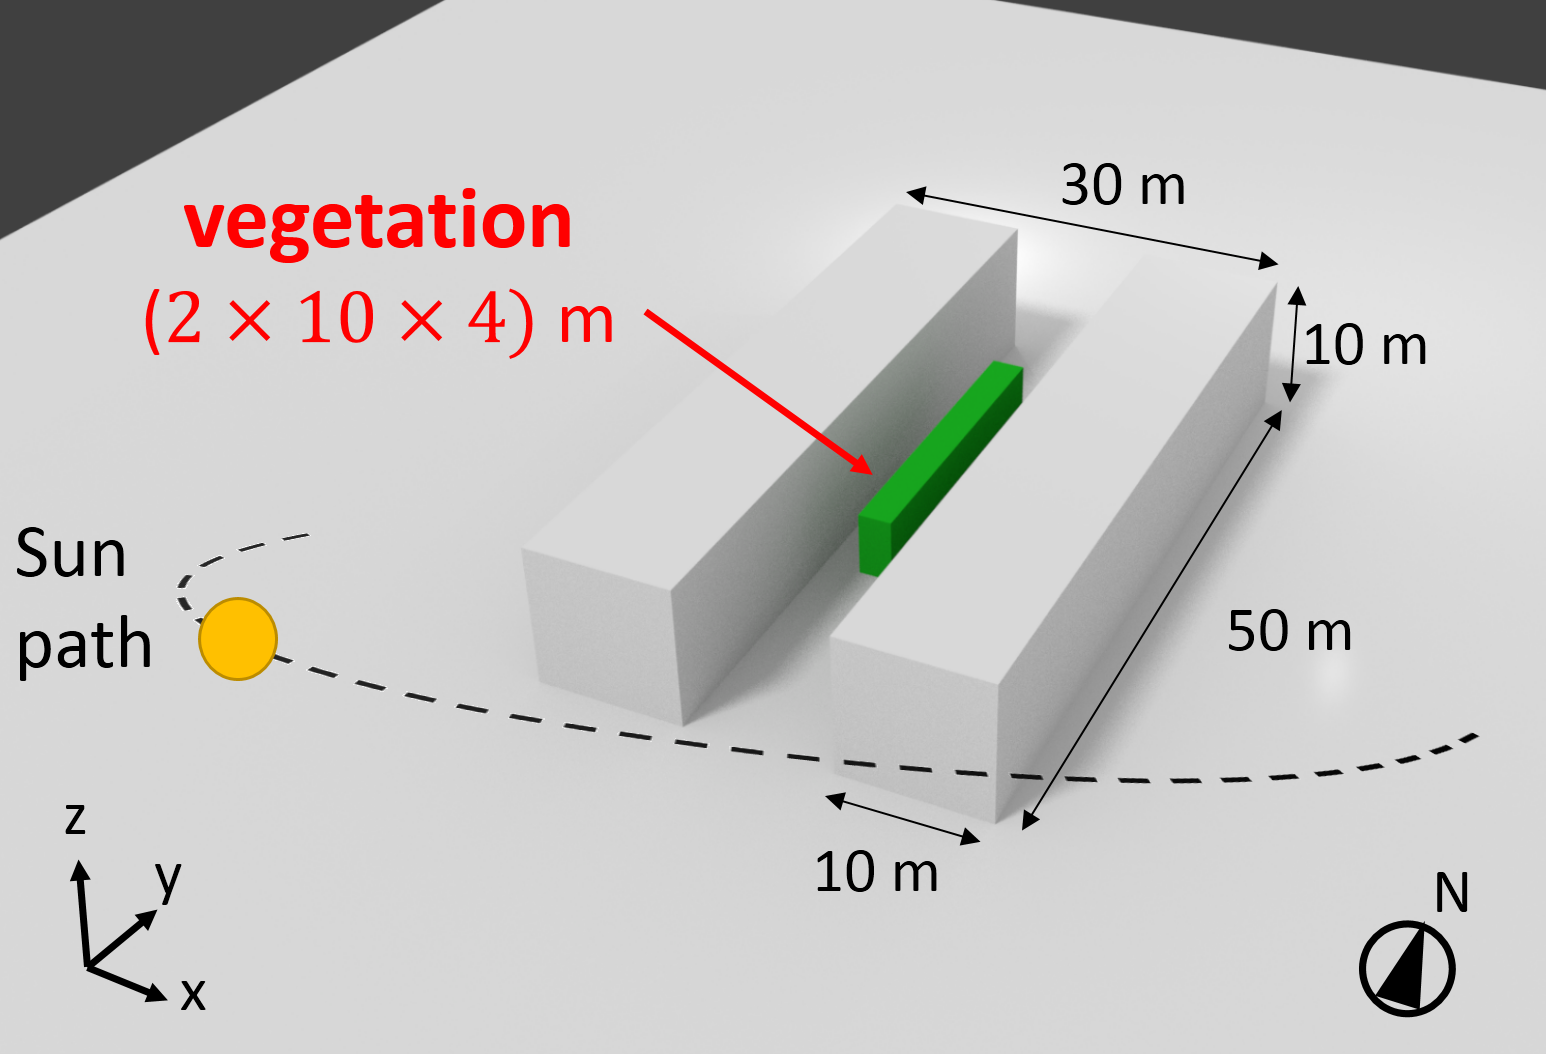
\includegraphics[width=0.8\textwidth]{\figdir/domain_new5.png}
	%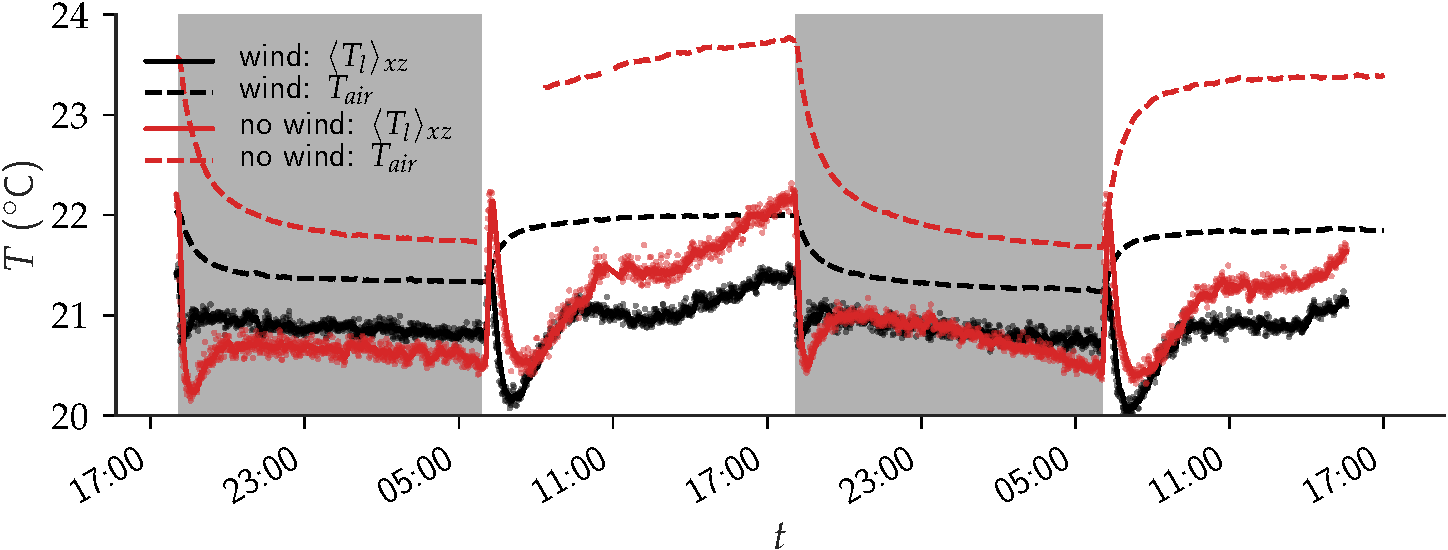
\includegraphics[width=\textwidth]{\figdir/Tinfrared_vs_air_updated-crop.pdf}
	\caption{The simulation setup of a street canyon composed of two buildings measuring $10 \times 50 \times 10$ m$^3$ ($x\times y \times z$) with vegetation band of size $2 \times 10 \times 4$ m$^3$ in the center. The setup is based on the study of \cite{Kubilay2018} awa with wind.}
	\label{fig:domain_new5}
	\end{figure}


\begin{figure}[p]
	\centering
	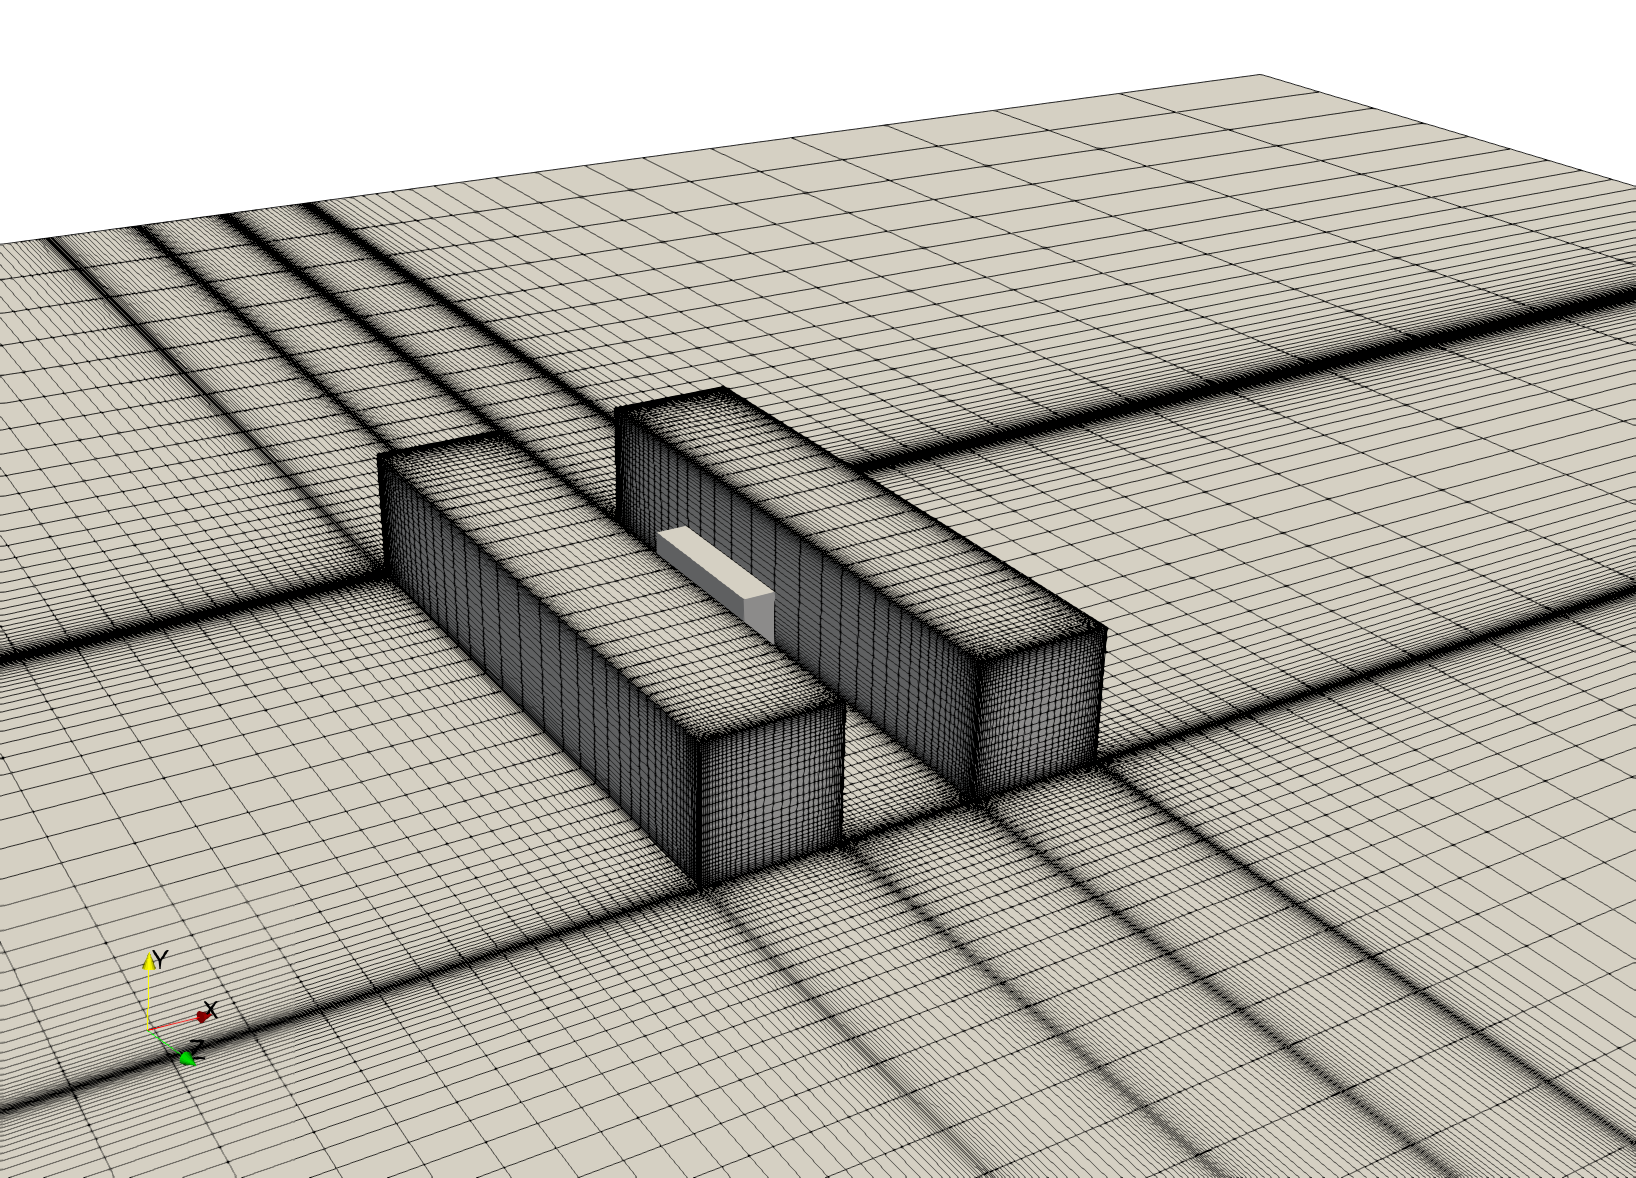
\includegraphics[width=0.6\textwidth]{\figdir/mesh_resolution.png}
	%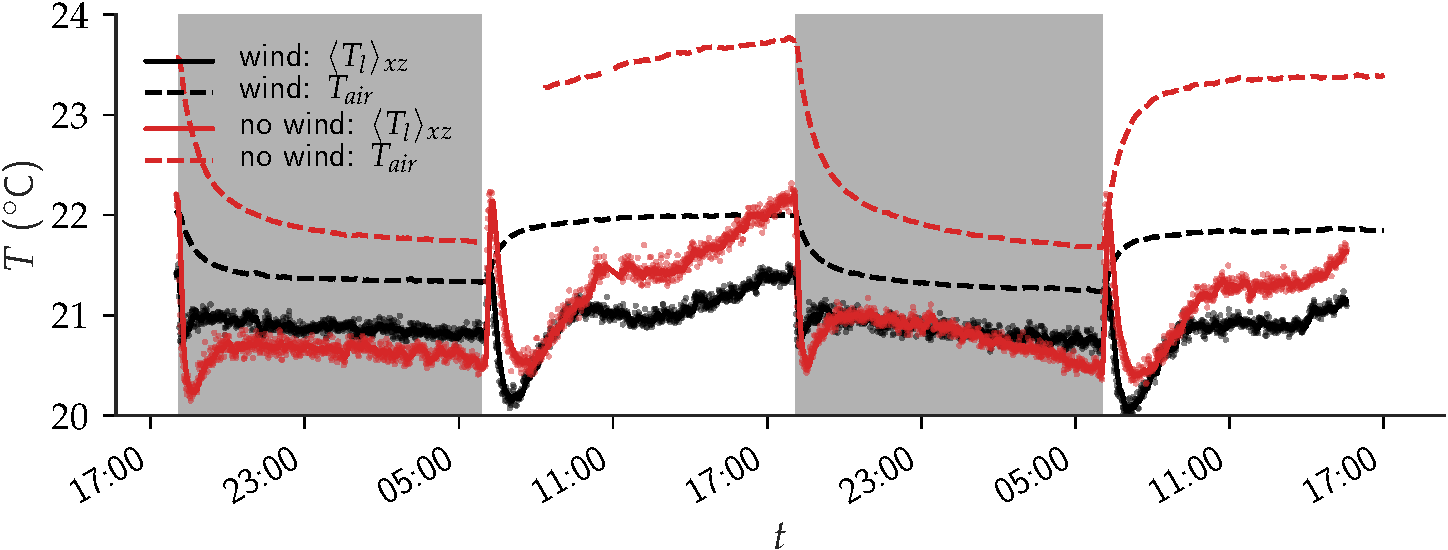
\includegraphics[width=\textwidth]{\figdir/Tinfrared_vs_air_updated-crop.pdf}
	\caption{Simulation domain showing the surface layer mesh refined closed to the building walls. The numerical domain is discretized into $\num{1178080}$ hexahedral cells with minimum cell size of $\num{1e-3}$ m$^{3}$ at the building corner. The mesh is based on the grid refinement study of \cite{Kubilay2018}.}
	\label{fig:mesh_resolution}
\end{figure}

\begin{figure}[p]
	\centering
	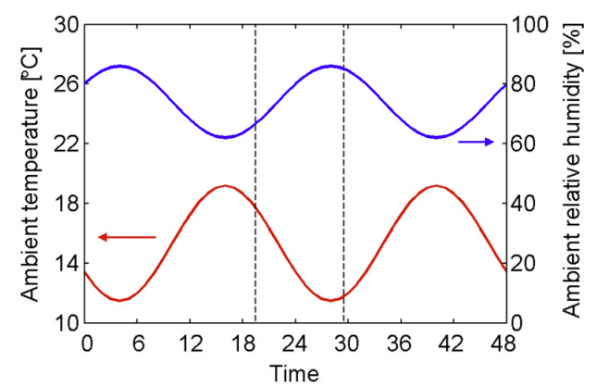
\includegraphics[width=0.8\textwidth]{\figdir/meteobc.png}
	%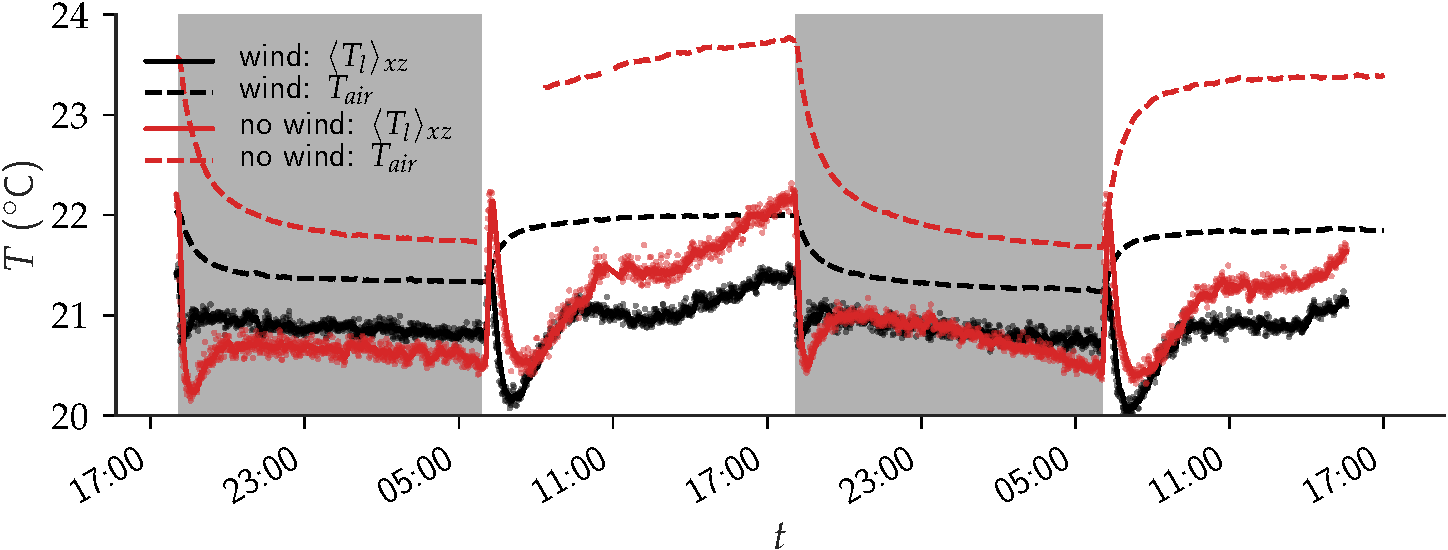
\includegraphics[width=\textwidth]{\figdir/Tinfrared_vs_air_updated-crop.pdf}
	\caption{Diurnal ambient temperature $T$ ($^{\circ}C$) and relative humidity $RH$ (\%) profile obtained from \cite{Kubilay2018}. The meteorological data are based on a typical meteorological year and the total solar radiation intensity is for a clear sky on the 21$^{\mathrm{st}}$ of June in the city of Z\"urich, Switzerland. }
	\label{fig:meteobc}
\end{figure}

\begin{figure}[p]
	\centering
	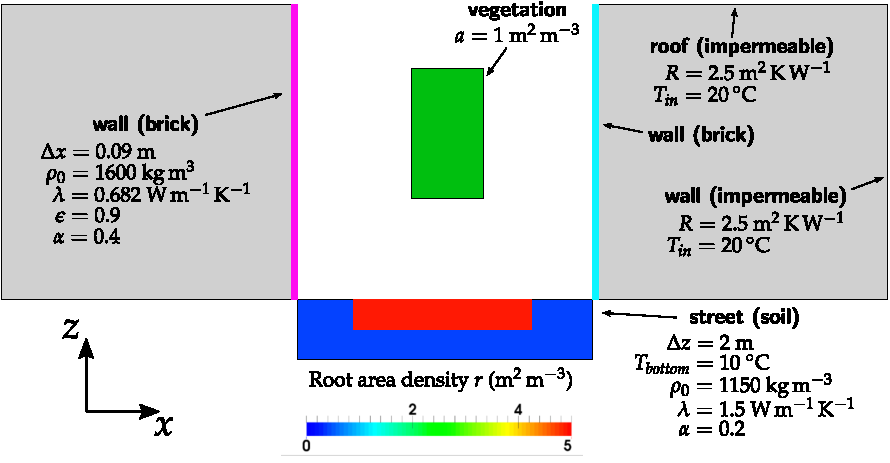
\includegraphics[width=\textwidth]{\figdir/umcconfiguration-crop.pdf}%soliddomain_v2
	%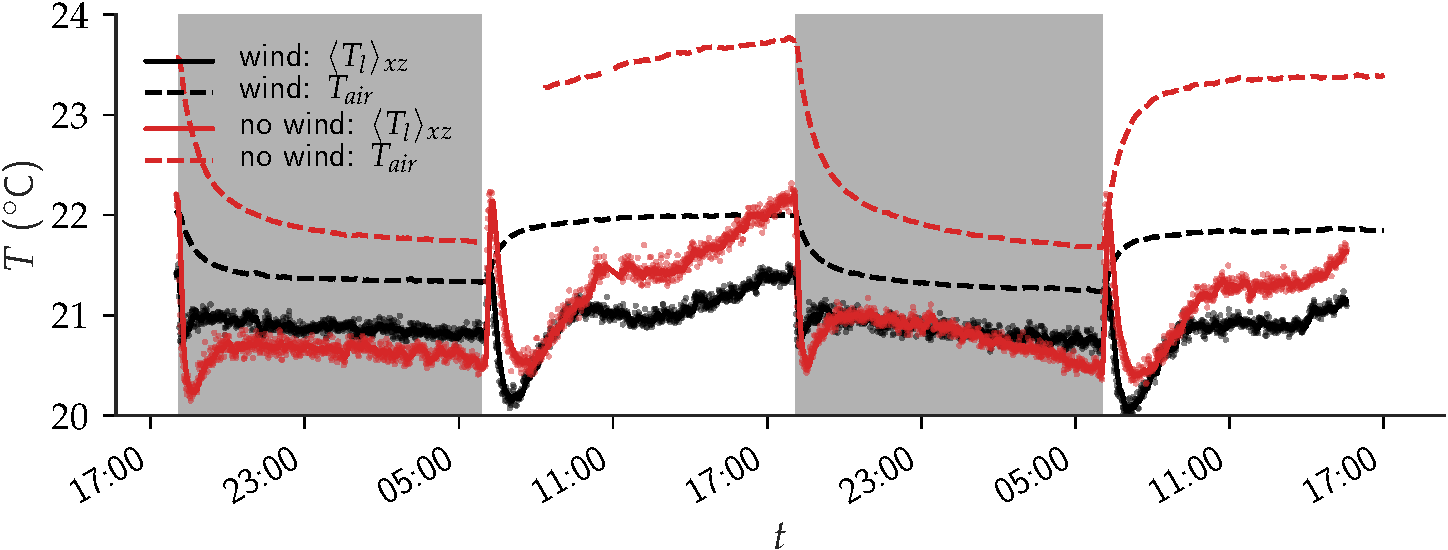
\includegraphics[width=\textwidth]{\figdir/Tinfrared_vs_air_updated-crop.pdf}
	\caption{Description of the solid domain consisting of two impervious buildings of size $10 \times 50 \times 10$ m$^3$ ($x\times y \times z$) each with a brick layer of $0.09$ m inside the street-canyon and a soil region at the street with vegetation roots. The temperature $T_{\textit{in}}$, thermal resistance $R$, the density $\rho_0$, thermal conductivity $\lambda$, emissivity $\epsilon$, albedo $\alpha$, leaf area density $a$ and root area density $r$ and also provided. }
	\label{fig:soliddomain}
\end{figure}


\ctable[
caption = {Soil-plant-atmosphere continuum (SPAC) vegetation parameters of Loblolly pine (\textit{Pinus taeda}) are used in the study \citep{Manoli2014,Volpe2013,Launiainen2015,Manzoni2011,Vogel2016}},
label   = {tab:spacconditions},
pos = p,
mincapwidth = \textwidth,
]{llrl}{}{
	\FL
	Parameter					& Description 				& Value  & Unit
	\ML
	$c$						 	& Ambient CO$_2$ concentration & $380$ & $\mu$mol\,mol$^{-1}$		\\
	$c_*$						 	&  CO$_2$ concentration at max. WUE & $400$ & $\mu$mol\,mol$^{-1}$		\\
	$c_o$						& Ambient O$_2$ concentration & $210$ & mmol\,mol$^{-1}$		\\
	$a$  							& leaf area density		& $1$ &m$^{2}$\,m$^{-3}$\\
	$l$								 & leaf size				 & $0.1$ &m \\	
	
	$\lambda_{\textit{max}}$ & Maximum WUE 	 & $2912$ &$\mu$mol\,mol$^{-1}$	\\
	$\beta_{L}$ &  WUE coefficient & $\num{0.78e-12}$ & \\	
	$\psi_{L}^{\textit{max}}$ &  leaf water potential at max. WUE & $\num{-1.85e-6}$ &Pa\\	
	$k_x$ &  xylem conductance & $\num{5e-6}$ &s$^{-1}$\\	
	$A_x$ &  xylem cross-section area & $0.06$ &m$^{2}$\\
	$k_{\textit{st,n}}$			& nocturnal stomatal conductance & $0.018$ &mol\,m$^{-2}$\,s$^{-1}$ \\	
	$r$ 							 & root area density 	& $5$ &m$^{2}$\,m$^{-3}$	 \\
	$r_{\textit{radius}}$		& root radius 			  & $0.02$ &m \\
	$\beta$						 & soil conductance coefficient & $\num{3e8}$ &\\
	$k_r$							& root conductance 	& $\num{3e-11}$ &s$^{-1}$ \\
	
	\LL}

The coupling of air domain, the solid domains (including soil region), with the vegetation is discussed in \cref{sec:couplingalgorithm}. \cref{fig:soliddomain} shows the setup of the solid domain used in the study. The figure depicts the configuration of two buildings forming a street-canyon with a vegetation zone in the middle. The cross-section is a $x-z$ plane at $y=125$ m  (i.e., $y$-center of the street-canyon). The two buildings have size $10 \times 50 \times 10$ m$^3$ ($x\times y \times z$) each with a brick layer of $0.09$ m inside the street-canyon and a soil region at the street where the vegetation roots is present. The soil is composed of equal composition of sand, silt, and clay with a uniform root area density $r = 5$ m$^{2}$\,m$^{-3}$ of the size of $4 \times 14 \times 1$ m$^{3}$ directly below the foliage region, spanning $\mvec{x}_{\textit{min}} = (62, -1, 118)$ and $\mvec{x}_{\textit{max}} = (68, 0, 132)$. The temperature inside the building $T_{\textit{in}}$, thermal resistance $R$ of wall and roof, the density $\rho_0$, thermal conductivity $\lambda$, emissivity $\epsilon$ and albedo $\alpha$ of the various solid regions are also indicated in \cref{fig:soliddomain}. The vegetation parameters used in the soil-plant-atmosphere continuum (SPAC) vegetation model are given in \cref{tab:spacconditions}. The vegetation properties are for Loblolly pine (\textit{Pinus taeda}) \citep{Manoli2014,Volpe2013,Launiainen2015,Manzoni2011,Vogel2016}. Although not common in cities, this species was used due to the availability of vegetation properties. In future, this numerical modeling approach should enables to study various other species that are more common in cities.

\subsection{Results and Discussion}


The influence of water availability is studied by investigating the evolution of root, leaf, and soil water potentials. We study how the root water uptake changes spatially and diurnally for around 24 days. Such a long time evolution is required to analyze the gradual change in soil moisture. By day 21, the plant is under water stress, and we investigate the impact on the energy balances and the urban microclimate conditions. The influence of vegetation in an urban street-canyon is determined by separately studying the influence of shading and the plant transpiration. The influence of these two parameters on the microclimate inside the street-canyon is studied by determining the influence on air temperature, mean radiation temperature, short-wave radiation intensity, and finally UTCI distribution. 

\subsubsection*{Influence of water availability}

\begin{figure}[p]
	\centering
	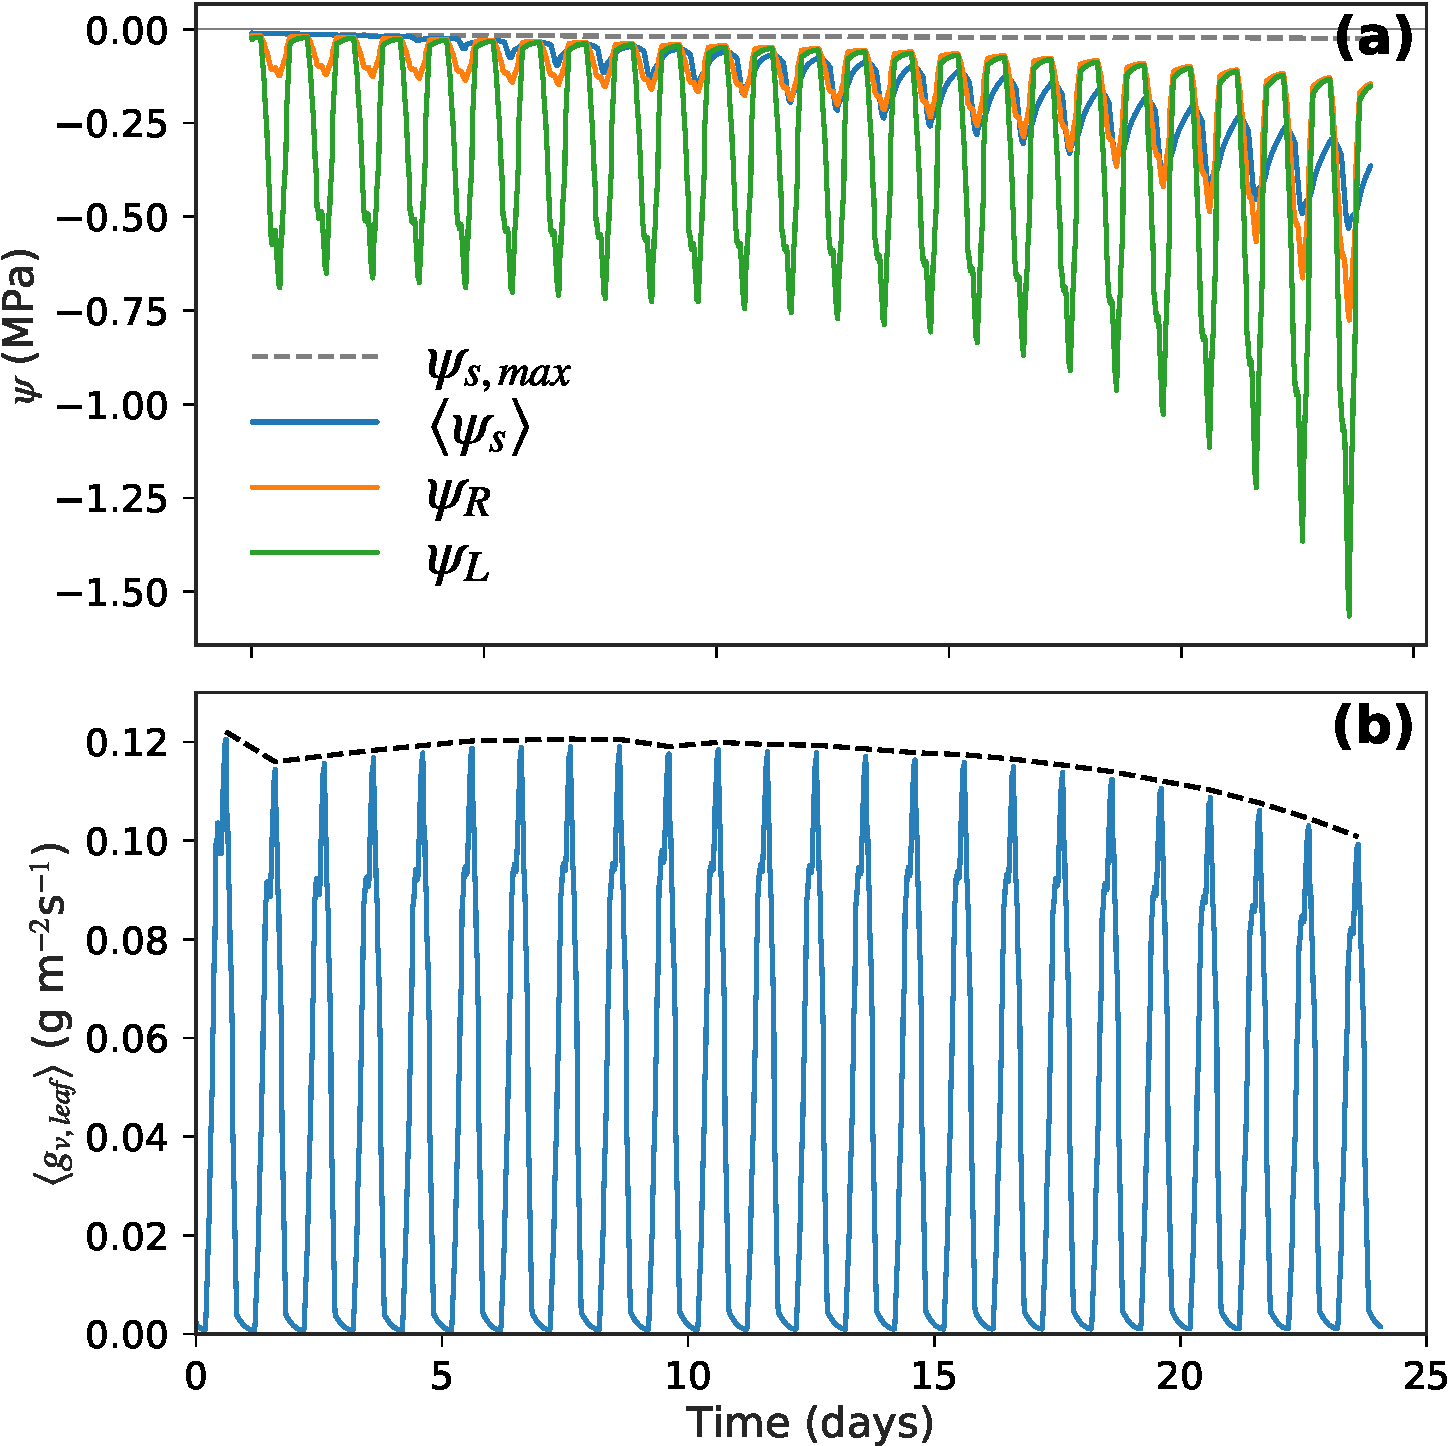
\includegraphics[width=\textwidth]{\figdir/profile_psi_gvleaf_v2-crop.pdf}
	\caption{Long-term evolution of the plant properties changing due reducing water availability, simulated for 24 days: \subfig{a} bulk leaf water potential $\psi_L$ (MPa), bulk root water potential $\psi_R$ (MPa), rhizosphere-averaged soil water potential $\langle \psi_s \rangle$ (MPa) and maximum rhizosphere soil water potential $\psi_{\textit{s,max}}$ (MPa) \subfig{b} average plant transpiration rate $\langle g_{\textit{v,leaf}} \rangle$ (g\,m$^{-2}$\,s$^{-1}$). }
	\label{fig:profile_psi_gvleaf}
\end{figure}

\begin{sidewaysfigure}[p]
	\centering
	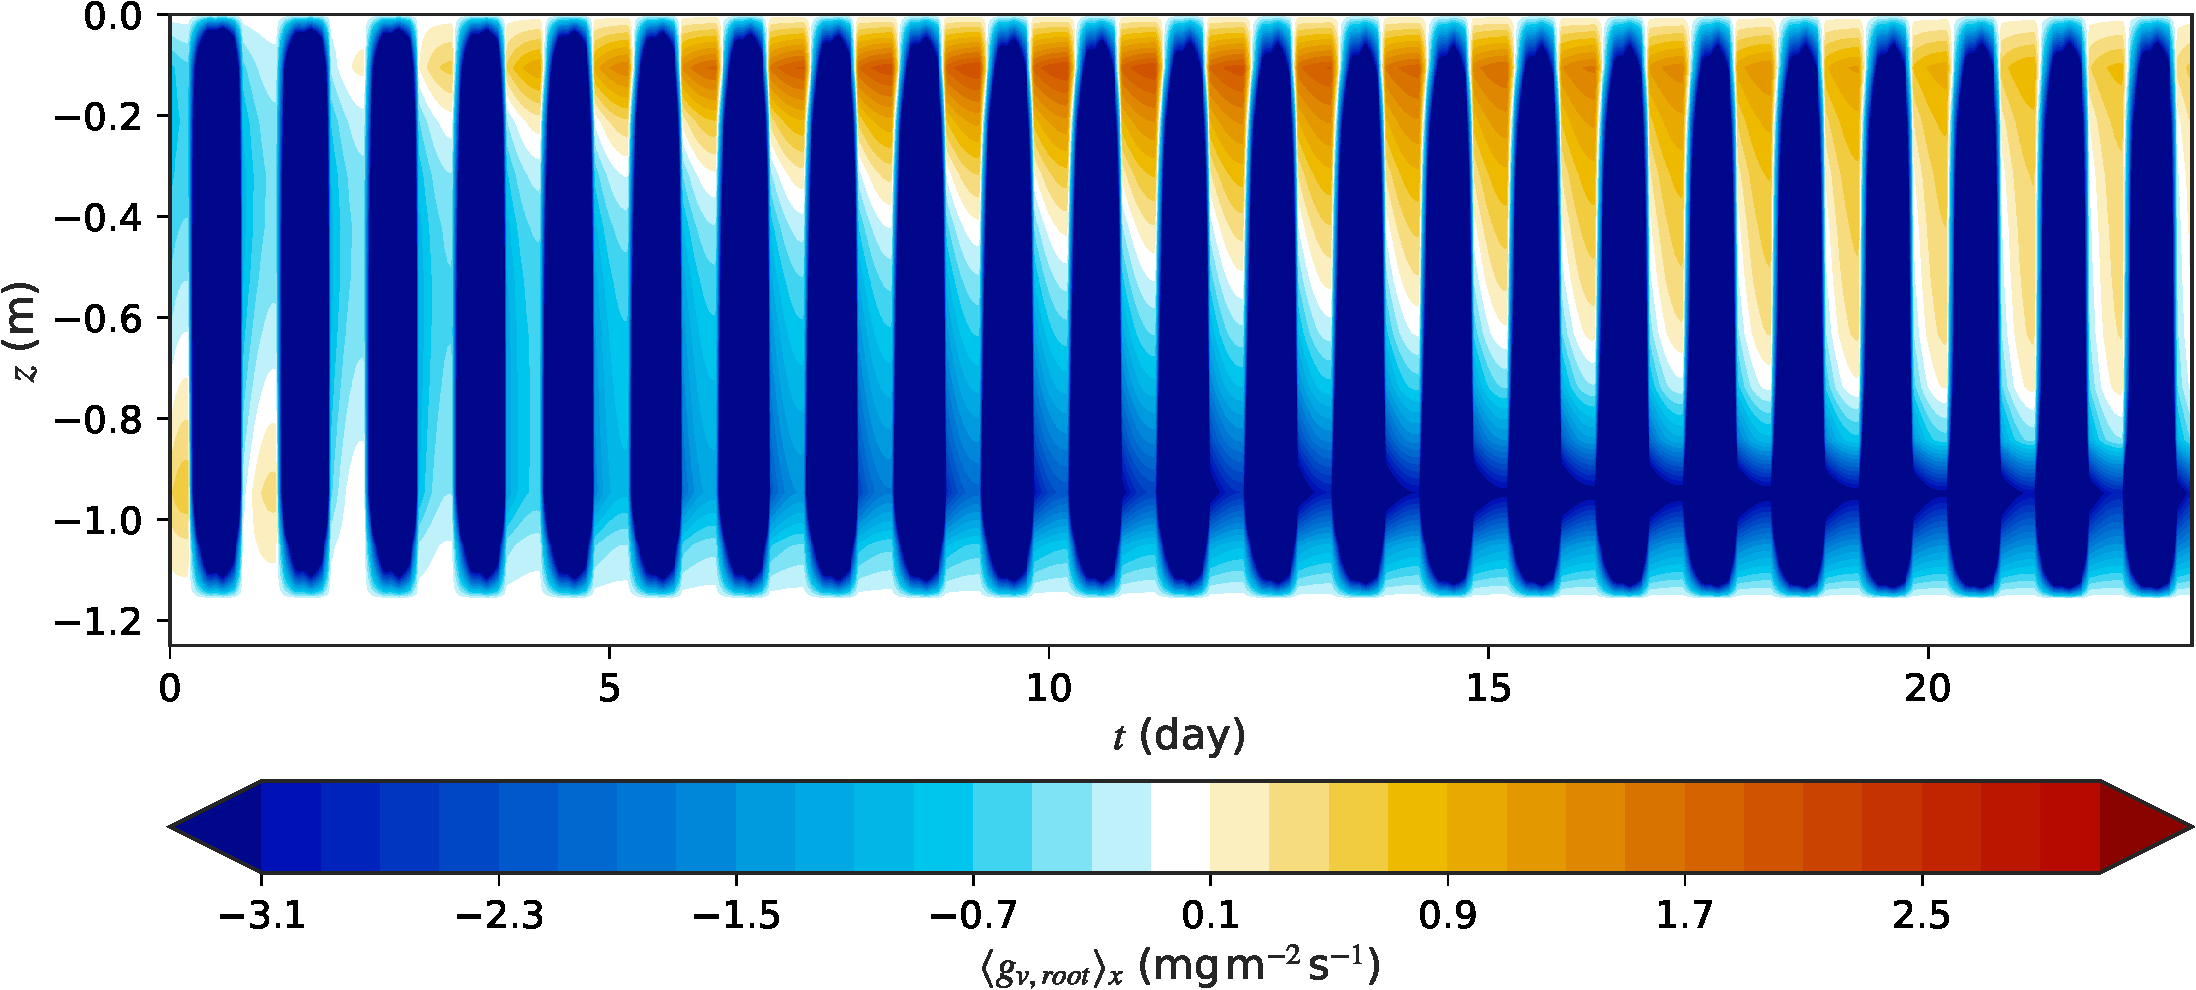
\includegraphics[width=\textwidth]{\figdir/USC_rootwateruptake-crop.pdf}
	\caption{Time evolution of root water uptake vertical distribution $\langle g_{\textit{v,root}} \rangle$ (mg\,m$^{-2}$\,s$^{-1}$) (laterally-averaged). Negative value indicated root uptake from soil to roots and positive value indicates into soil.}
	\label{fig:USC_rootwateruptake}
\end{sidewaysfigure}

\begin{figure}[p]
	\centering
	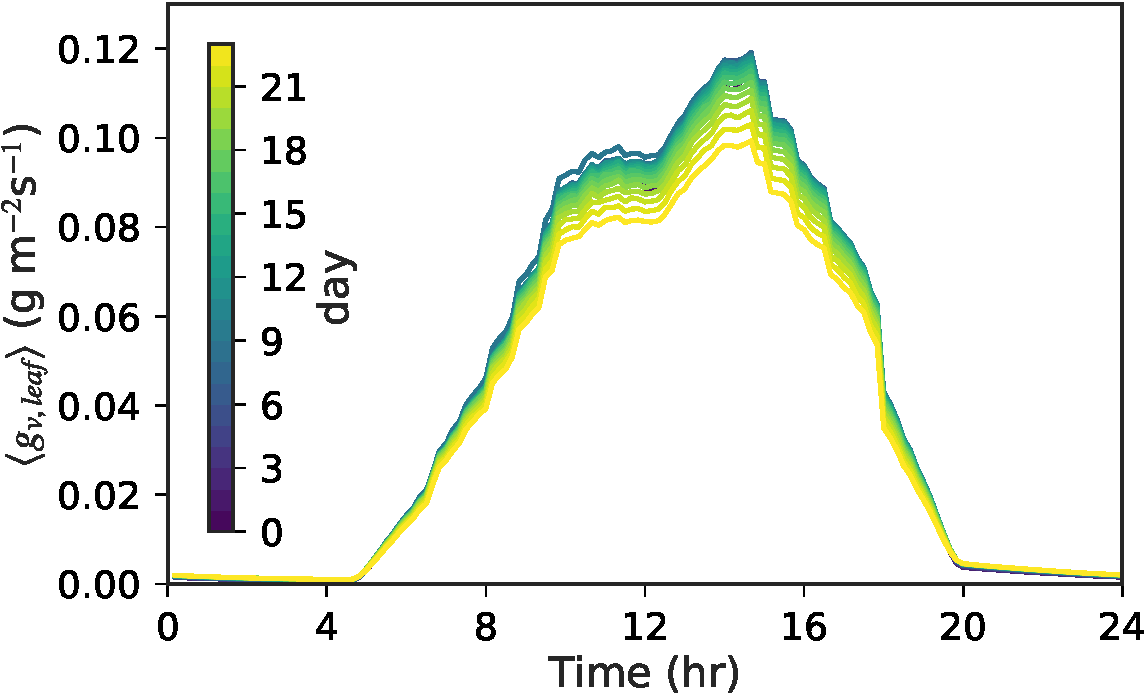
\includegraphics[width=0.8\textwidth]{\figdir/profile_gvleaf_collapsed-crop.pdf}
	\caption{Hourly variation of plant transpiration rate $\langle g_{\textit{v,leaf}} \rangle$ (g\,m$^{-2}$\,s$^{-1}$ for all 24 days.}
	\label{fig:profile_gvleaf_collapsed}
\end{figure}

\begin{figure}[p]
	\centering
	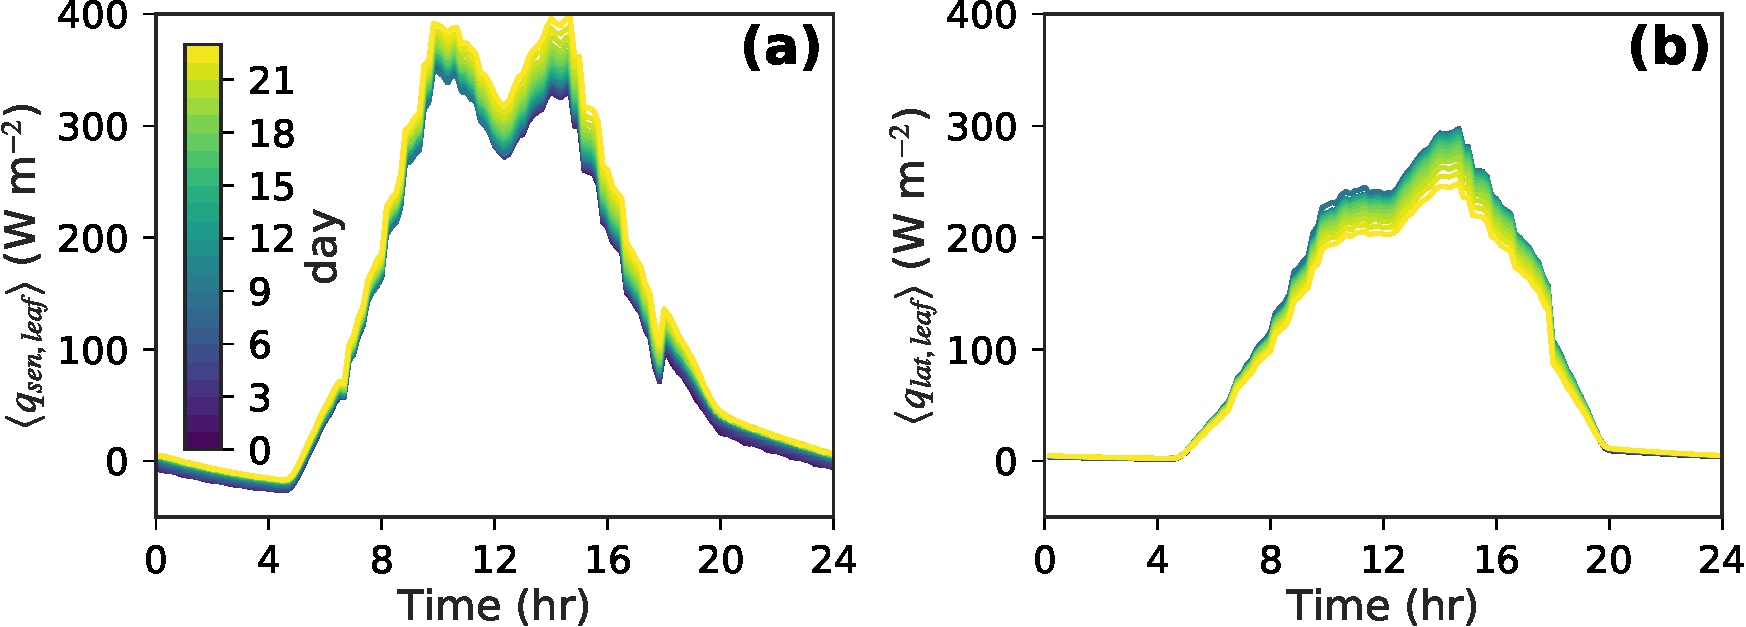
\includegraphics[width=\textwidth]{\figdir/energy_collapsed-crop.pdf}
	\caption{Hourly variation of plant energy fluxes changing due to reducing water availability: \subfig{a} average sensible heat flux $\langle q_{\textit{sen,leaf}} \rangle$ (W\,m$^{-2}$) and \subfig{b} average latent heat flux $\langle q_{\textit{lat,leaf}} \rangle$ (W\,m$^{-2}$). }
	\label{fig:energy_collapsed}
\end{figure}

As the plant transpires throughout the day, the soil moisture will reduce due to the root water uptake (in addition to soil surface evaporation). Therefore, after a longer period (i.e., days), the soil moisture will be reduced and could have an impact on the plant transpiration rate, directly influencing the leaf energy balance. \cref{fig:profile_psi_gvleaf} shows the long-term evolution of the plant properties such as bulk leaf water potential $\psi_L$ (MPa), bulk root water potential $\psi_R$ (MPa), rhizosphere-averaged soil water potential $\langle \psi_s \rangle$ (MPa), and average plant transpiration rate $\langle g_{\textit{v,leaf}} \rangle$ (g\,m$^{-2}$\,s$^{-1}$). The rhizosphere-averaged soil water potential is defined as:
\begin{equation}
\langle \psi_s \rangle = \frac{\int_{\Omega_{\textit{soil}}} r \psi_s~\mathrm{d}V}{\int_{\Omega_{\textit{soil}}} r \mathrm{d}V }
\end{equation}
and average plant transpiration rate is defined as:
\begin{equation}
\langle g_{\textit{v,leaf}} \rangle= \frac{\int_{\Omega_{\textit{air}}} a\, g_{\textit{v,leaf}}~\mathrm{d}V}{\int_{\Omega_{\textit{air}}} a~\mathrm{d}V }
\end{equation}

We see that leaf and root water potential varies at two timescales: i) hourly and ii) daily. The hourly cycling behavior is directly correlated with atmospheric conditions such as solar radiation as depicted in \cref{fig:profile_qsdir_Tmrt}. Around early afternoon (i.e., 15:00), when the solar radiation is highest, the atmospheric evaporative demand (AED) is highest, as experimentally observed in \cref{ch:microclimatestudy}. A large transpiration demand is reflected by the large drop in leaf water potential (\cref{fig:profile_psi_gvleaf}a). Similarly, the root water potential becomes more negative, albeit at a higher than the leaf water potential. The soil water potential follows a similar trend with an even smaller fluctuation between day and night values. However, what is interesting is that the average nocturnal rhizosphere soil water potential is lower than the root water potential. As the night progresses to dawn, we see that soil water potential becomes less negative. It is, therefore, evident that hydraulic redistribution occurs \citep{Volpe2013, Huang2017}. Figure \cref{fig:USC_rootwateruptake} shows the time evolution of root water uptake from the soil for up to 24 days. We see that during day time, there is a strong water uptake from the soil due to leaf transpiration. However, during the night, as the days progress, we observe hydraulic redistribution from the bottom region of the rhizosphere to the surface layer. The rhizosphere region soil moisture is highest just before dawn and is a common metric used in plant science (i.e., pre-dawn soil water potential). The night-time hydraulic redistribution occurs when the soil water potential near the surface is lower than the bulk root water potential. Therefore, the roots act as a mechanism to redistribute the lower-ground water where the water potential is higher (i.e., more saturated), to upper layers of the rhizosphere through the roots. The advantage is that the near-surface soil can be re-moisturized, improving surface evaporative cooling or providing ecological support to ground level vegetation such as grass. The study shows the importance of deep-rooted vegetation which can access the water near the water table and redistribute to regions of driest soil where the soil water potential is lowest.

\cref{fig:profile_psi_gvleaf}b shows the variation in the average plant transpiration rate. The plant transpiration is correlated with the leaf water potential as they are directly dependent, with peak plant transpiration around early afternoon (15:00).  The long-term dynamics of water availability is also visible in the \cref{fig:profile_psi_gvleaf}. As the number of days passes, a larger gradient in the leaf and root water potential is required to provide the adequate transpiration needed by the atmospheric demand. Furthermore, after day 20, we observe an exponential behavior in the daily variability indicating that plants are more susceptible after an extended period of low soil moisture. Furthermore, if we quantify water stress as a difference between the leaf and soil water potential, we see that plant water stress increases exponentially as the day passes. \cref{fig:profile_gvleaf_collapsed} shows the plant transpiration rate $\langle g_{\textit{v,leaf}} \rangle$ (g\,m$^{-2}$\,s$^{-1}$), where all the 24 days are collapsed to an hourly plot. We see that with an increasing number of days without irrigation, the plant transpiration decays throughout the day and is proportional to the level of the plant transpiration. The largest drop in plant transpiration is observed at peak solar hour.

To understand how the decaying transpiration rate affects the plant energy balance, the hourly variation of the average sensible heat flux $\langle q_{\textit{sen,leaf}} \rangle$ (W\,m$^{-2}$) and  average latent heat flux $\langle q_{\textit{lat,leaf}} \rangle$ (W\,m$^{-2}$) is investigated, \cref{fig:energy_collapsed}. The figure shows that with reducing water availability, the sensible heat flux increases throughout the day with an equal reduction in the latent heat flux.  This results in the diminished cooling provided by the vegetation, as observed in \cref{fig:profile_T_UTCI}. The study shows the importance of the regular irrigation of the vegetation. Without adequate irrigation, a lack of water for plant transpiration can remove the transpirative cooling effect observed in \cref{fig:profile_T_UTCI}. If the amount of water in the soil reaches $\psi = \num{-1.5e6}$ (Pa), it is known as the permanent wilting point (PWP) where plants can no longer transpire due to loss of cell turgidity \citep{Idso1977}. So, to ensure the health of the plant, it is important that plants are regularly irrigated. The study shows that, with an increasing number of days (for the previous irrigation), the need for irrigation grows exponentially, reflected by the increasing water stress.


\subsubsection*{Influence of plant transpiration and shading}

\cref{fig:USC_qrdir} shows the direct short-wave radiation intensity $q_{\textit{s,dir}}$ (W\,m$^{-2}$) inside the street-canyon (i.e., $x-z$ plane at $y=125$ m) where the vegetation zone is indicated by a green box. Nine subplots are shown of different times of the days from 03:00 to 23:00 (HH:MM) at 150 minutes interval. The figure shows the contribution of the vegetation to the solar radiation intensity inside the street-canyon. We see that vegetation intercepts the solar radiation during the day providing shading to the nearby urban surfaces. The vegetation acts as a radiation sink especially when the solar radiation is high during noon. It is important as the urban materials with high thermal capacity contribute to the urban heat island by absorbing the solar radiation. By providing shading to the urban environment, vegetation can, therefore, reduce the urban heat island effect.  

\begin{sidewaysfigure}[p]
	\centering
	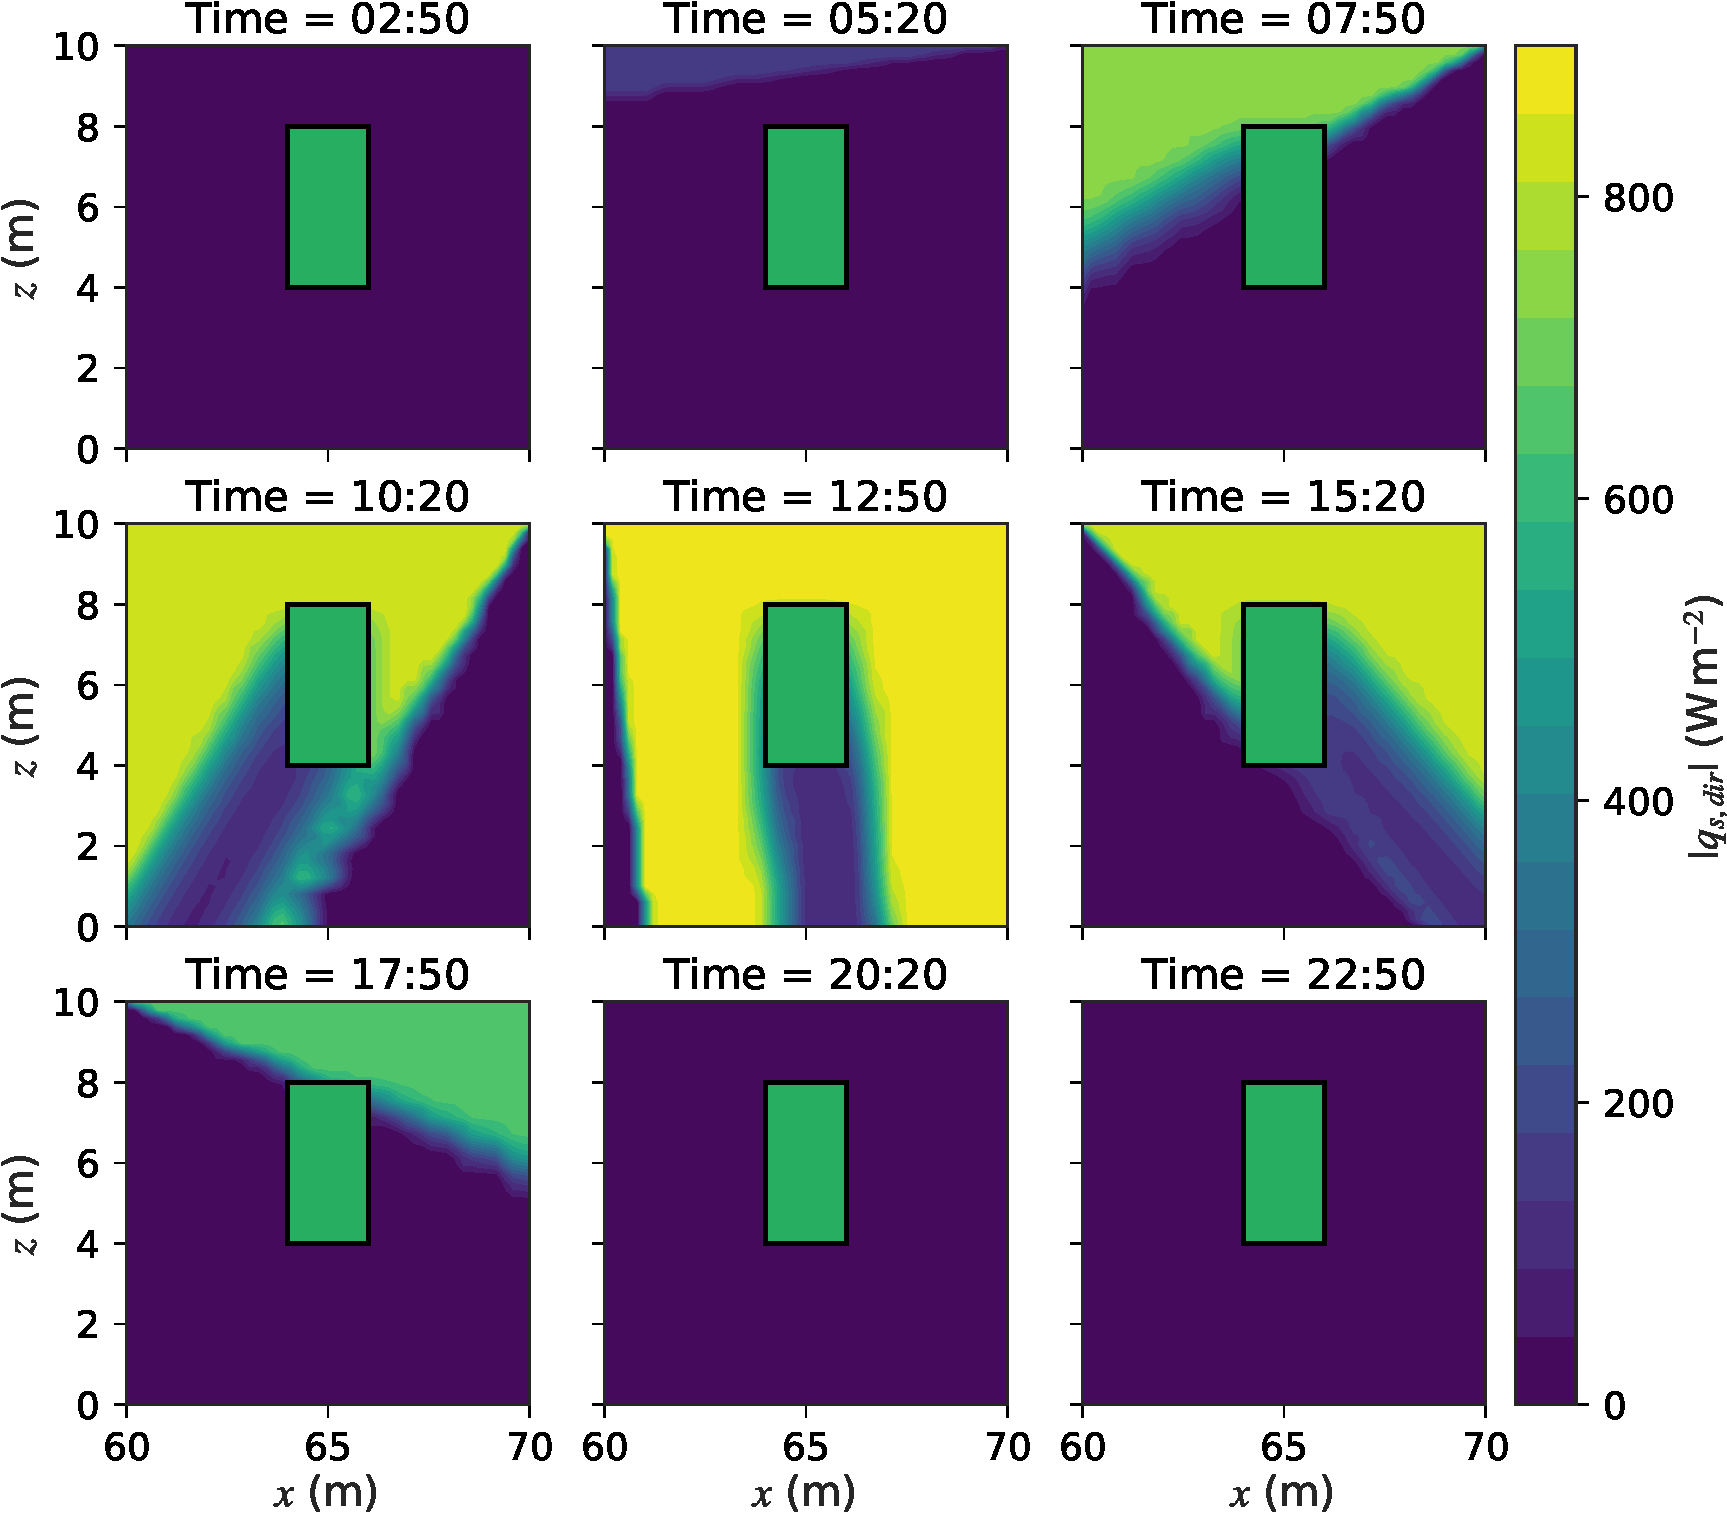
\includegraphics[width=0.8\textwidth]{\figdir/USC_qsdir_type2-crop.pdf}
	\caption{Direct short-wave radiation intensity $|q_{\textit{s,dir}}|$ (W\,m$^{-2}$) inside the street-canyon where the vegetation zone is indicated by a green box. The plot shows the fields with a 150 minutes interval from 03:00 to 23:00 (HH:MM).}
	\label{fig:USC_qrdir}
\end{sidewaysfigure}

\begin{sidewaysfigure}[p]
	\centering
	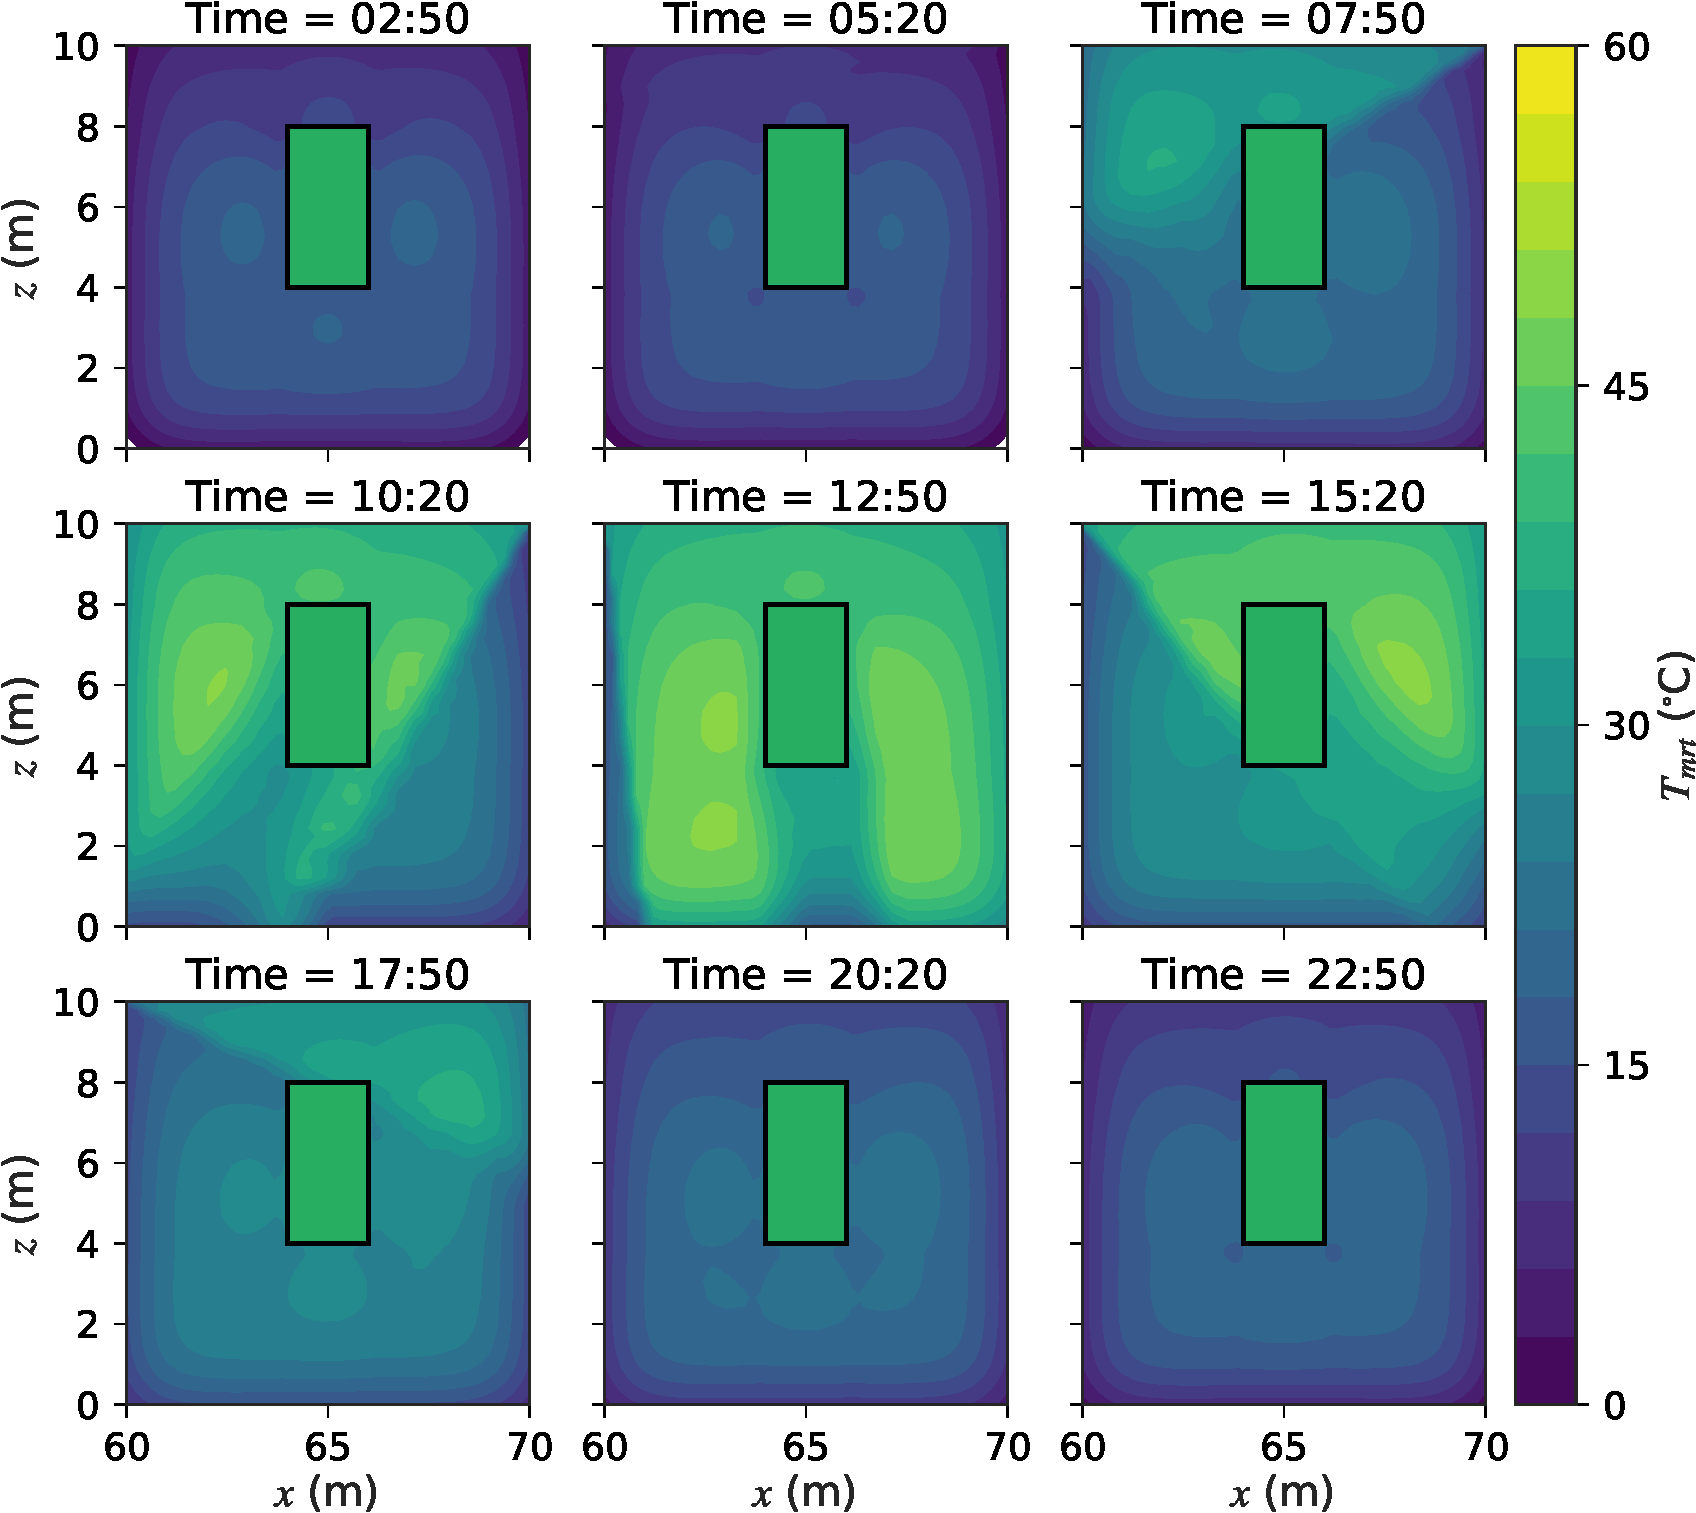
\includegraphics[width=0.8\textwidth]{\figdir/USC_Tmrt_type2-crop.pdf}
	\caption{Mean radiant temperature $T_{\textit{mrt}}$  ($^{\circ}$C) inside the street-canyon where the vegetation zone is indicated by a green box. The plot shows the fields with a 150 minutes interval from 03:00 to 23:00 (HH:MM).}
	\label{fig:USC_Tmrt}
\end{sidewaysfigure}



\cref{fig:USC_Tmrt} shows the mean radiant temperature $T_{\textit{mrt}}$  ($^{\circ}$C) inside the street-canyon throughout the day that a person would experience. Although $T_{\textit{mrt}}$ is a surface related value, in this study we calculate $T_{\textit{mrt}}$ everywhere in the street-canyon to determine how UTCI felt by a person is varying inside the street-canyon. The goal is to have a better understanding of the driving factors behind the thermal comfort and how they are interrelated. The mean radiant temperature is determined as follows: 
\begin{equation}
T_{\textit{mrt}} = \left( T_{\textit{umrt}}^4  + \frac{f_p a_b}{\epsilon_p \sigma} q_{\textit{s,dir}} \right)^{\frac{1}{4}}
\label{eq:Tmrt2}
\end{equation}
where $T_{\textit{umrt}}$ is the mean radiant temperature component belonging to the diffused or reflected part (i.e., from terrestrial source), $f_p$ is projected surface area of the person exposed to the sun, $\alpha_p$ is the albedo, $\epsilon_p$ is the emission coefficient and $q_{\textit{s,dir}}$ (W\,m$^{-2}$) is the direct solar radiation. The diffused/reflected component of the MRT is defined as:
\begin{equation}
T_{\textit{umrt}} = \left[ \frac{1}{\sigma} \sum_{i}^N \left(q_{\textit{r,i}} + \frac{a_b}{\epsilon_p} q_{\textit{s,i}} \right)F_i\right]^{\frac{1}{4}}
\label{eq:Tumrt2}
\end{equation}
where $q_{\textit{r,i}}$ (W\,m$^{-2}$)  is the long-wave radiation emitted from surface $i$, $q_{\textit{s,i}}$ (W\,m$^{-2}$) is the reflected (assumed to be diffused) short-wave radiation from surface $i$, and $F_i$ is the view-factor between surface $i$ and the person. Thus, the mean radiant temperature $T_{\textit{mrt}}$ is directly dependent on the long-wave and the short-wave radiation fluxes in the street-canyon, including the contribution from the direct solar radiation $q_{\textit{r,dir}}$. \cref{fig:USC_Tmrt} is seen to be directly correlated with the short-wave radiation plots depicted in \cref{fig:USC_qrdir}. At regions of high direct solar radiation, the mean radiant temperature approaches $T_{\textit{mrt}}\rightarrow60$ ($^{\circ}$C). In the shaded regions, there is an $18$  ($^{\circ}$C) difference in the mean radiant temperature. This indicates that solar radiation plays a crucial role in the mean radiant temperature and thereby the thermal comfort (investigated in detail in the next section). Furthermore, we see that between the vegetation and the buildings, the mean radiant temperature is at the highest. This is related to the emitted (or reflected) radiation from urban surfaces. At these locations, the region is exposed to (or ``views'') more surfaces emitting and reflecting the radiation. Therefore, the diffused radiation from the building surfaces is also contributing to the mean radiant temperature. During night-time, we see that the mean radiant temperature gradually reduces. This is due to the nocturnal radiation cooling, where the long-wave radiation from the building surfaces is emitted to the atmosphere during the night, thereby cooling the building surfaces. Trapping of this radiation such as due to cloud cover or even the presence of vegetation can negatively affect the nocturnal radiation cooling.


% In the vicinity of the vegetation, a localized small cooler region is present and is due to the air temperature cooling from plant transpiration. The transpirative cooling is predominant from mid-day to afternoon (i.e., 13:00 to 18:00) when the solar radiation is present and so provides cooling when radiation intensity is highest. 
To better investigate the impact of plant shading and the changes in mean radiant temperature in the street-canyon due to vegetation, a single point below the vegetation at $(x,y,z) = (65, 125, 2)$ is investigated for three different cases: the configuration without vegetation (\textit{None}), a configuration with vegetation but providing only shading (\textit{Shad.}), and a configuration with vegetation providing both shading and plant transpiration (\textit{TR + Shad.}), \cref{fig:profile_qsdir_Tmrt}. \cref{fig:profile_qsdir_Tmrt}a shows the diurnal variation of the direct short-wave radiation intensity $q_{\textit{s,dir}}$ (W\,m$^{-2}$) below the vegetation. At the presence of vegetation, we see a strong drop in the solar radiation, especially during middays from $q_{dir} \approx 800$ W\,m$^{-2}$ to around $100$ W\,m$^{-2}$ at midday. The diurnal profile of the mean radiant temperature $T_{\textit{mrt}}$ ($^{\circ}$C), \cref{fig:profile_qsdir_Tmrt}b, shows that shading provides up to $\approx 20$ $^{\circ}$C drop when shaded and transpiring. This is especially beneficial as the largest temperature drop is found at the time of the highest solar radiation. Thus, shading can be a vital component in improving pedestrian thermal comfort. A detailed investigation of the impact of shading on UTCI is performed in the next section. At night we see that the vegetation instead increases the mean radiant temperature inside the street-canyon. This occurs because vegetation results in a radiation trapping intercepting the long-wave radiation emitted from the urban surfaces to the sky. This phenomenon can, therefore, harm thermal comfort during night time. There is a slight difference between the shaded only case and transpiring case, due the cooler air temperature from transpirative cooling (see \cref{fig:profile_qsdir_Tmrt}c). The reduced air temperature results in a reduced surface temperatures, providing a lower long-wave radiation emissions.

\begin{figure}[p]
	\centering
	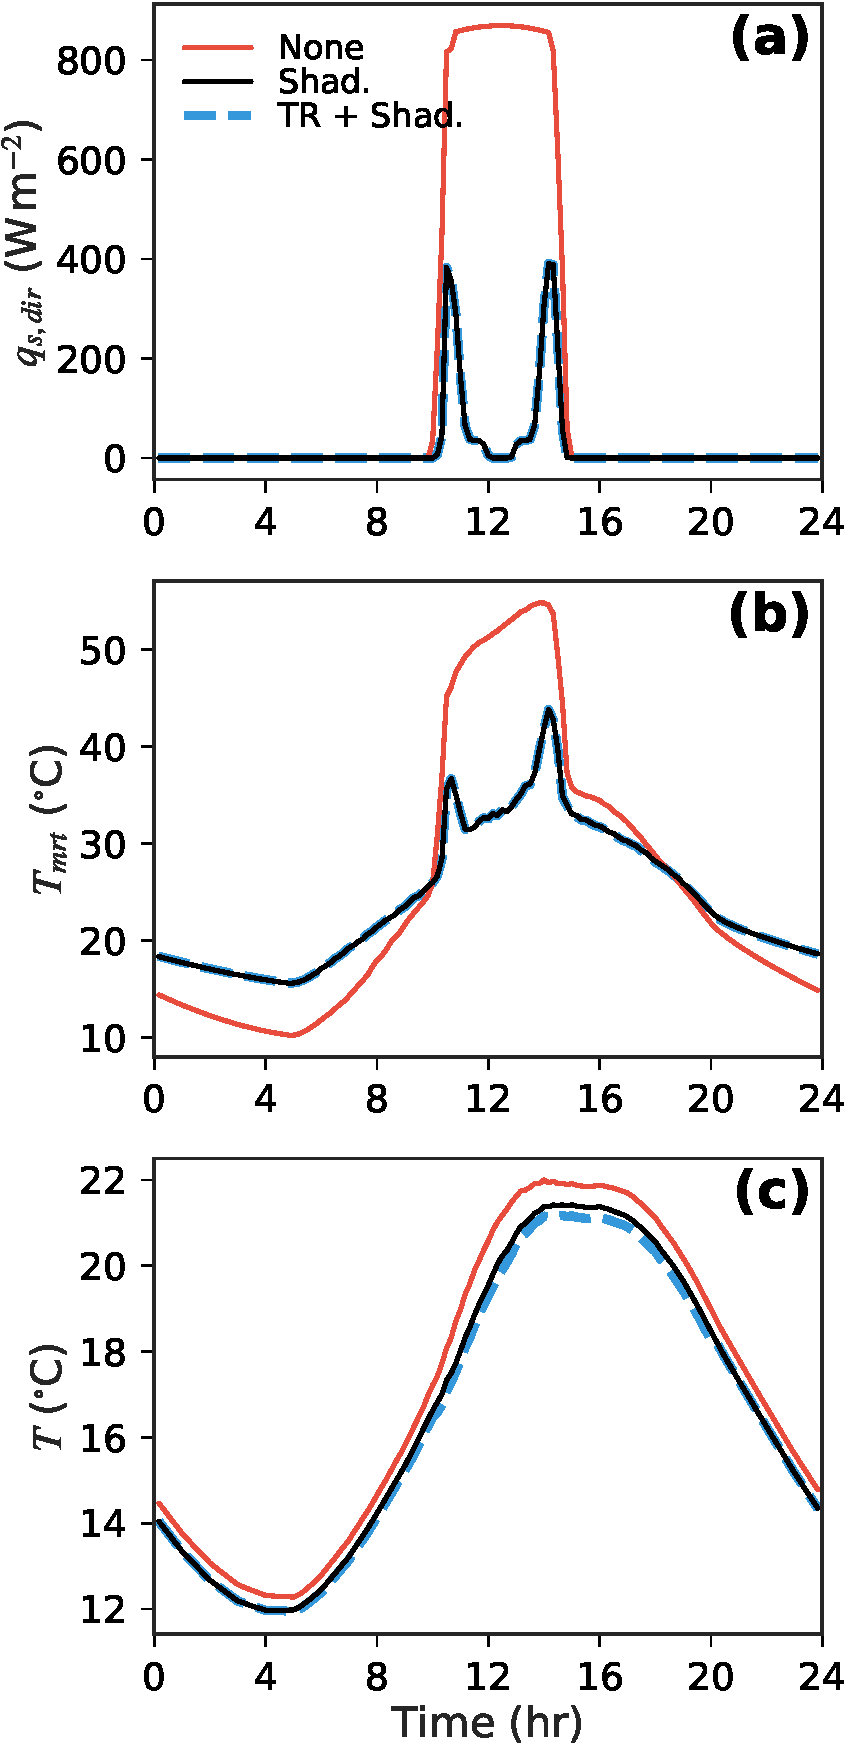
\includegraphics[height=0.8\textheight]{\figdir/profile_qsdir_Tmrt_type3-crop.pdf}
	\caption{Diurnal profile below the vegetation at $(x,y,z) = (65, 125, 2)$ comparing three cases: no vegetation (\textit{None}), vegetation with only shading (\textit{Shad.}), and vegetation providing shading and transpirative cooling (\textit{TR + Shad.}): \subfig{a} direct short-wave radiation intensity $q_{\textit{s,dir}}$ (W\,m$^{-2}$), \subfig{b} mean radiant temperature $T_{\textit{mrt}}$  ($^{\circ}$C), and \subfig{c} air temperature $T$  ($^{\circ}$C).}
	\label{fig:profile_qsdir_Tmrt}
\end{figure}

\begin{sidewaysfigure}[p]
	\centering
	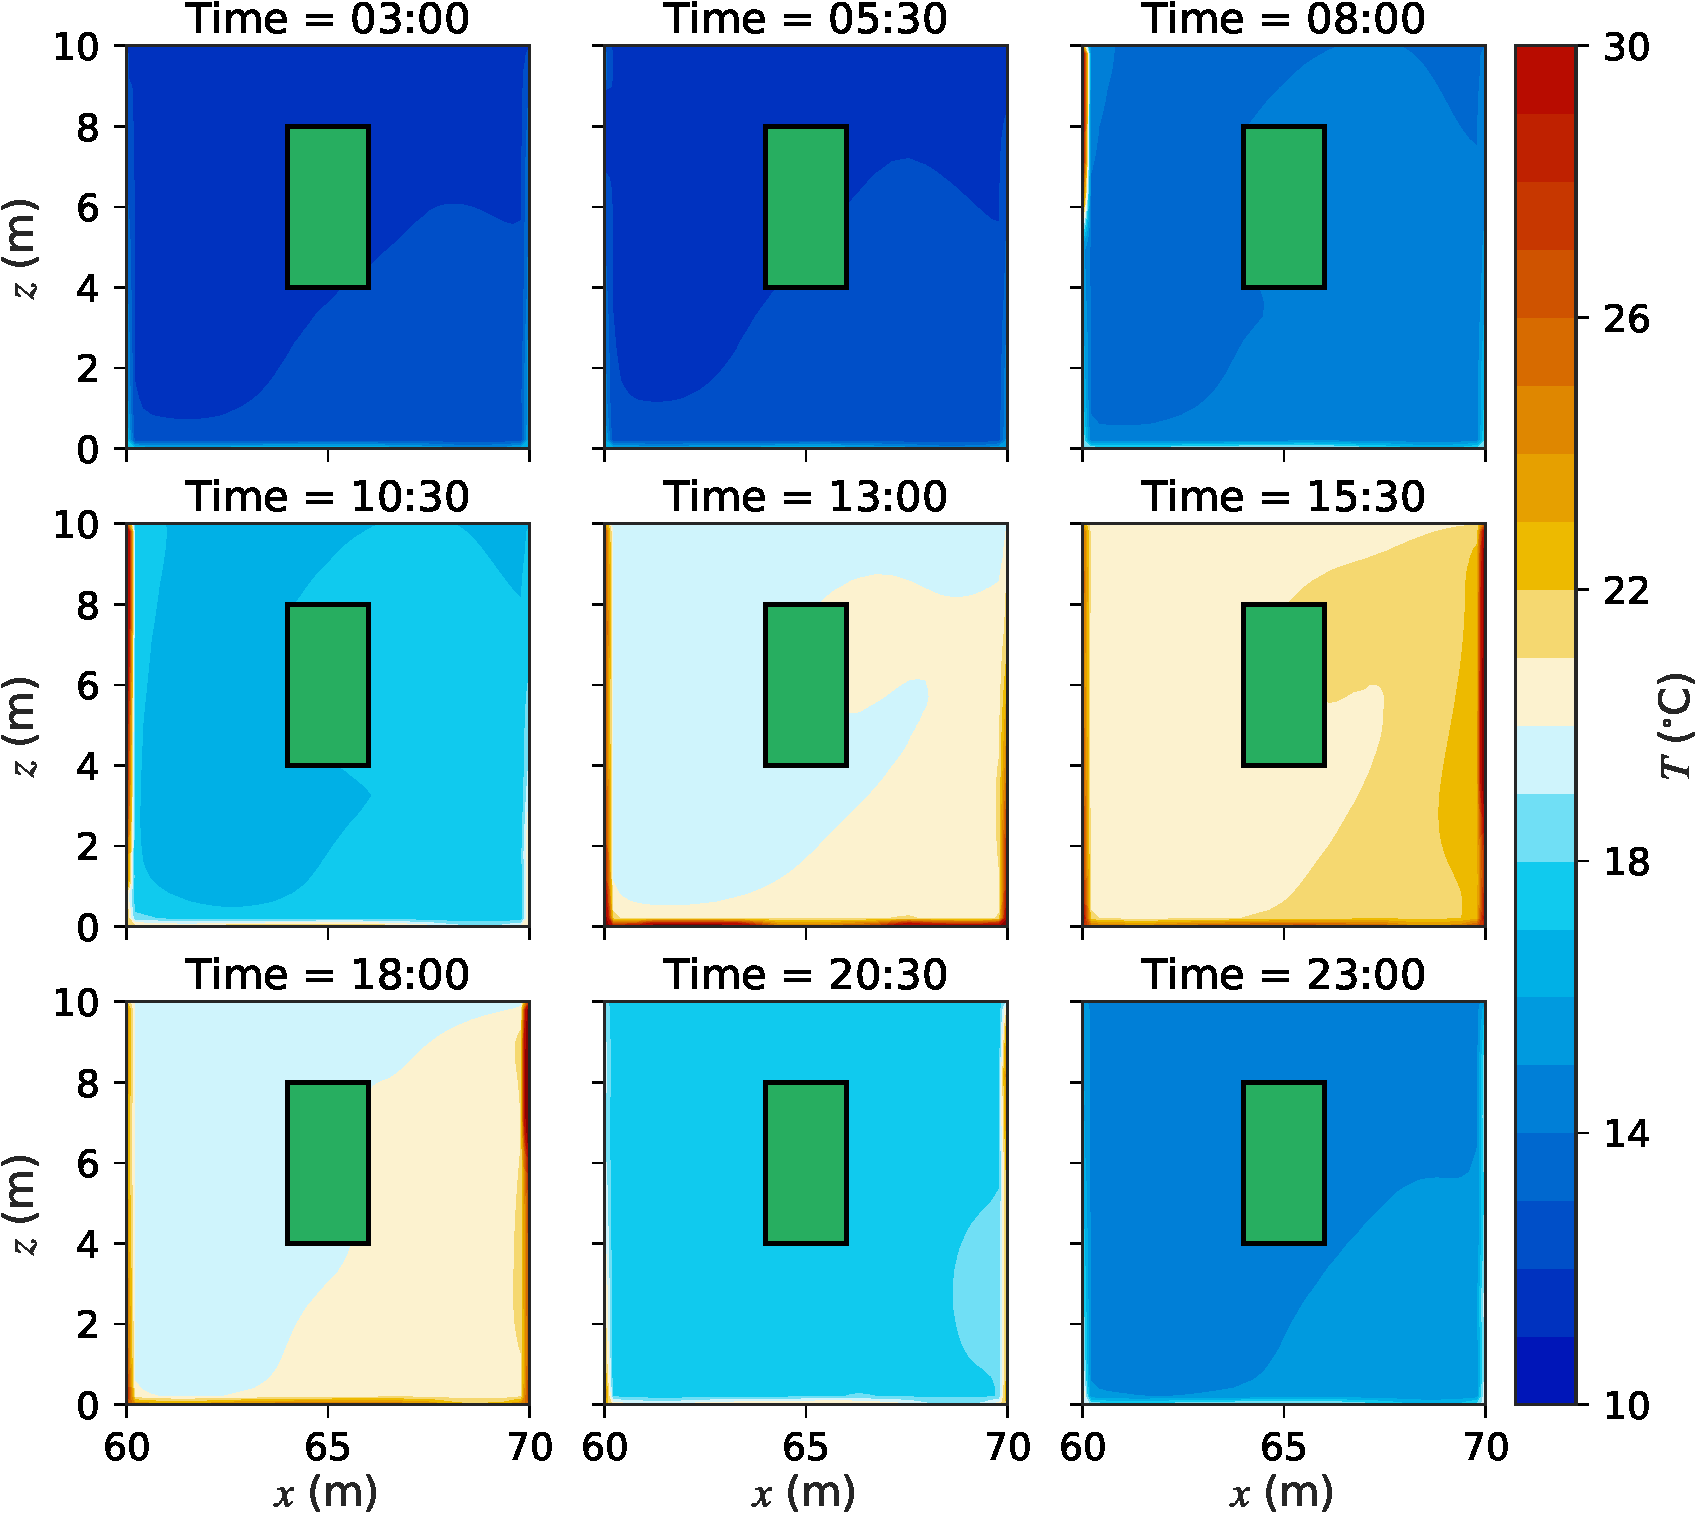
\includegraphics[width=0.8\textwidth]{\figdir/USC_T_type2_v2-crop.pdf}
	\caption{Air temperature $T$ ($^{\circ}$C) inside the street-canyon where the vegetation zone is indicated by a green box. The plot shows the fields with a 150 minutes interval from 03:00 to 23:00 (HH:MM).}
	\label{fig:USC_T}
\end{sidewaysfigure}

\cref{fig:USC_T} shows the air temperature $T$ ($^{\circ}$C) inside the street-canyon (i.e., $x-z$ plane at $y=125$ m) allowing to see the influence of vegetation on the air temperature through the diurnal cycle. The air temperature $T$ depicted in the figures results from the net effect of solar radiation, plant shading, thermal storage in buildings and air temperature change due to plant transpiration. It is apparent that the highest air temperature is at building surfaces mainly due to the solar radiation observed in \cref{fig:USC_qrdir}. Below the vegetation, we see that the air temperature is lower whereas a slight rise in air temperature is observed at the top of the foliage, where most of the solar radiation is intercepted. To better assess the influence of the transpiration and the influence of shading, the air temperature $T$ ($^{\circ}$C) and $UTCI$  ($^{\circ}$C) below the vegetation at $(x,y) = (65, 125)$ and at three different heights $z = [1,2,3]$ are investigated. We compare various cases: i) no vegetation, ii) only shading at day 1, iii) shading and plant transpiration at day 1, and iv) shading and plant transpiration at day 21 (i.e., 20 days after initial irrigation). The last case focuses on the impact of water stress on the cooling provided by vegetation. \cref{fig:profile_T_UTCI}(a-b) show the diurnal variation of the air temperature and the comfort index at $z=2$ m, respectively. \cref{fig:profile_T_UTCI}(c-d) show the difference between \textit{with} and \textit{without} vegetation case (i.e., $\phi_{\textit{case,i}} - \phi_{\textit{none}}$) at the three different heights. It is found that on the first day, for both cases of with both transpiration and shading, and with only shading, there is a significant reduction in the air temperature, especially during the afternoon. On day 1 with the addition of transpiration (i.e., \textit{TR + Shad. - day 1}), we notice an additional cooling that persists till night. We see that after a long period without irrigation (i.e., 20 days), the plant cooling diminishes to the case similar to \textit{without} vegetation. It is possibly due to additional heating up by convective air flow arising from the now present heated up tree with reduced water availability. \cref{fig:profile_T_UTCI}c shows the difference in air temperature \textit{with} and \textit{without} vegetation at three different heights $z=[1,2,3]$. We observe that most cooling is obtained on day 1 with transpiration and shading (i.e., \textit{TR + Shad. - day 1}) at the height $z=1$ m. Away from the ground, the cooling is seen to reduce. So, the strongest cooling is present closer to the ground surface at midday due to cooling from shading and surface evaporation of plant soil. After 20 days, we see that cooling is substantially lower, and the air temperature is even higher during the night. This shows that with water stress in combination with radiation trapping could have negative consequences on the urban microclimate. Due to the lack of transpirative cooling and reduced night-time long-wave radiation escape, the street-canyon air temperature becomes higher over time. The implication of this on thermal comfort on various cases is studied in the next section.
	
	
%The calculated \textit{UTCI} shows that the comfort perceived by the pedestrian \textit{with} and \textit{without} transpiration is identical. 
%
%The perceived change in comfort is simply due to the change in radiative exchanges, influenced by the vegetation. 
%
%So, the change in the mean radiant temperature, seen in \cref{fig:profile_qsdir_Tmrt}, plays a more important role in thermal comfort. 
%
%During night time, the UTCI with vegetation is slightly higher and is due to the higher mean radiant temperature observed in \cref{fig:profile_qsdir_Tmrt}. 
%
%Due to the radiation trapping, the nocturnal UTCI is higher can, therefore, indicate a lower thermal comfort. 


\subsubsection*{Impact on thermal comfort}

\begin{figure}[p]
	\centering
	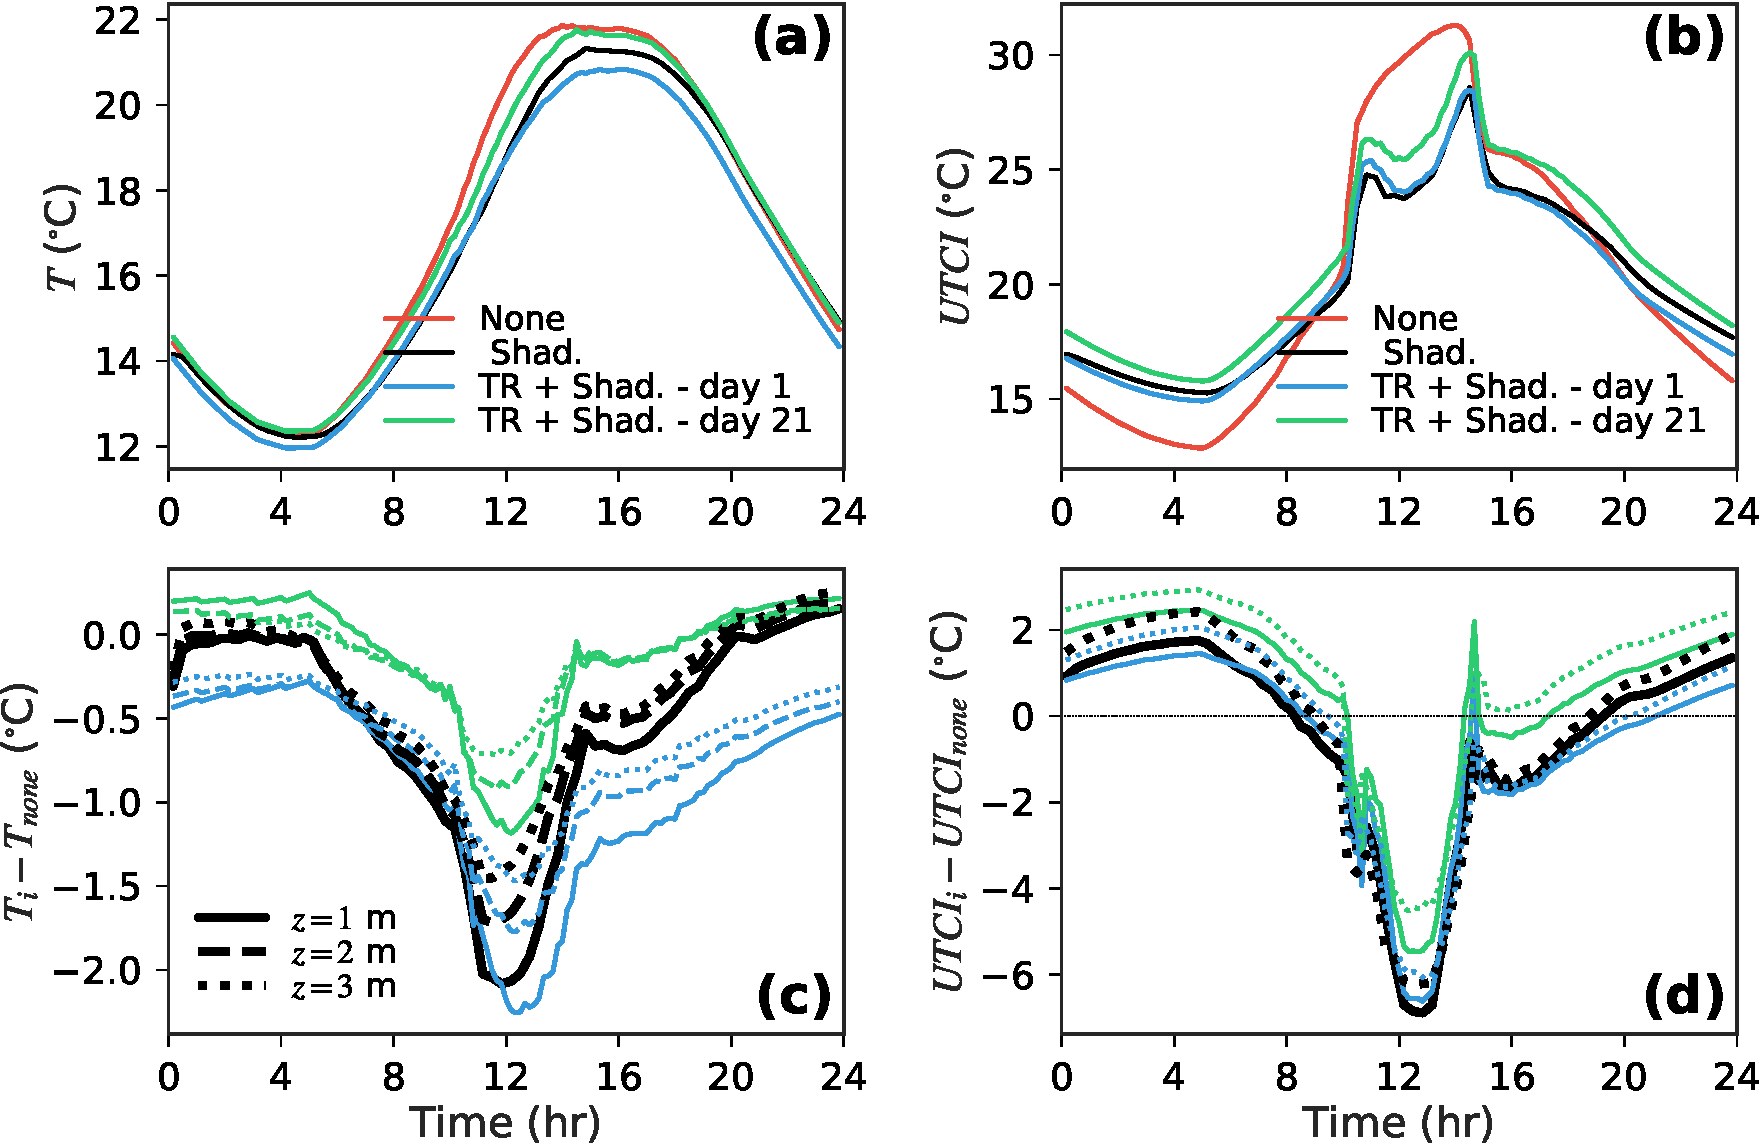
\includegraphics[width=\textwidth]{\figdir/profile_T_UTCI_type3-crop.pdf}
	\caption{Diurnal profile below the vegetation for various cases: no vegetation (\textit{None}), vegetation with only shading at day 1 (\textit{Shad.}), vegetation providing shading and transpirative cooling at day 1 (\textit{TR + Shad. - day 1}), and vegetation providing shading and transpirative cooling at day 1 (\textit{TR + Shad. - day 21}): \subfig{a} air temperature $T$ ($^{\circ}$C) at $(x,y) = (65, 125)$, height $z=2$ m, \subfig{b} universal thermal climate index $\textit{UTCI}$ ($^{\circ}$C) at $(x,y) = (65, 125)$, height $z=2$ m, \subfig{c} Air temperature difference with no vegetation case at $z=[1,2,3]$ m, and \subfig{d} UTCI difference with no vegetation case at $z=[1,3]$ m ($z=2$ removed for brevity).}
	\label{fig:profile_T_UTCI}
\end{figure}

\begin{sidewaysfigure}[p]
	\centering
	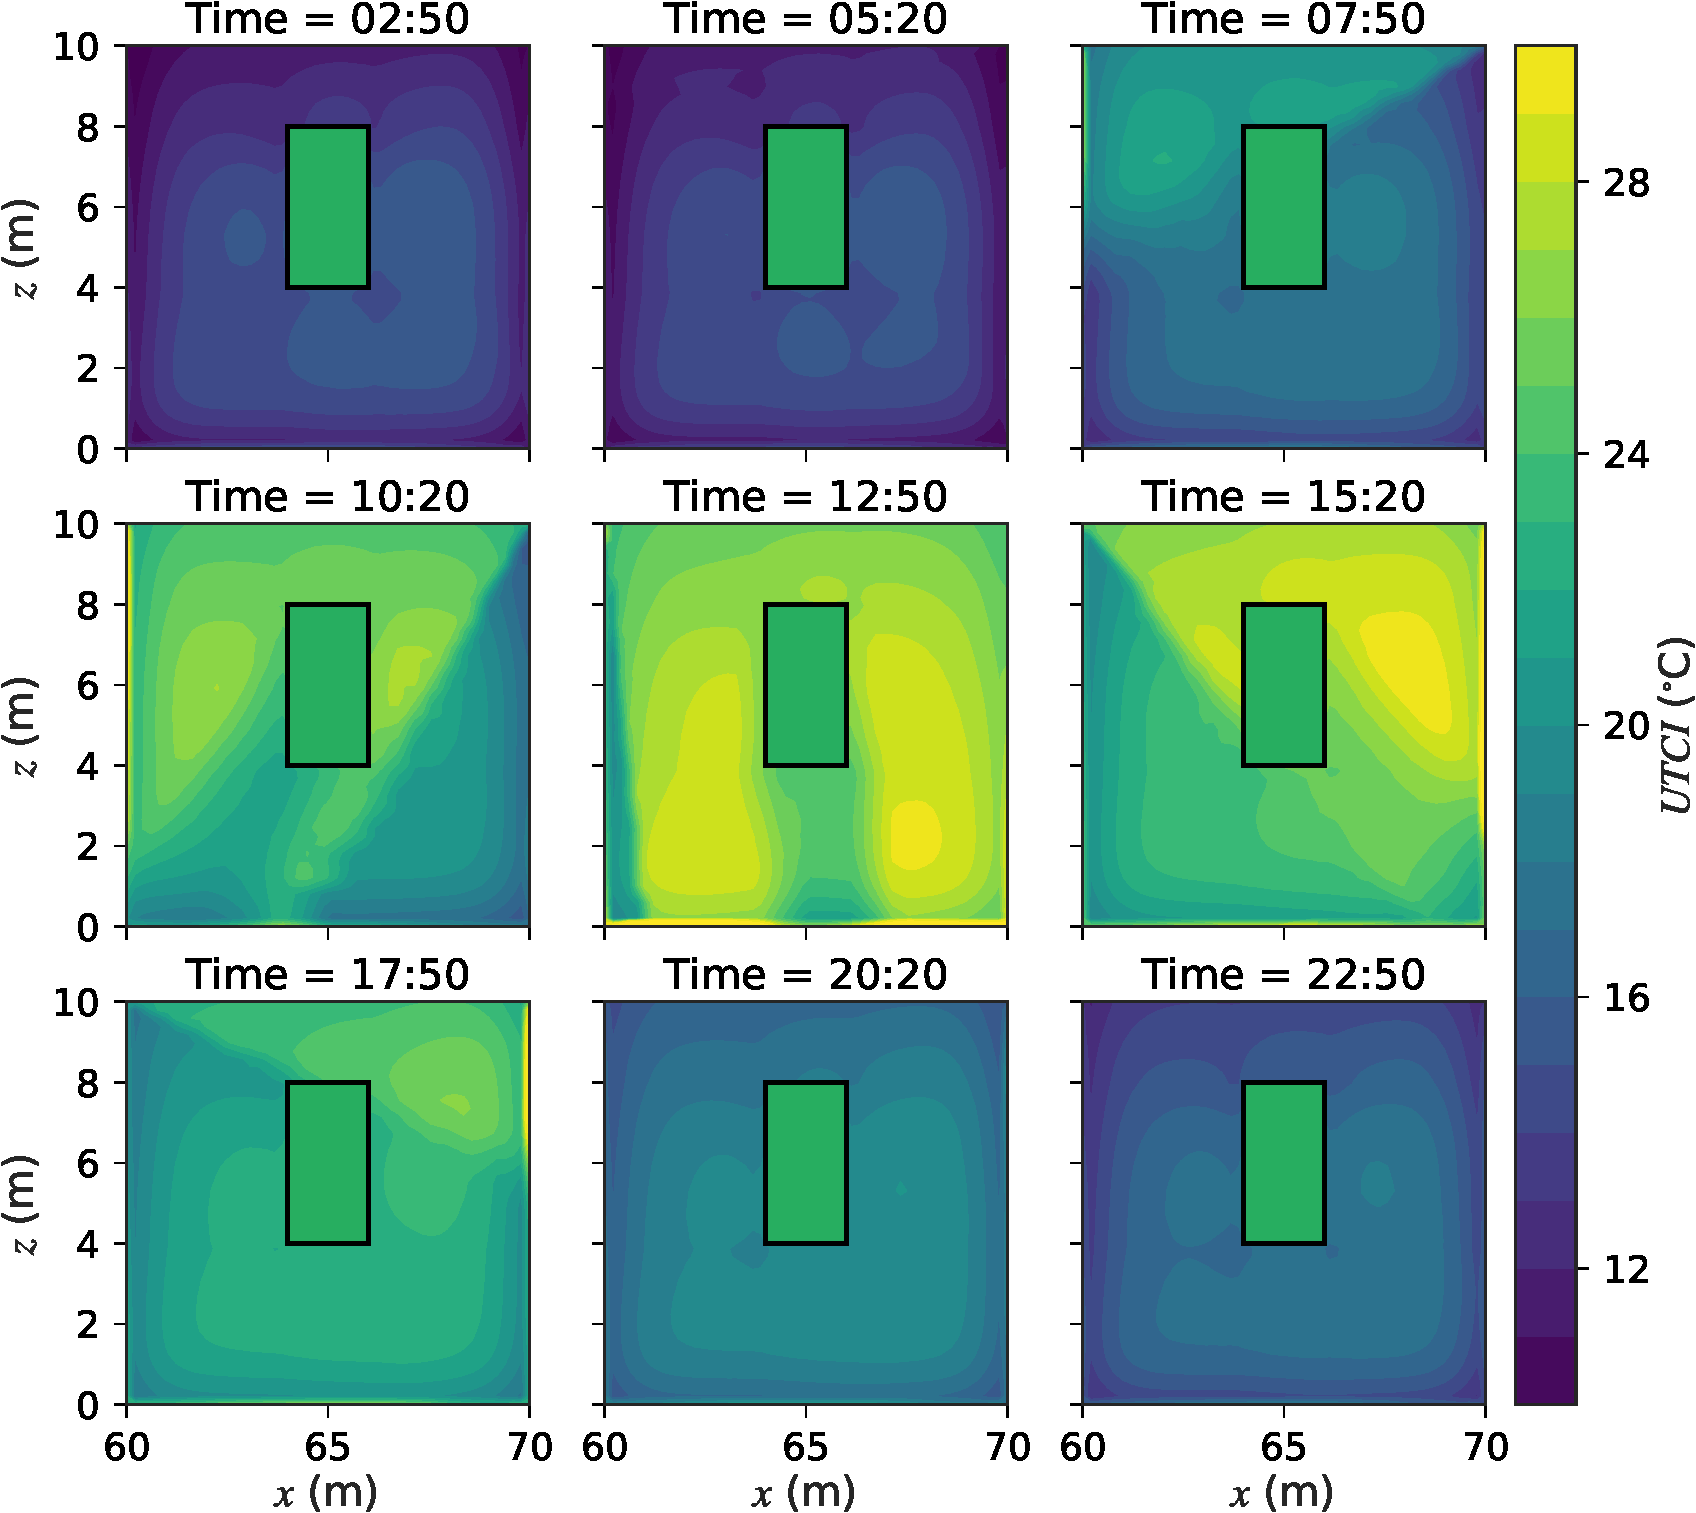
\includegraphics[width=0.8\textwidth]{\figdir/USC_UTCI_type2-crop.pdf}
	\caption{Universal thermal climate index $\textit{UTCI}$ ($^{\circ}$C) inside the street-canyon where the vegetation zone is indicated by a green box. The plot shows the fields with a $150$ minutes interval from $03$:$00$ (HH:MM) to $23$:$00$ (HH:MM).}
	\label{fig:USC_UTCI}
\end{sidewaysfigure}

The influence of vegetation on pedestrian comfort is determined by evaluating the Universal Thermal Climate Index (\textit{UTCI}) ($^{\circ}$C) \citep{Fiala2001,Manickathan2018a}. We employ the formulation used in \cref{ch:parametricstudy}, however, with a more accurate estimation of the mean radiant temperature, as shown in \cref{eq:Tmrt2}, taking in account of the solar altitude change during the day, long-wave and short-wave radiation emitted and reflected from the urban surfaces. \cref{fig:USC_UTCI} shows the $\textit{UTCI}$ ($^{\circ}$C) inside the street-canyon (i.e., $x-z$ plane at $y=125$ m) at 9 separate times of the day. It is apparent that pedestrian comfort is significantly reduced due to the exposure to solar radiation at noon. However, inside the shaded zone of the vegetation, the thermal comfort is substantially improved, as indicated by the reduced UTCI values. In contrast, the impact of humidity generated from vegetation is not discernible in the UTCI distribution. For more clarity, we investigate the diurnal variation of UTCI at a single point and compare with different cases, as seen in \cref{fig:profile_T_UTCI}b. \cref{fig:profile_T_UTCI}b shows that at day, the UTCI is lowest during day 1. When the plant is shading, the thermal comfort improves substantially due to reduced mean radiant temperature. Closer to vegetation, we see that UTCI becomes higher, as shown in \cref{fig:profile_T_UTCI}d, due to the increase in air temperature. By the late afternoon, the UTCI due to additional transpiration is lower than for the case with only shading. However, after 20 days (i.e., day 21), we see a rise in UTCI throughout the day (and night) This is possibly due to transpiration increasing the relative humidity, counterbalancing the cooling provided by the effect of air temperature decrease due to transpiration. The thermal comfort inside the street-canyon is seen to reduce due to the diminished transpiration, higher surface and air temperatures due to radiation trapping. The impact of radiation trapping is especially apparent when comparing the UTCI at night. We see that the lowest UTCI is shown for the case without vegetation. When vegetation is not present, the long-wave radiation is emitted from the surfaces to the sky, thereby cooling the surfaces. However, with extended periods of low water availability, the transpiration benefit provided by vegetation diminishes, and the sustained radiation trapping gradually increases the street-canyon temperature.

% This means the transpiration of the trees does not negatively affect pedestrian comfort in the case studied, although an increase in relative humidity could reduce the thermal comfort.





%Finally, the influence of water availability on thermal comfort is not observable. \textbf{This is because}, the $UTCI$ ($^{\circ}$C) is as shown in \cref{fig:profile_T_UTCI}b. This is because the shading provided by vegetation plays a more important role in thermal comfort. However, an interesting aspect that could be investigated is the influence of water availability on the leaf area density $a$. A wilting of the plant could potentially reduce the shadowing provided by vegetation, which can influence thermal comfort. However, in the present study, this aspect is not investigated.

\subsection{Conclusion}

The present study investigates the influence of transpirative and tree shading on the microclimate of a street canyon. The shading provided by vegetation has a large influence on the street-canyon mean radiant temperature with a drop of around $18$ $^{\circ}$C in the shadow. A significant drop in the mean radiant temperature means a substantial improvement in the measured thermal comfort. At midday, when the solar radiation is at highest, vegetation provides a significant reduction in mean radiation temperature and equally on the thermal comfort. We also observed that, when the plant has sufficient water available, the air temperature below vegetation is also improved due to transpiration. However, with an increasing number of days with reduced water available, the benefits provided by vegetation diminishes over time. This is attributed to reduced plant transpiration due to water stress, lower soil moisture reducing surface evaporation, and the sustained radiation-trapping resulting in larger surface temperatures. Thus, water availability and the nocturnal radiation trapping are important aspects of vegetation when considering them as a mitigation strategy. With an increasing number of days without irrigation, the soil loses the available water for the plant transpiration and for surface evaporative cooling. Furthermore, a prolonged period without irrigation is shown to increase the water stress of the plant (i.e., the difference between leaf and soil water potential), which increases at an exponential rate. Therefore, the demand for irrigation also grows exponentially with time. Urban vegetation irrigation measure should, therefore, take into account the growth in water stress when exposed to a prolonged period of drought. Such conditions can be more frequent in today's changing climate. Furthermore, the nocturnal radiation trapping shows that, vegetation, counter-intuitively stagnates the cooling of cities during the night. So, cities should not ignore this contribution of vegetation when employing UHI mitigation measures using vegetation. Finally, we observed that the complex modeling approach implemented in this study can capture import plant dynamics such as hydraulic redistribution. It can have an important contribution to the water availability of the shallow-rooted plant species such as grass or small shrubs.

% The study shows that transpiration has a direct influence in the plant vicinity air temperature and negligible effects on the thermal comfort measured through the Universal Thermal Climate Index (UTCI). 

%In contrast, the shading provided by vegetation has a large influence on the street-canyon mean radiant temperature with a drop of around $18$ ($^{\circ}$C) in the shadow. A significant drop in the mean radiant temperature means a substantial improvement in the measured thermal comfort. An important aspect of vegetation that should be taken into account is the nocturnal radiation trapping due to the presence of vegetation. At night, due to obstruction of long-wave radiation emission from urban surfaces to the sky, the mean radiant temperature and similarly the UTCI is higher during night time. 

%Another aspect that also plays an important role is water availability. With an increasing number of days without irrigation, the soil loses the available water for the plant transpiration. 

%We observed that due to this, the transpiration rate decays, resulting in an increase in the sensible heat flux from vegetation. 

 


\section{Case study: Muensterhof}

The Muensterhof case study demonstrates the application of the developed model to a realistic urban setting. The Muensterhof is a town square within the city of Zurich that currently lacks vegetation. In this study, we investigate the influence of vegetation and the impact on the atmospheric conditions such as air temperature, relative humidity and furthermore, the contribution of foliage to intercepting the short-wave radiation. 

\subsection{Simulation setup}
\label{sec:muenstersetup}

\begin{figure}[t]
	\centering
	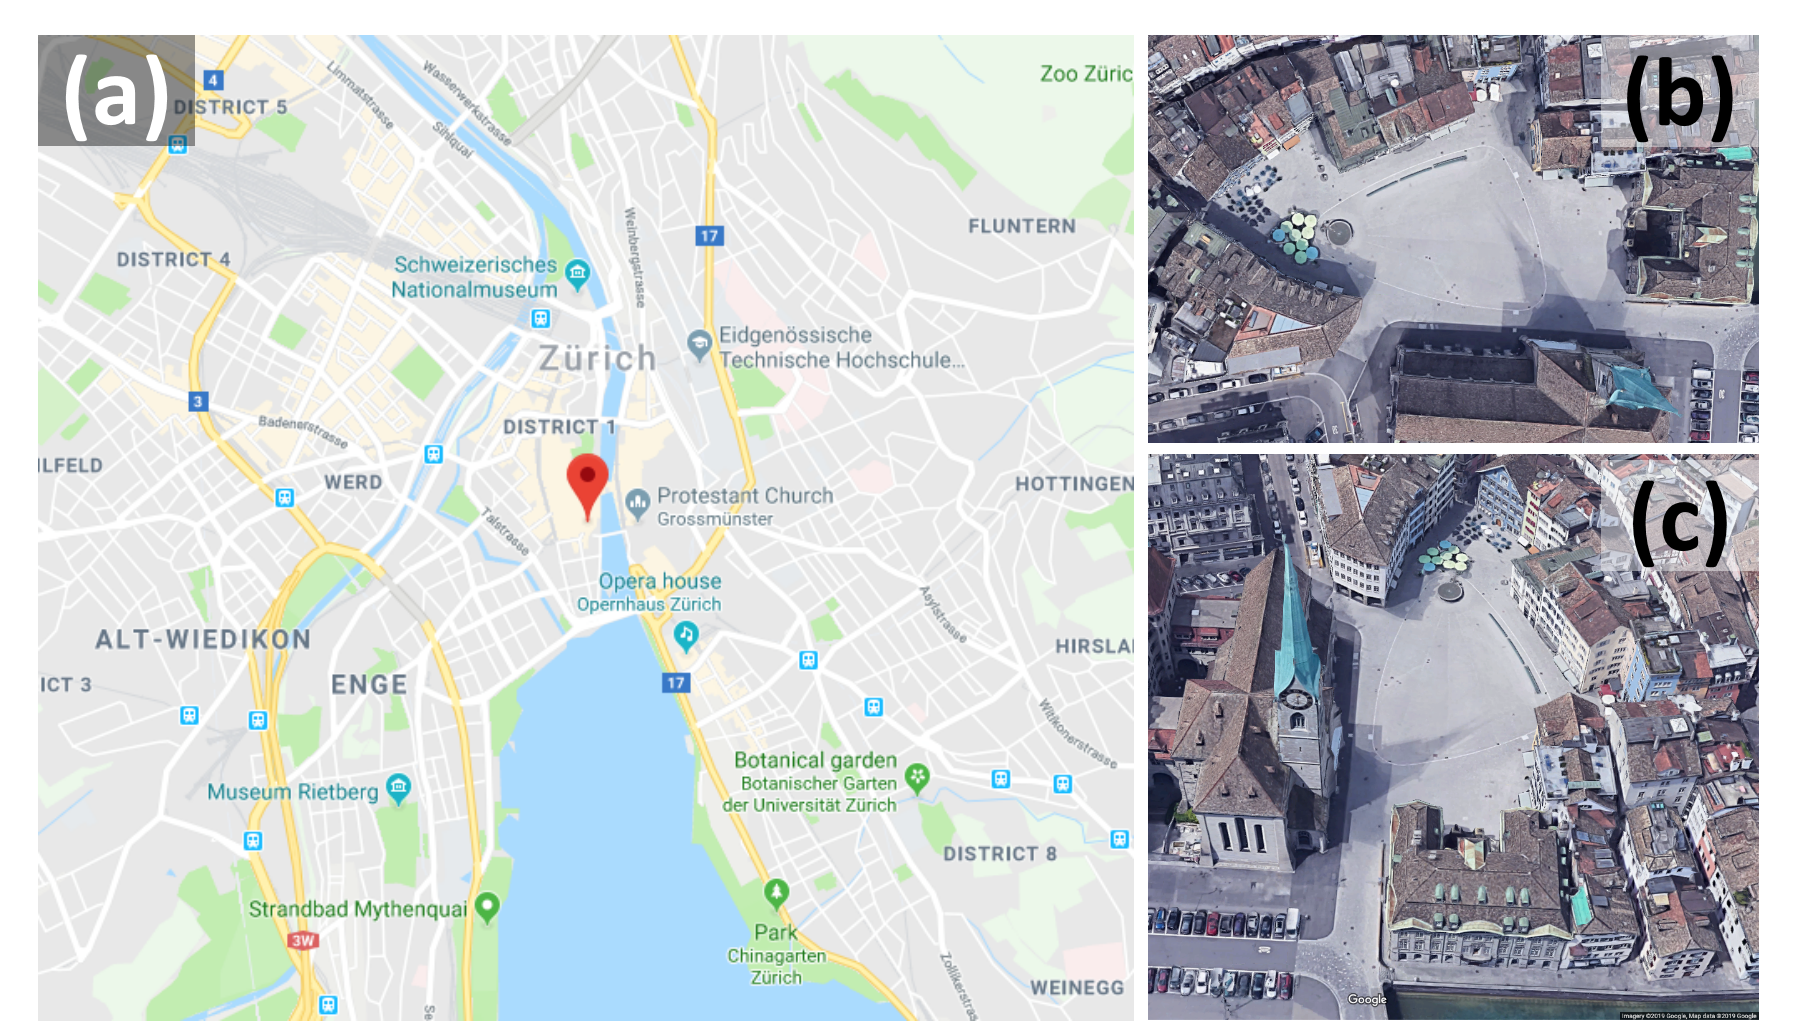
\includegraphics[width=\textwidth]{\figdir/muensterhof_view_type2.png}
	\caption{Satellite view of the Muensterhof obtained from Google Map Data showing: \subfig{a} map view, \subfig{b} top view (i.e., eagle eyes view), and \subfig{c} west-looking view of the Muensterhof square.}
	\label{fig:muensterhof_view}
\end{figure}

The simulation is performed focusing on the Muensterhof square (see \cref{fig:muensterhof_view}). Therefore, highest level of building details is found near the square and to increase the computation performance, the level of detail is reduced further away from the square. Similarly, the mesh is refined with highest level of refinement inside the Muensterhof square. \cref{fig:mesh_resolution_muensterhof_tree} shows the surface layer close to the building walls with i) a single isolated tree inside the square, and ii) multiple tree configuration with 4 identical trees. In the first case, the numerical domain is discretized into $\num{4432297}$ cells with minimum cell size of $\num{2.38e-3}$ m$^{3}$ near the building and similarly, $\num{4453514}$ cells in the second case with multiple trees.

%\begin{sidewaysfigure}[p]
%	\centering
%	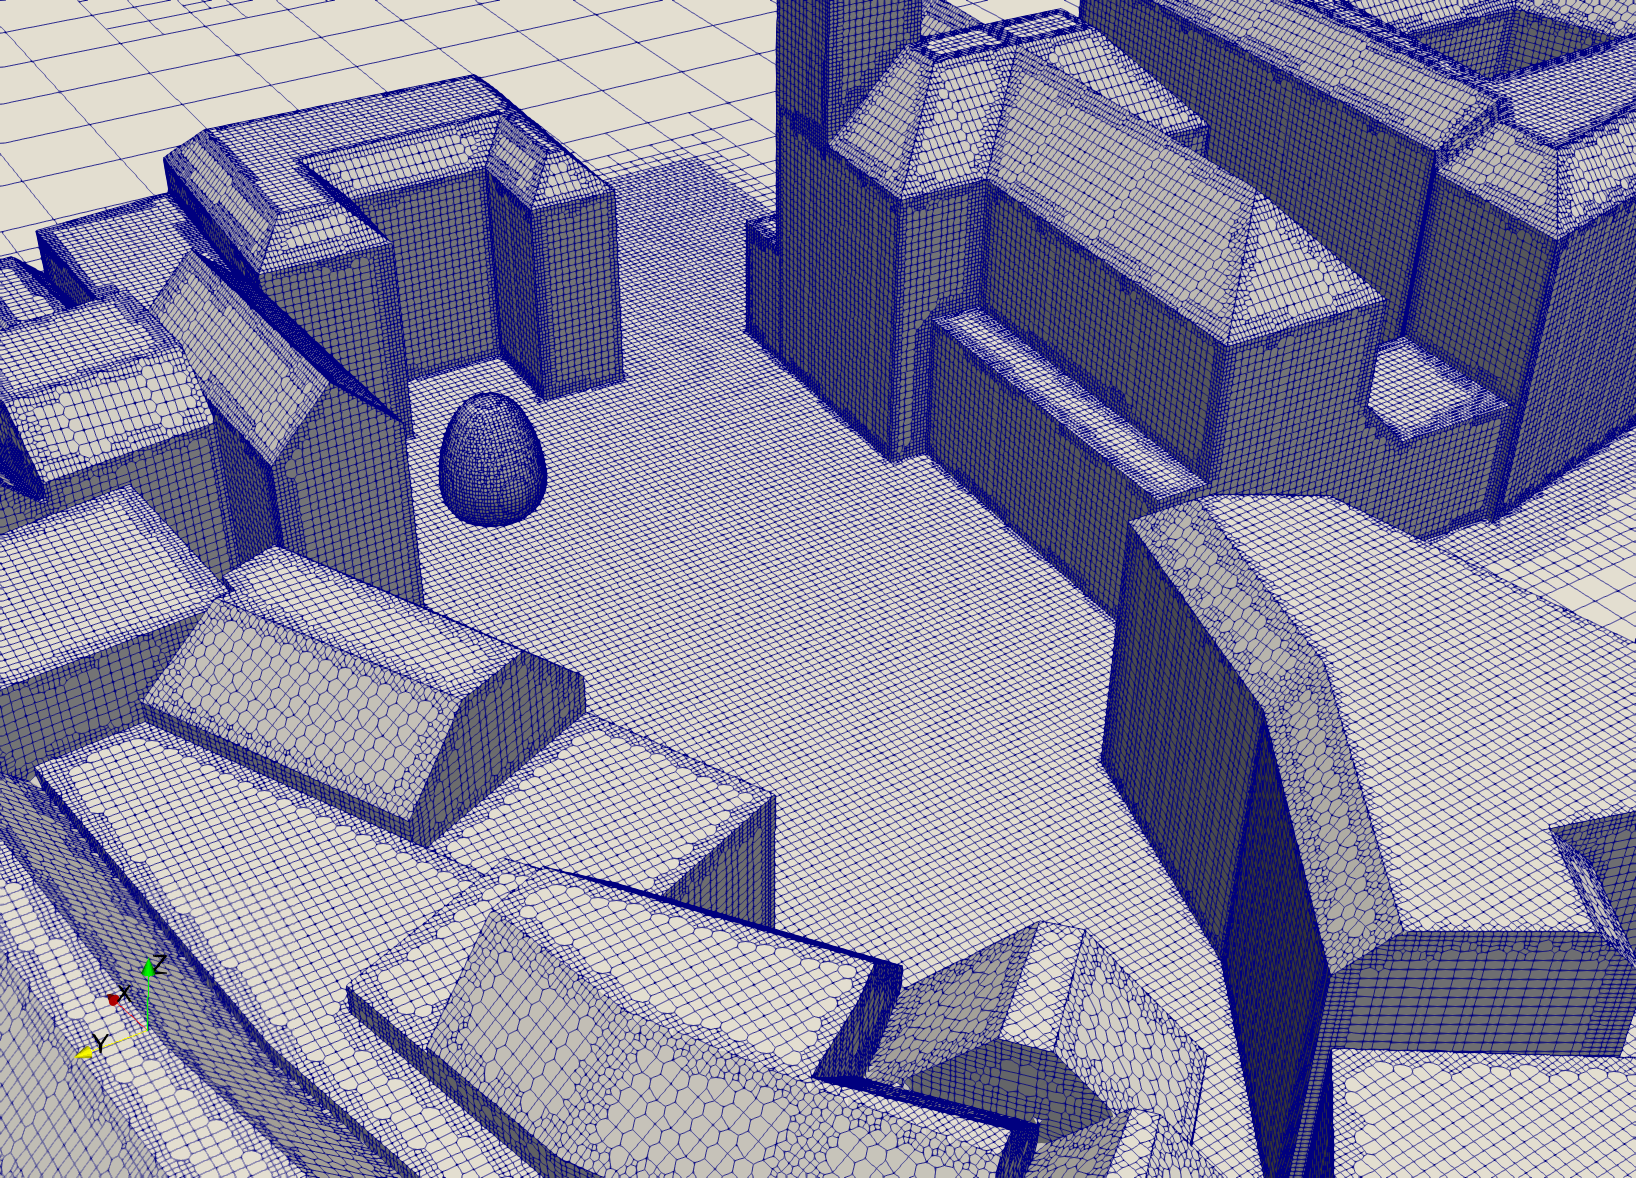
\includegraphics[width=0.8\textwidth]{\figdir/mesh_resolution_muensterhof_tree_V2.png}
%	\caption{Simulation sub-domain showing the surface layer mesh refined closed to the building walls in Muensterhof along with a single isolated tree. The numerical domain is discretized into $\num{4432297}$ cells with minimum cell size of $\num{2.38e-3}$ m$^{3}$ near the building.}
%	\label{fig:mesh_resolution_muensterhof_tree}
%\end{sidewaysfigure}
%mesh_resolution_muensterhof_treegroupA_V2
%\begin{figure}[p]
%	\centering
%	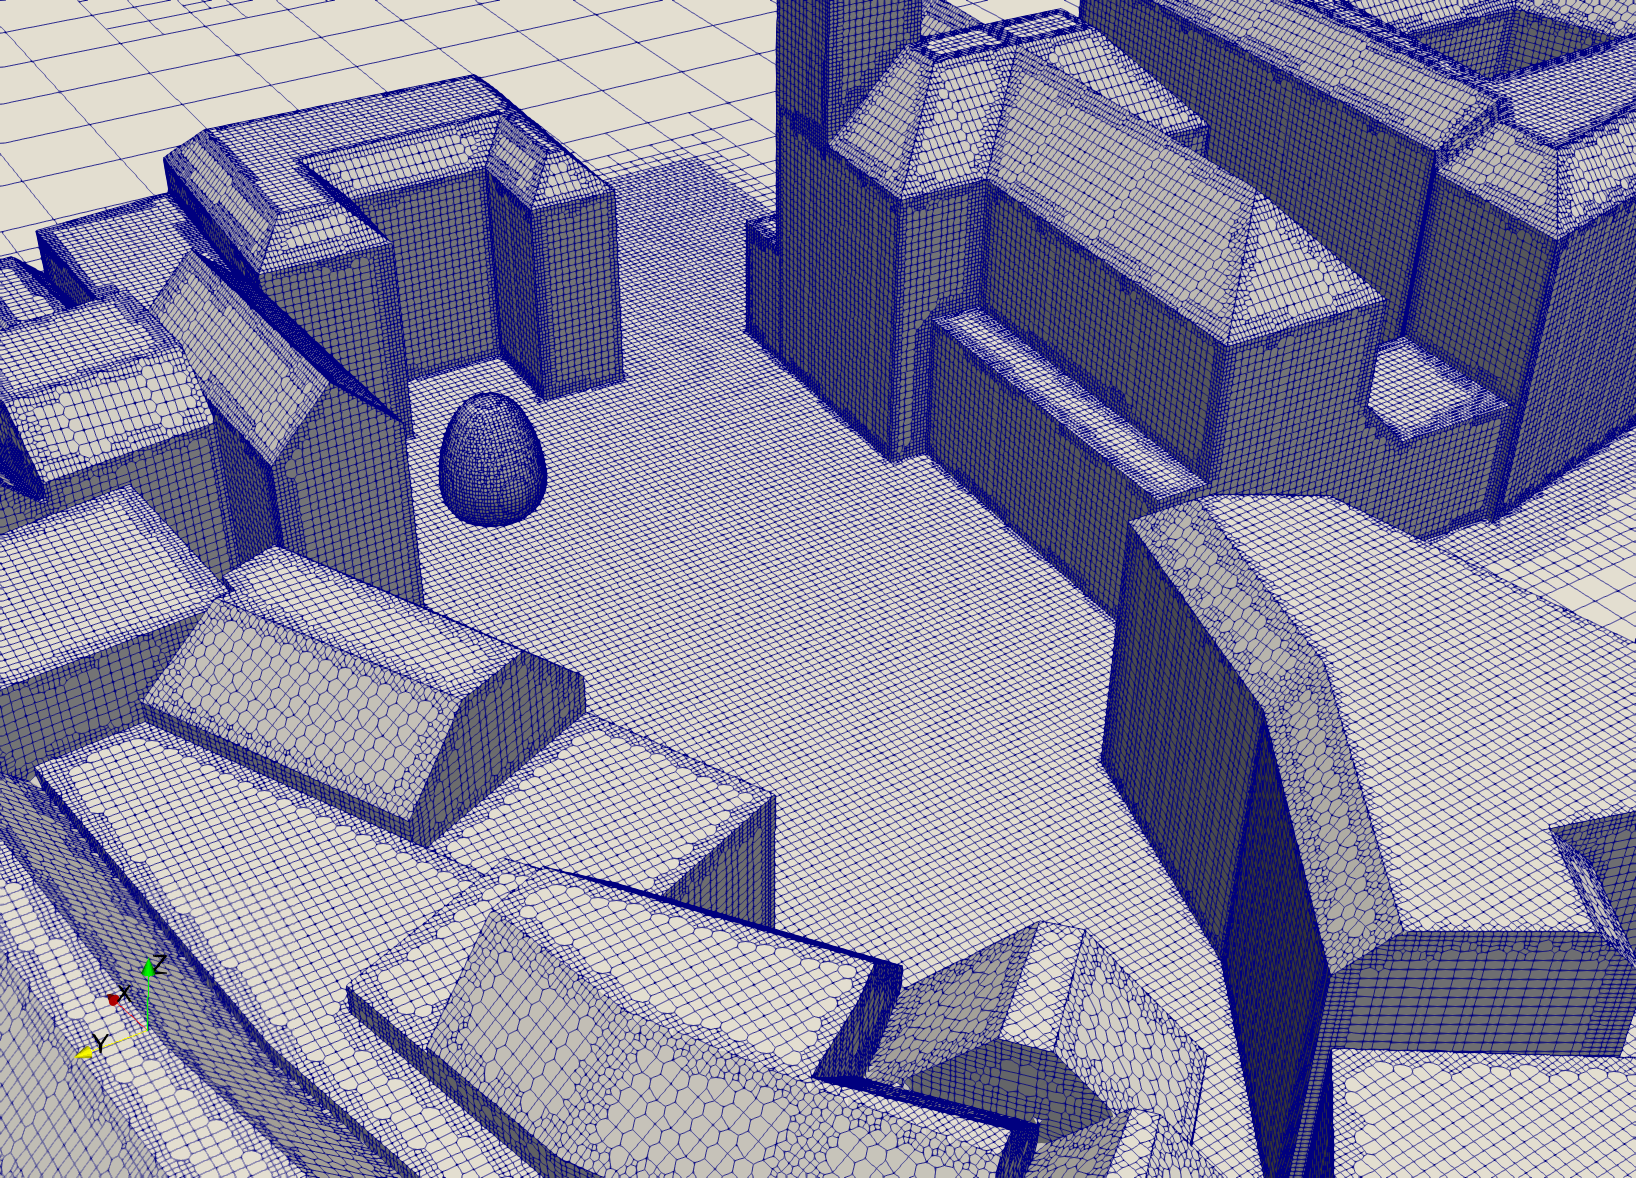
\includegraphics[width=0.8\textwidth]{\figdir/mesh_resolution_muensterhof_tree_V2.png}
%	\caption{Simulation sub-domain showing the surface layer mesh refined closed to the building walls in Muensterhof along with a single isolated tree. The numerical domain is discretized into $\num{4432297}$ cells with minimum cell size of $\num{2.38e-3}$ m$^{3}$ near the building.}
%	\label{fig:mesh_resolution_muensterhof_tree}
%\end{figure}

\begin{figure}[p]
	\centering
%	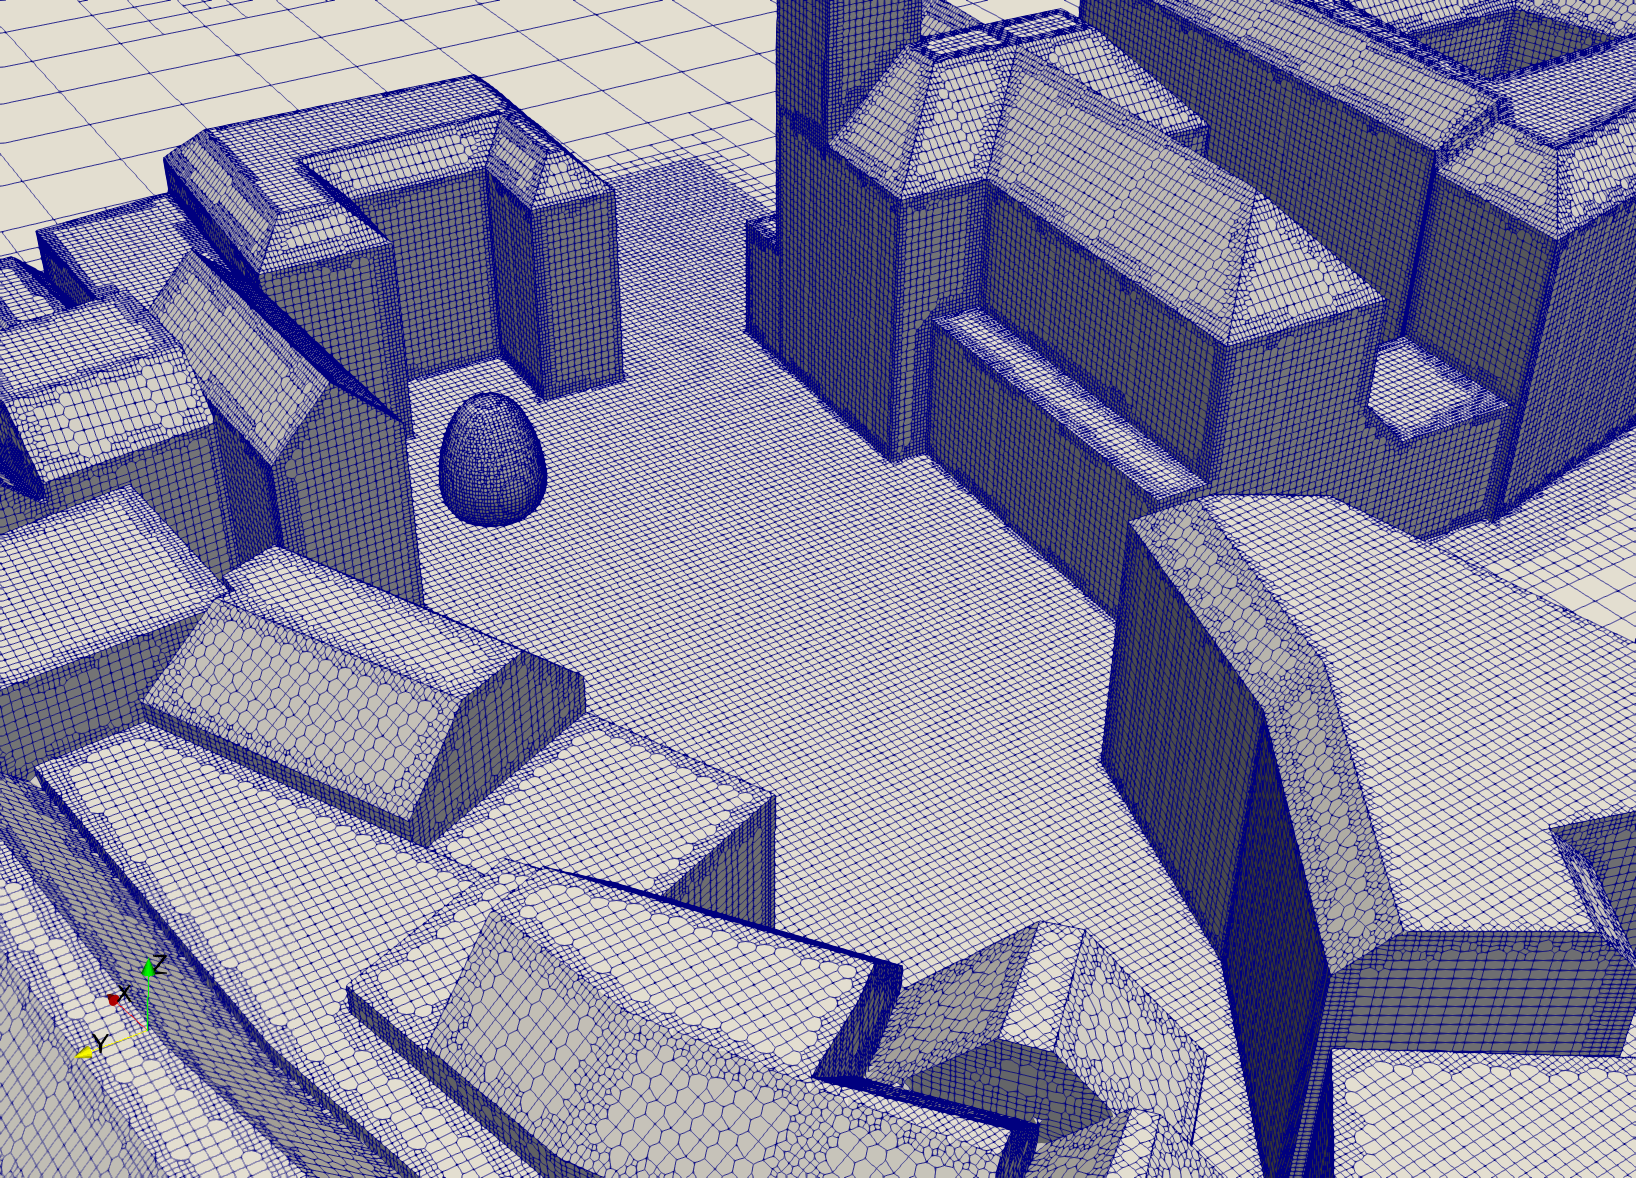
\includegraphics[width=0.8\textwidth]{\figdir/mesh_resolution_muensterhof_tree_V2.png}
%	\caption{Simulation sub-domain showing the surface layer mesh refined closed to the building walls in Muensterhof along with a single isolated tree. The numerical domain is discretized into $\num{4432297}$ cells with minimum cell size of $\num{2.38e-3}$ m$^{3}$ near the building.}
	\begin{subfigure}[b]{0.8\linewidth}
		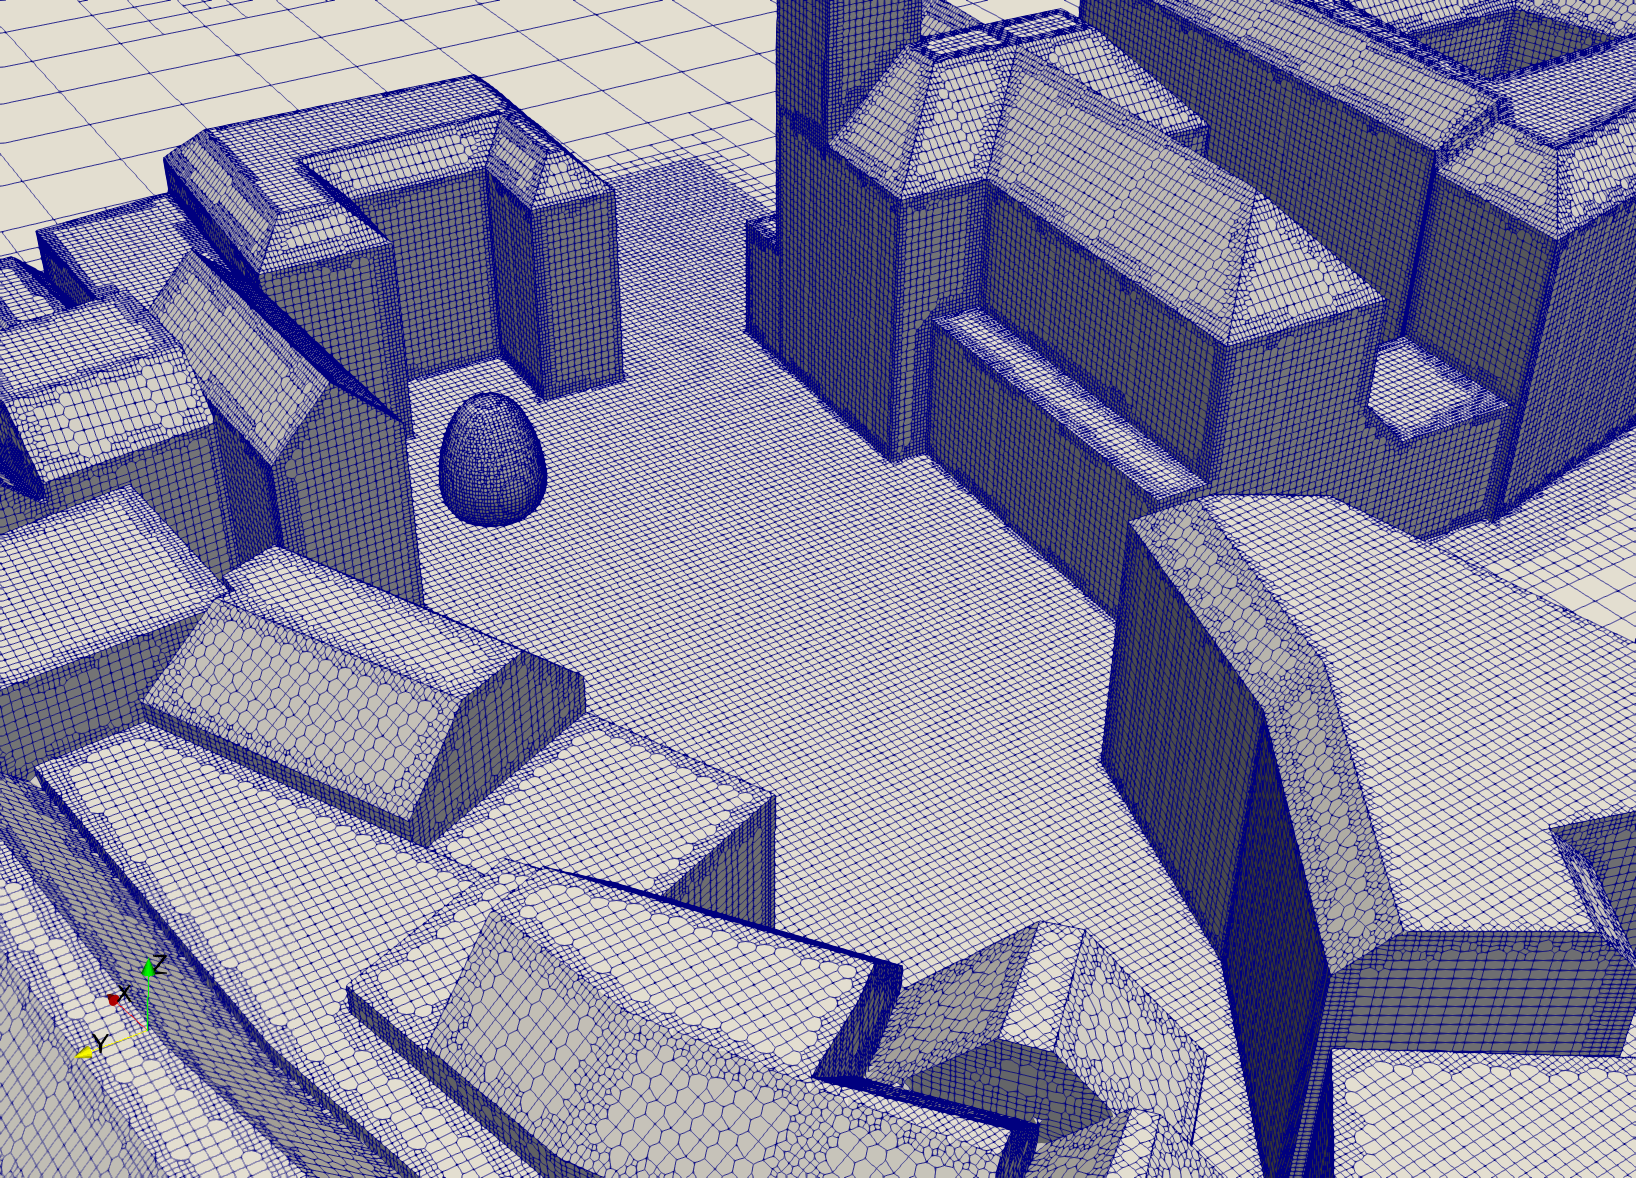
\includegraphics[width=\linewidth]{\figdir/mesh_resolution_muensterhof_tree_V2.png}
		\caption{A single isolated tree: $N_{\textit{cells}} = \num{4432297}$}%\label{fig:w_basecase_1200}
	\end{subfigure}
	
	\medskip
	
	\begin{subfigure}[b]{0.8\linewidth}
		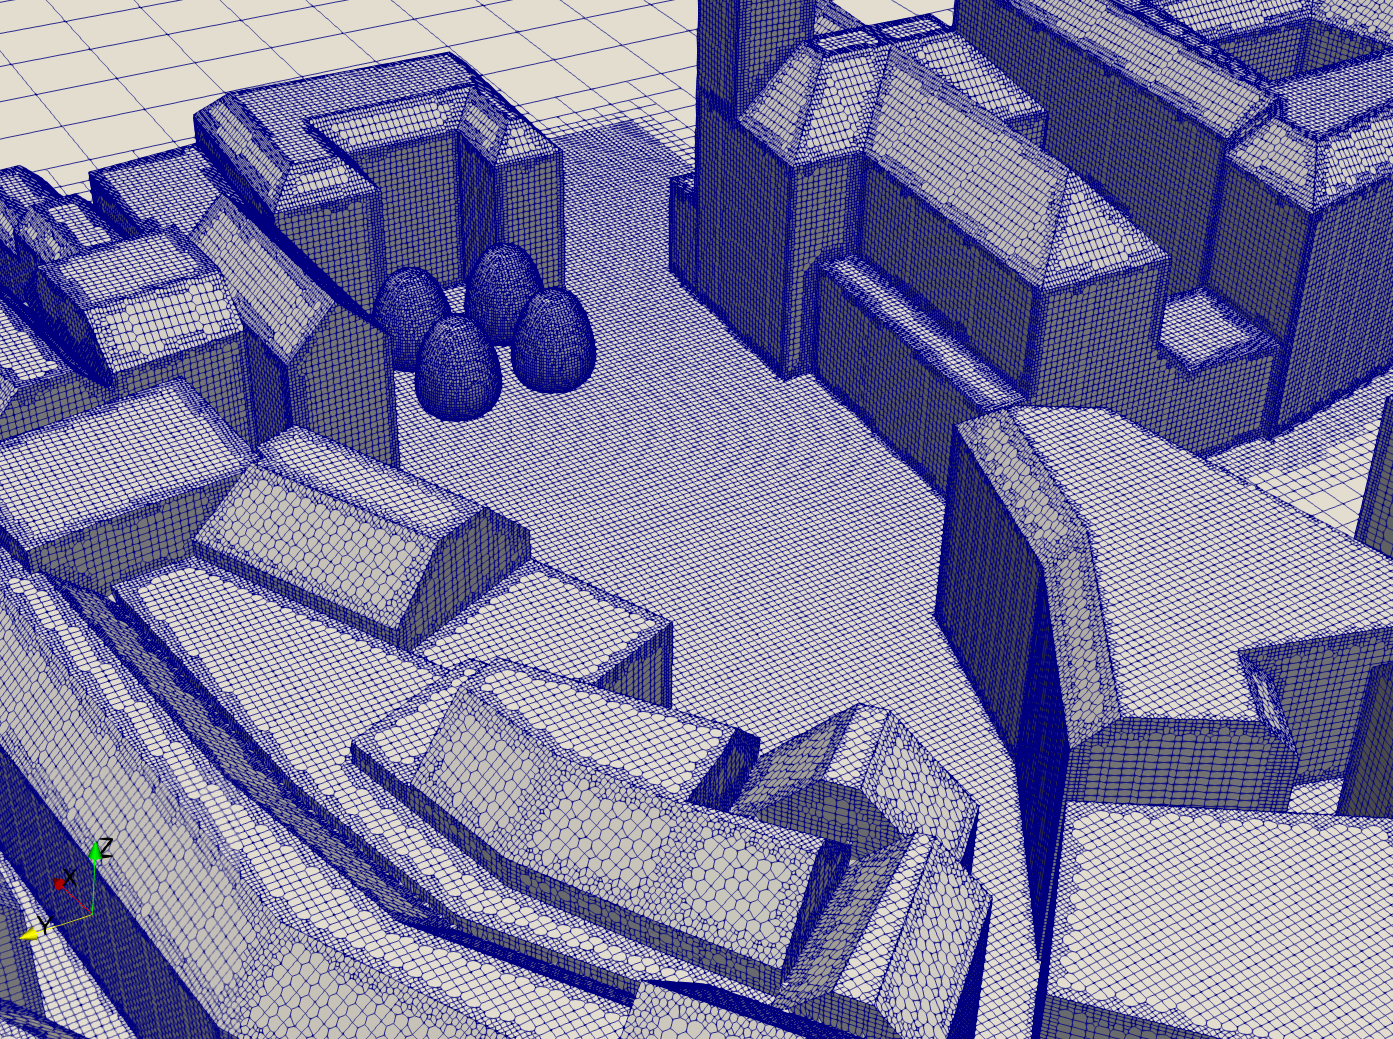
\includegraphics[width=\linewidth]{\figdir/mesh_resolution_muensterhof_treegroupA_V2.png}
		\caption{A group of four trees: $N_{\textit{cells}} = \num{4453514}$}%\label{fig:w_tree_1200}
	\end{subfigure}
	\caption{Simulation sub-domain showing the surface layer mesh refined closed to the building walls in Muensterhof.}
	\label{fig:mesh_resolution_muensterhof_tree}
\end{figure}

\begin{figure}[p]
	\centering
	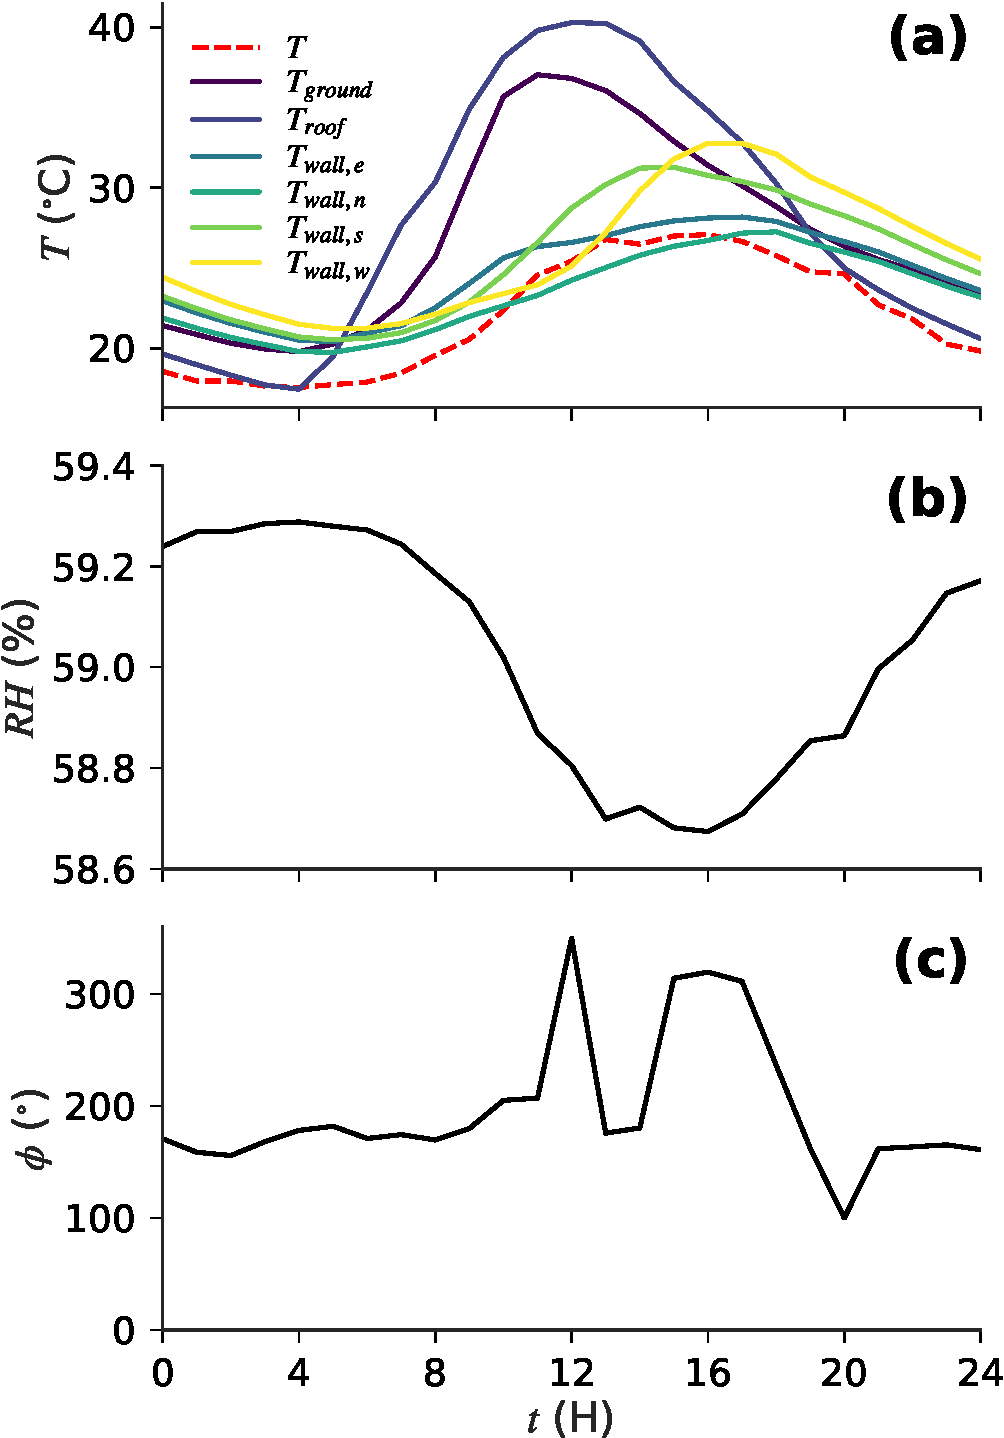
\includegraphics[width=0.7\textwidth]{\figdir/muensterhof_basecase_bc-crop.pdf}
	\caption{Boundary conditions obtained from mesoscale model: \subfig{a} air temperature $T$ ($^{\circ}$C), ground temperature $T_{\textit{ground}}$ ($^{\circ}$C) (note: only for the ground outside the Muensterhof square), roof temperature $T_{\textit{roof}}$ ($^{\circ}$C), wall temperatures $T_{\textit{wall}}$ ($^{\circ}$C) for north (N), south (S), east (E), and west side (W); \subfig{b} relative humidity $RH$ (\%); \subfig{c} wind direction $\phi$ ($^{\circ}$). }
	\label{fig:muensterhof_bc}
\end{figure}


The location of the trees are chosen based on the requirements of the city of Zurich. The eastern exit towards the river Limmat is required to be unrestricted to enable transport to and from Muensterhof square. Furthermore, the center of the Muensterhof is required to be unrestricted to provide space of public events. A possible region that can be utilized for trees is near the north-east corner of the square, as indicated in \cref{fig:mesh_resolution_muensterhof_tree}. Therefore, trees was placed at this location to study the influence of vegetation. The tree has a radius of $4$ m and a high of $10$ m with foliage base at $2$ m. The simulation is driven with boundary conditions obtained from mesoscale simulation of Zurich, see \cref{fig:muensterhof_bc}. The solar radiation intensity and the wall function are applied as described in the previous sections. Similarly, the plant properties are set to similar that of the previous study of vegetation in the urban street canyon. 

\subsection{Results and Discussion}

\subsubsection{Single tree case}

\begin{figure}[p]
	\centering
	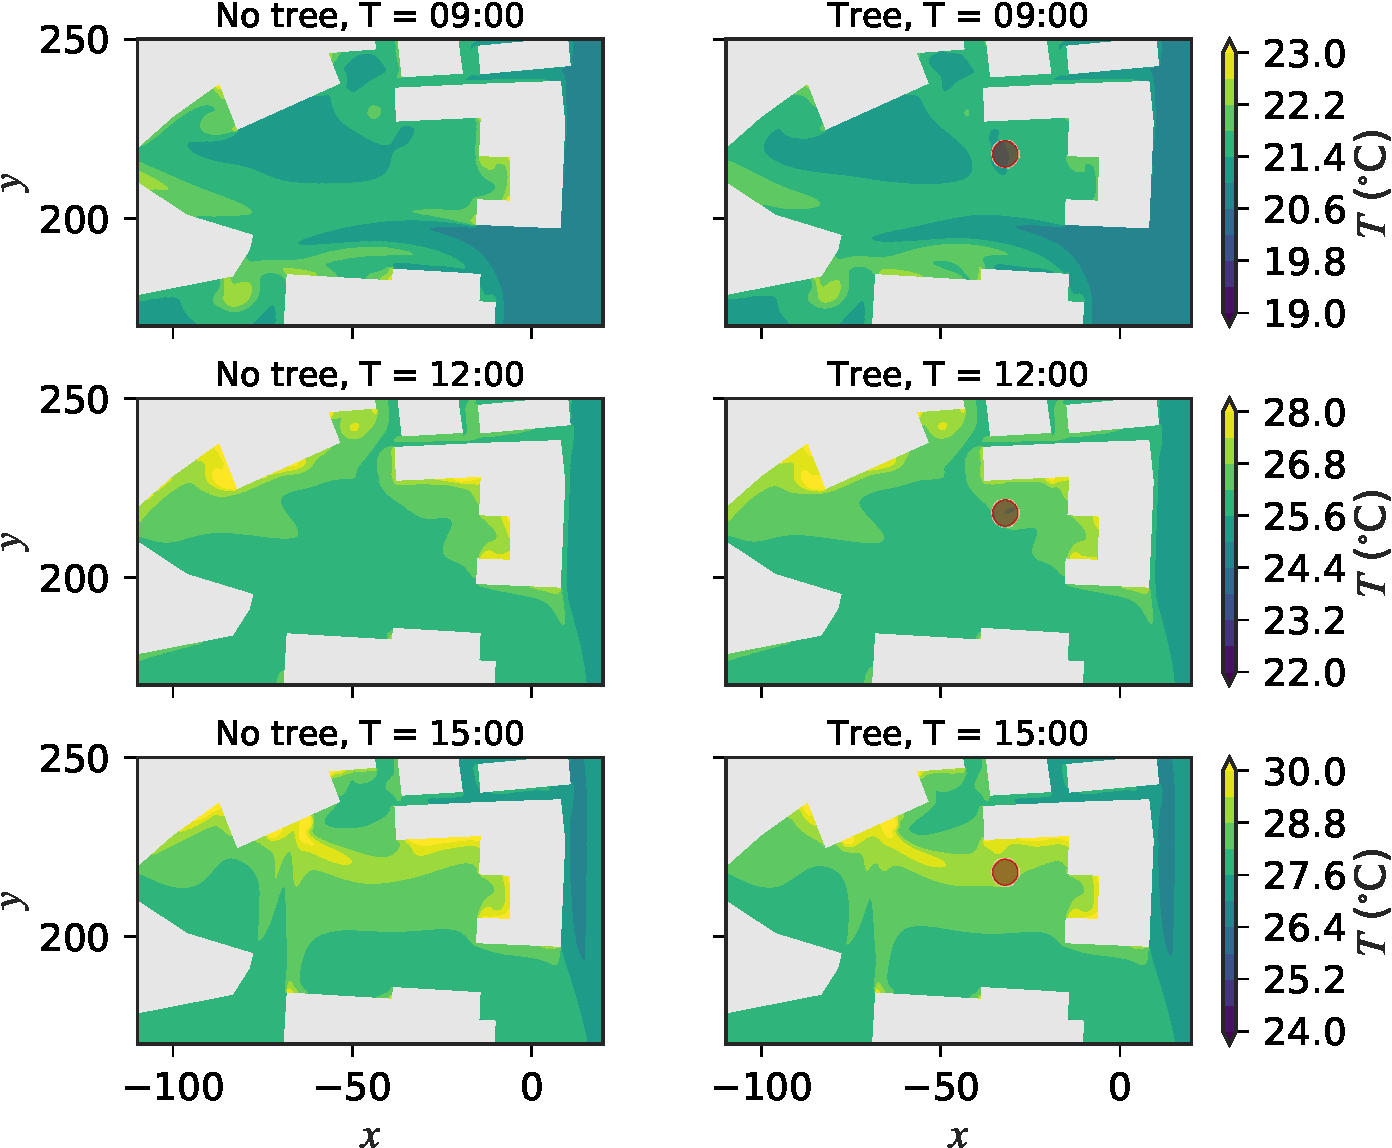
\includegraphics[width=\textwidth]{\figdir/mhof_tree_and_notree_T_type2-crop.pdf}
	\caption{Air temperature $T$ ($^{\circ}$C) at $z=4$ m at 3 different times of the day (09:00, 12:00, and 15:00 (HH:MM)). The region of tree is indicated by a red outline.}
	\label{fig:T_muensterhof}
\end{figure}

\begin{figure}[p]
	\centering
	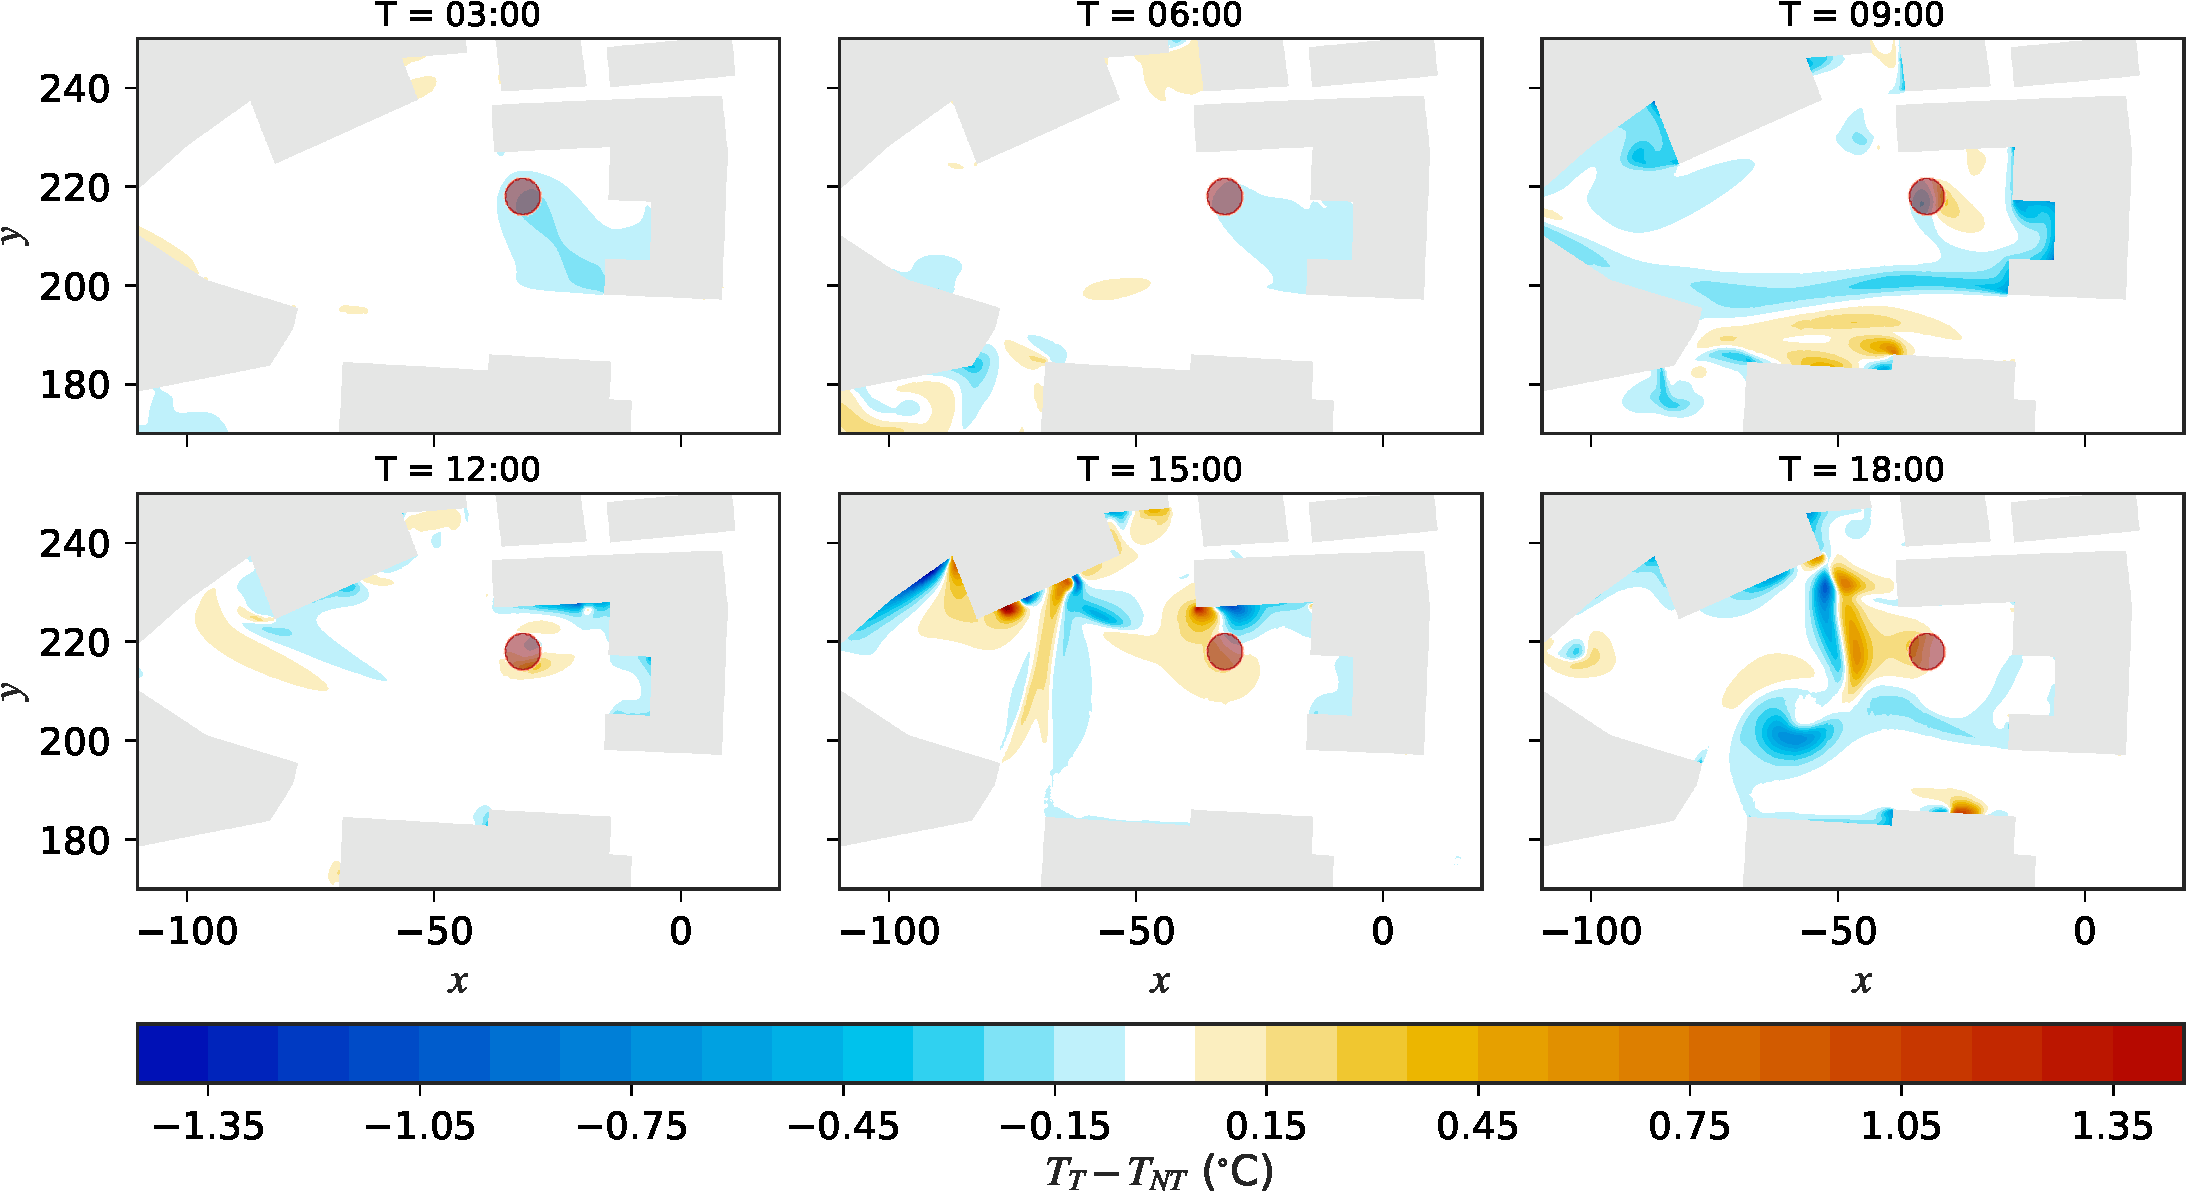
\includegraphics[width=\textwidth]{\figdir/mhof_tree_vs_notree_T_type2-crop.pdf}
	\caption{Air temperature difference $T_{T}-T_{\textit{NT}}$ ($^{\circ}$C) between the cases \textit{with} (T) and \textit{without} (NT) tree at $z=4$ m at 6 different times of the day (03:00, 06:00, 09:00, 12:00, 15:00, and 18:00 (HH:MM)).}
	\label{fig:Tdiff_muensterhof}
\end{figure}

\begin{figure}[p]
	\centering
	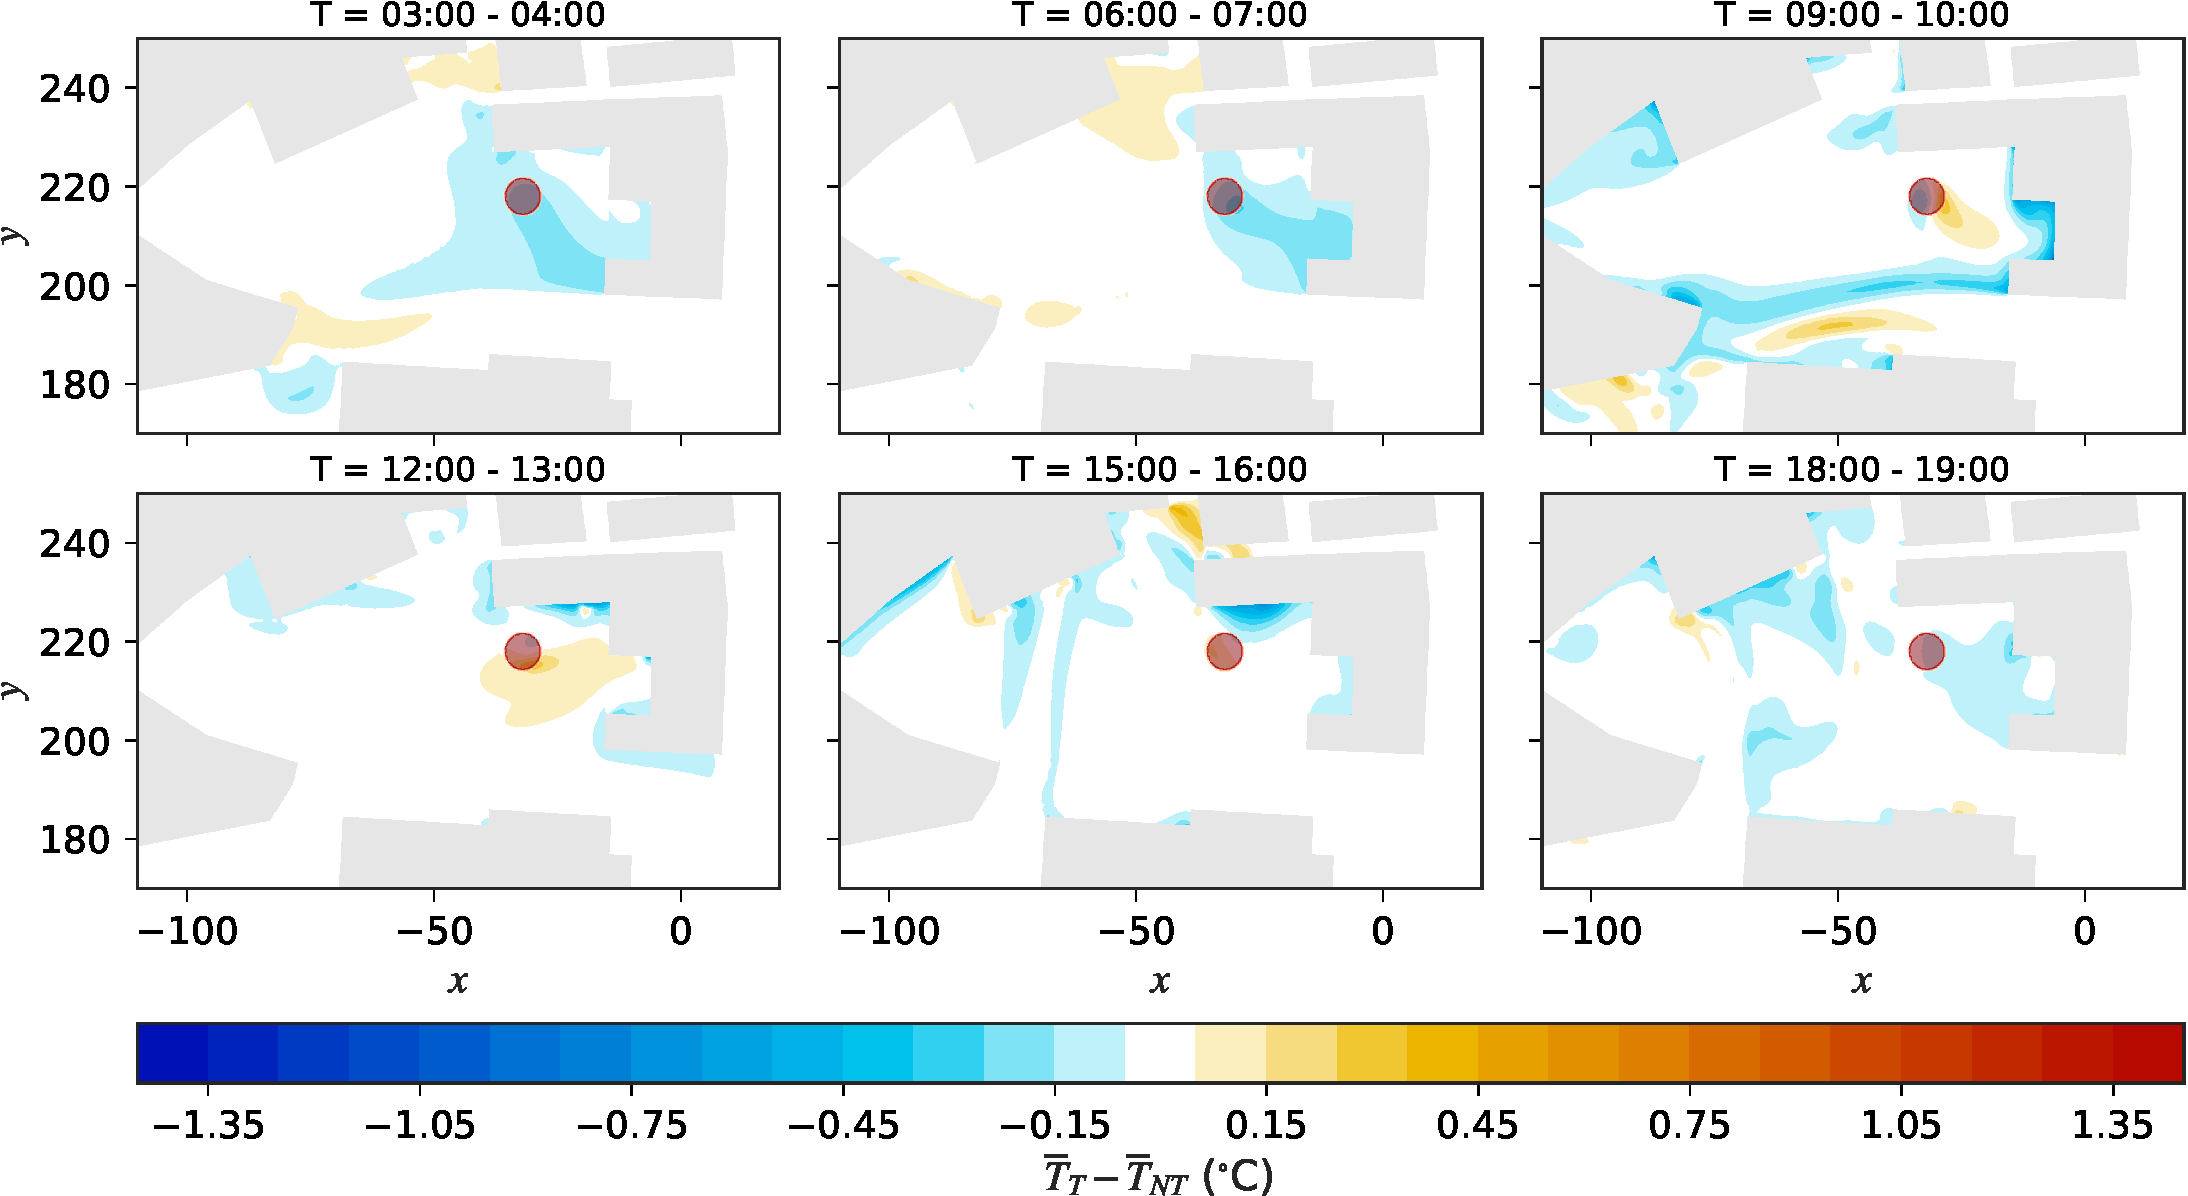
\includegraphics[width=\textwidth]{\figdir/mhof_tree_vs_notree_T_hourlyaveraged_type2-crop.pdf}
	\caption{Hourly-averaged $\overline{T}_{T}-\overline{T}_{\textit{NT}}$ ($^{\circ}$C) at $z=4$ m between 6 different times of the day (03:00 - 04:00, 06:00 - 07:00, 09:00 - 10:00, 12:00 - 13:00, 15:00 - 16:00, and 18:00 - 19:00).}
	\label{fig:Tdiff_muensterhof_hourly}
\end{figure}

The single tree case simulation is ran for two different configuration: \textit{with} and \textit{without} tree. \cref{fig:T_muensterhof} shows the air temperature $T$ ($^{\circ}$C) at $z=4$ m (i.e., $x-y$ plane) at 3 different time of the day (09:00, 12:00, and 15:00 (HH:MM)). The tree is outlined using a red outline to indicate its location. We observe that there is only a slight change in the air temperature contours. However, as it is hard to discern, \cref{fig:Tdiff_muensterhof} shows the air temperature difference between the \textit{with} and \textit{without} tree case. We also investigate additional times of the day (03:00, 06:00, 09:00, 12:00, 15:00, and 18:00). We see that the strongest change in air temperature occurs during day time, mainly when shading and plant transpiration occurs. Furthermore, the influence of a single tree is observed to affect the entire square and the strongest change in air temperature occurring at walls near the tree. However, we also observe that near the north-west region of the square, a hot spot is present near the wall. The cause of this is not obvious and could be due to changes in the flow field shifting the hot-spot as we also observe a cold-spot directly nearby. To take into account of possible time-shift effects, the air temperature difference is performed for the hourly-averaged values. \Cref{fig:Tdiff_muensterhof_hourly} shows the hourly-averaged air temperature difference between the cases \textit{with} and \textit{without} tree between 6 different times of the day (03:00 - 04:00, 06:00 - 07:00, 09:00 - 10:00, 12:00 - 13:00, 15:00 - 16:00, and 18:00 - 19:00 (HH:MM)). Comparing the hourly-averaged with the 10-minute averaged plot (i.e., \Cref{fig:Tdiff_muensterhof}), we notice the strong difference in the air temperatures has diminished. This indicates that the high temperature difference was predominately due to a time-shift in the temperature profile. Studying the hourly-averaged temperature field, we see that a single tree generally provides cooling to the flow. Between 15:00 and 16:00, we observe that the building walls close to the tree are cooler with up to $1$ $^{\circ}$C drop in air temperature. During night-time, we see that the changes in the air temperature due to vegetation reduces. \cref{fig:wdiff_muensterhof} shows the humidity ratio difference between the cases \textit{with} (T) and \textit{without} (NT) tree $\overline{w}_{T}-\overline{w}_{\textit{NT}}$ (g\,kg$^{-1}$). We see that vegetation is an important source of humidity in the Muensterhof as high values of humidity ratio is convected from the foliage especially during afternoon when solar radiation is present. Due to the wind direction, the humidity is most convected towards the building on the north-east side. It could potential have an influence on the moisture content of the building walls and thereby influencing cooling from evaporative drying of the surfaces. 

\begin{figure}[t]
	\centering
	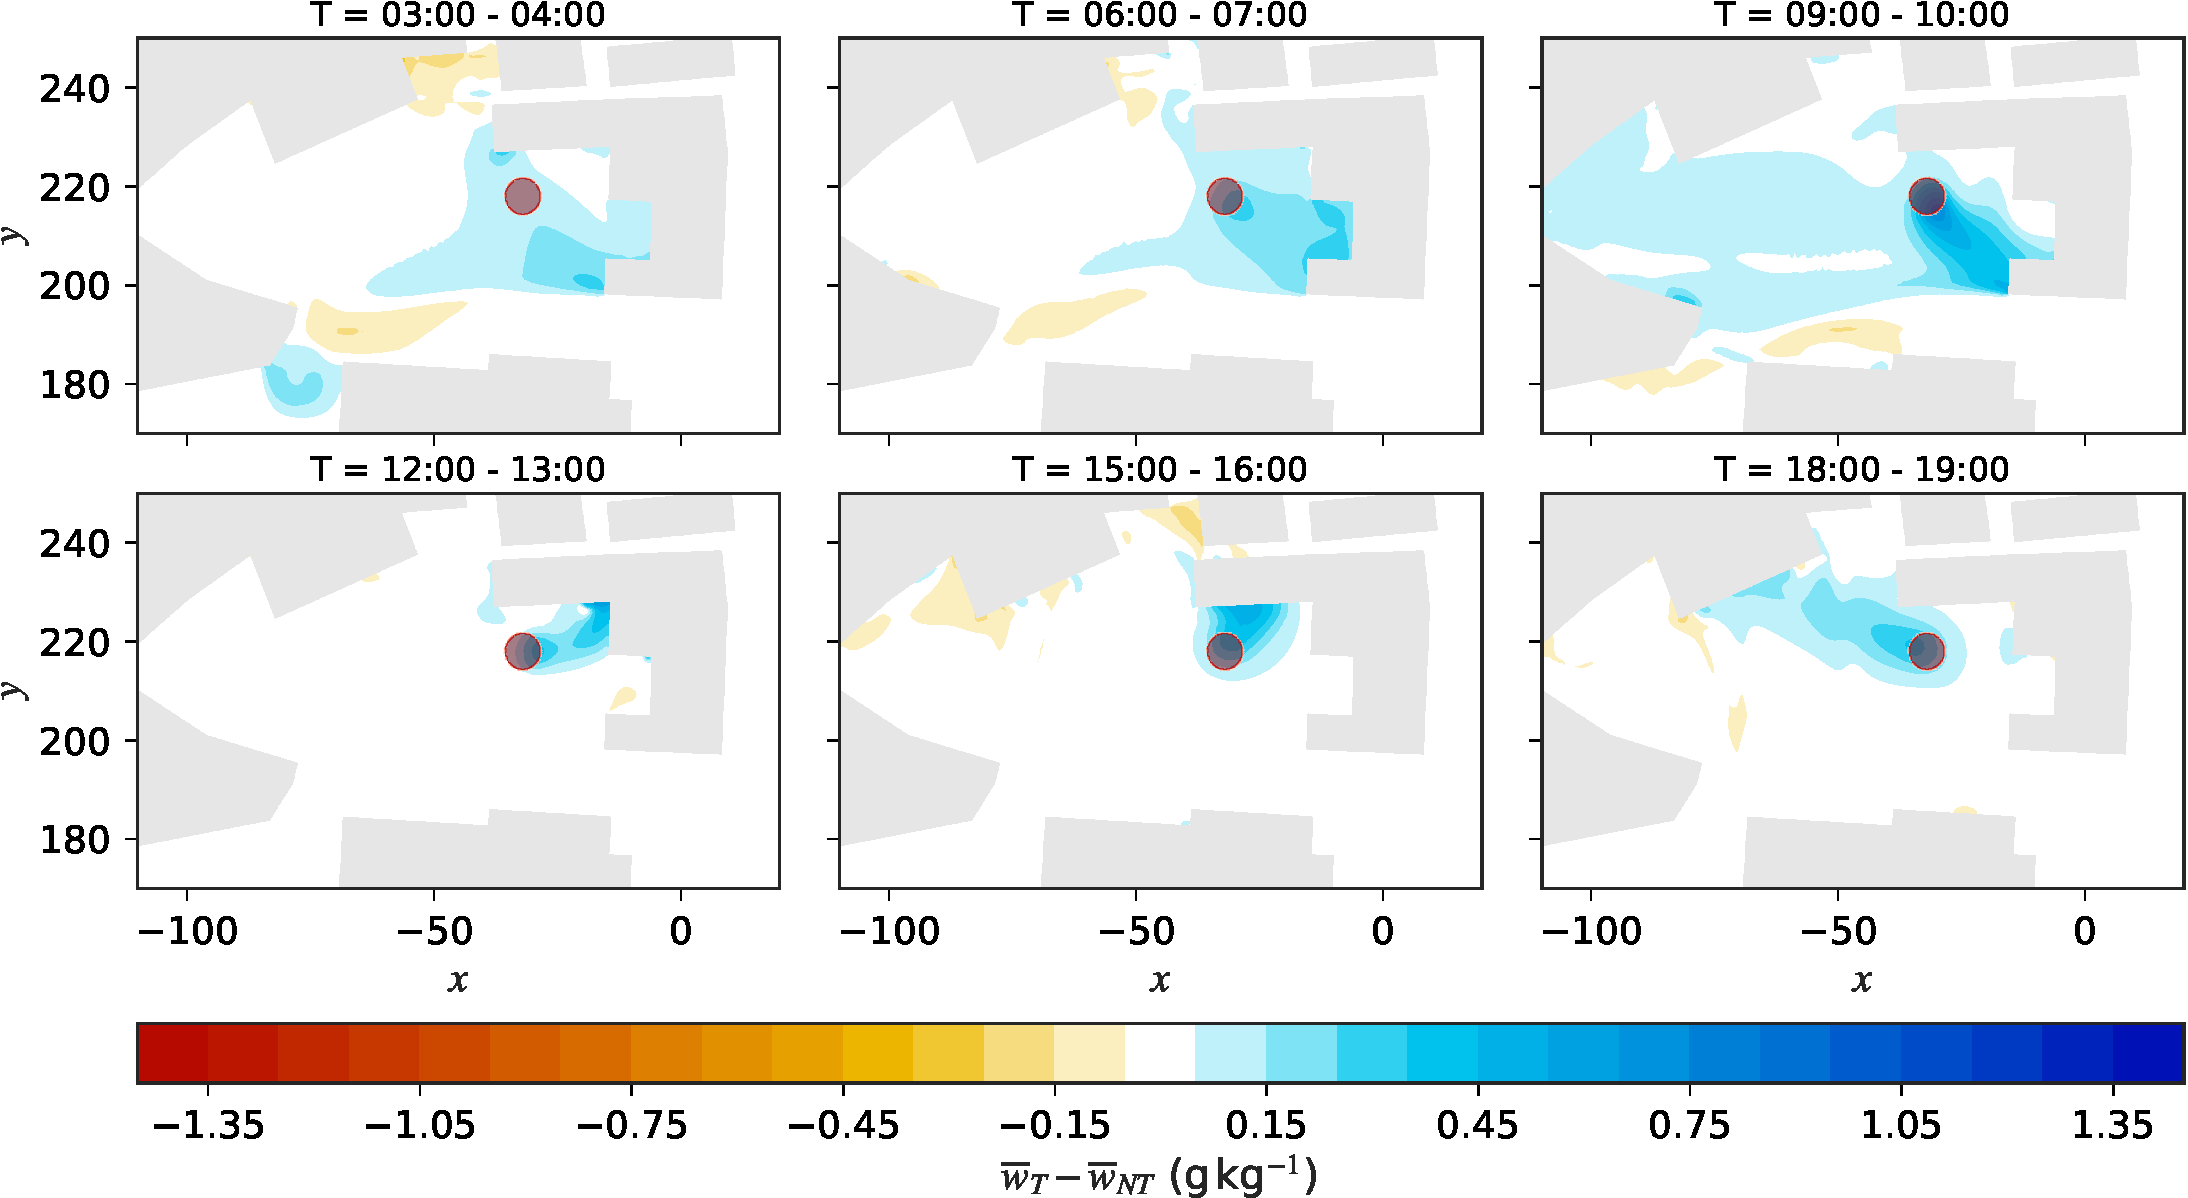
\includegraphics[width=\textwidth]{\figdir/mhof_tree_vs_notree_w_hourlyaveraged_type2-crop.pdf}
	\caption{Hourly-averaged $\overline{w}_{T}-\overline{w}_{\textit{NT}}$ (g\,kg$^{-1}$) at $z=4$ m between 6 different times of the day (03:00 - 04:00, 06:00 - 07:00, 09:00 - 10:00, 12:00 - 13:00, 15:00 - 16:00, and 18:00 - 19:00).}
	\label{fig:wdiff_muensterhof}
\end{figure}


\begin{figure}[p]
	\centering
	\begin{subfigure}[b]{.45\linewidth}
		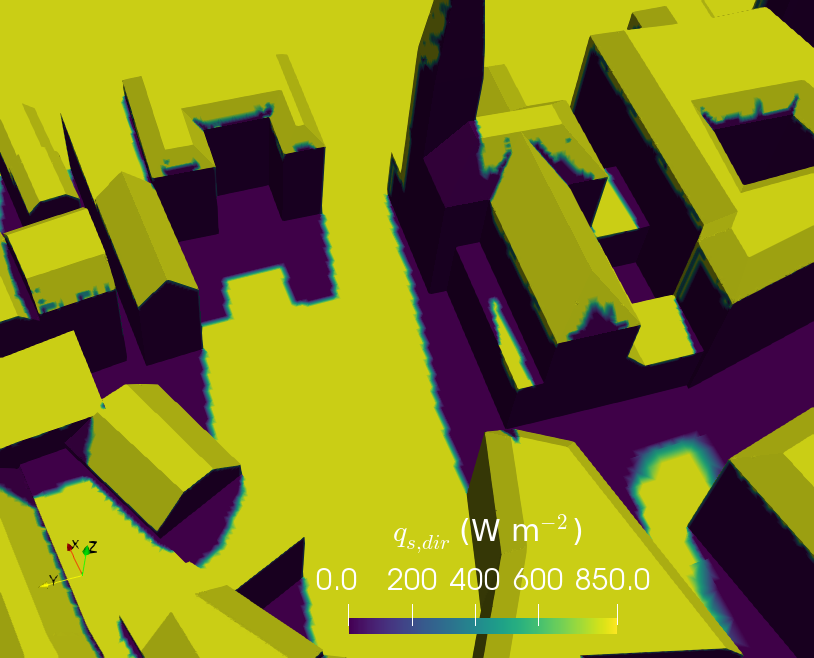
\includegraphics[width=\linewidth]{\figdir/qsdir_basecase_0900.png}
		\caption{$09$:$00$}\label{fig:qrdir_basecase_0900}
	\end{subfigure}\hspace*{\fill}
	\begin{subfigure}[b]{.45\linewidth}
		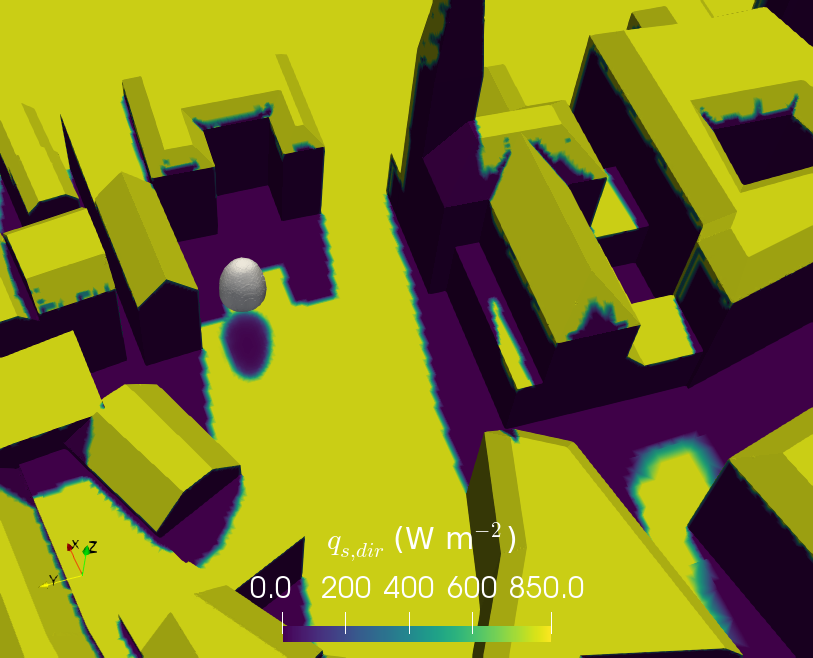
\includegraphics[width=\linewidth]{\figdir/qsdir_tree_0900.png}
		\caption{$09$:$00$}\label{fig:qrdir_tree_0900}
	\end{subfigure}
	
	\medskip
	\begin{subfigure}[b]{.45\linewidth}
		
\includegraphics[width=\linewidth]{\figdir/qsdir_basecase_1200.png}
		\caption{$12$:$00$}\label{fig:qsdir_basecase_1200}
	\end{subfigure}\hspace*{\fill}
	\begin{subfigure}[b]{.45\linewidth}
		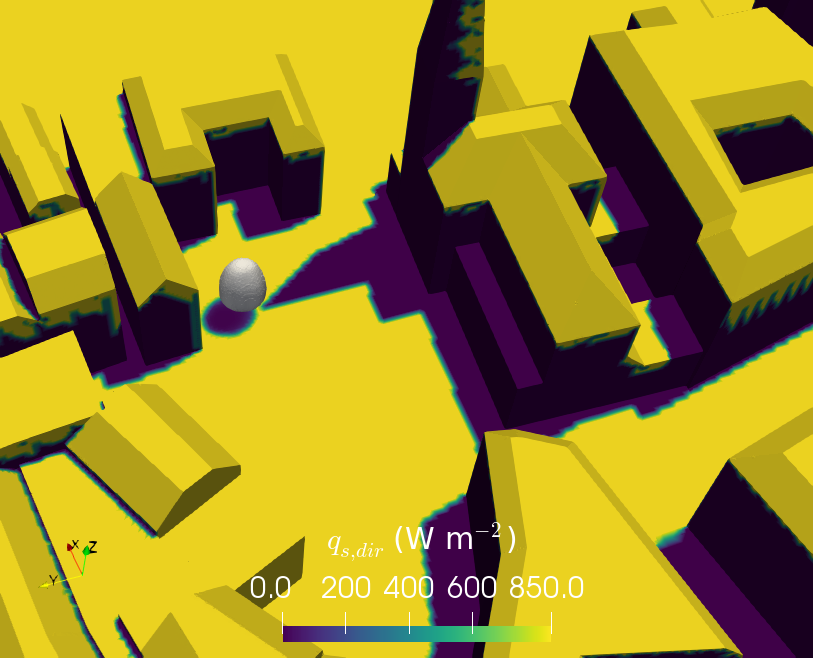
\includegraphics[width=\linewidth]{\figdir/qsdir_tree_1200.png}
		\caption{$12$:$00$}\label{fig:qsdir_tree_1200}
	\end{subfigure}
	
	\medskip
	\begin{subfigure}[b]{.45\linewidth}
		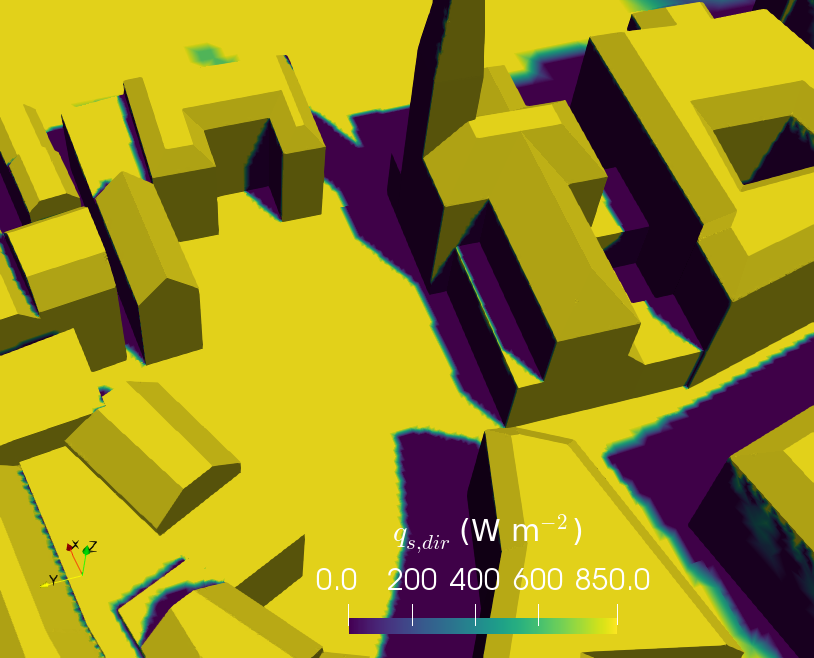
\includegraphics[width=\linewidth]{\figdir/qsdir_basecase_1500.png}
		\caption{$15$:$00$}\label{fig:qsdir_basecase_1500}
	\end{subfigure}\hspace*{\fill}
	\begin{subfigure}[b]{.45\linewidth}
		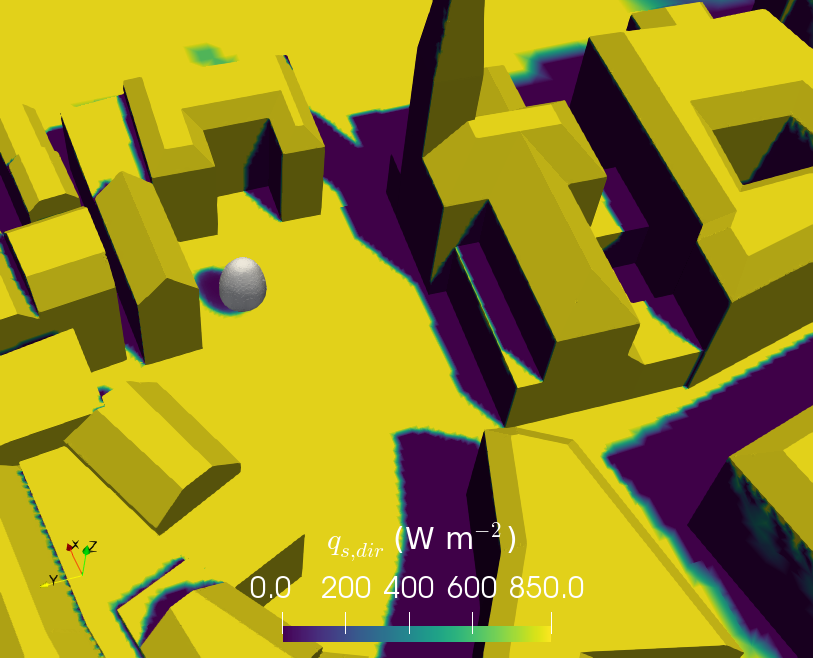
\includegraphics[width=\linewidth]{\figdir/qsdir_tree_1500.png}
		\caption{$15$:$00$}\label{fig:qsdir_tree_1500}
	\end{subfigure}
	
	\caption{Direct short-wave radiation intensity $q_{\textit{s,dir}}$ (W\,m$^{-2}$) arriving at the surface at 3 different time of the day (09:00, 12:00, and 15:00 pm). \subfig{a,c,d} \textit{without} tree and \subfig{b,d,f} \textit{with} tree. The region of tree is indicated by a white surface. }
	\label{fig:qsdir_muensterhof}	
\end{figure}

\begin{figure}[t]
	\centering
	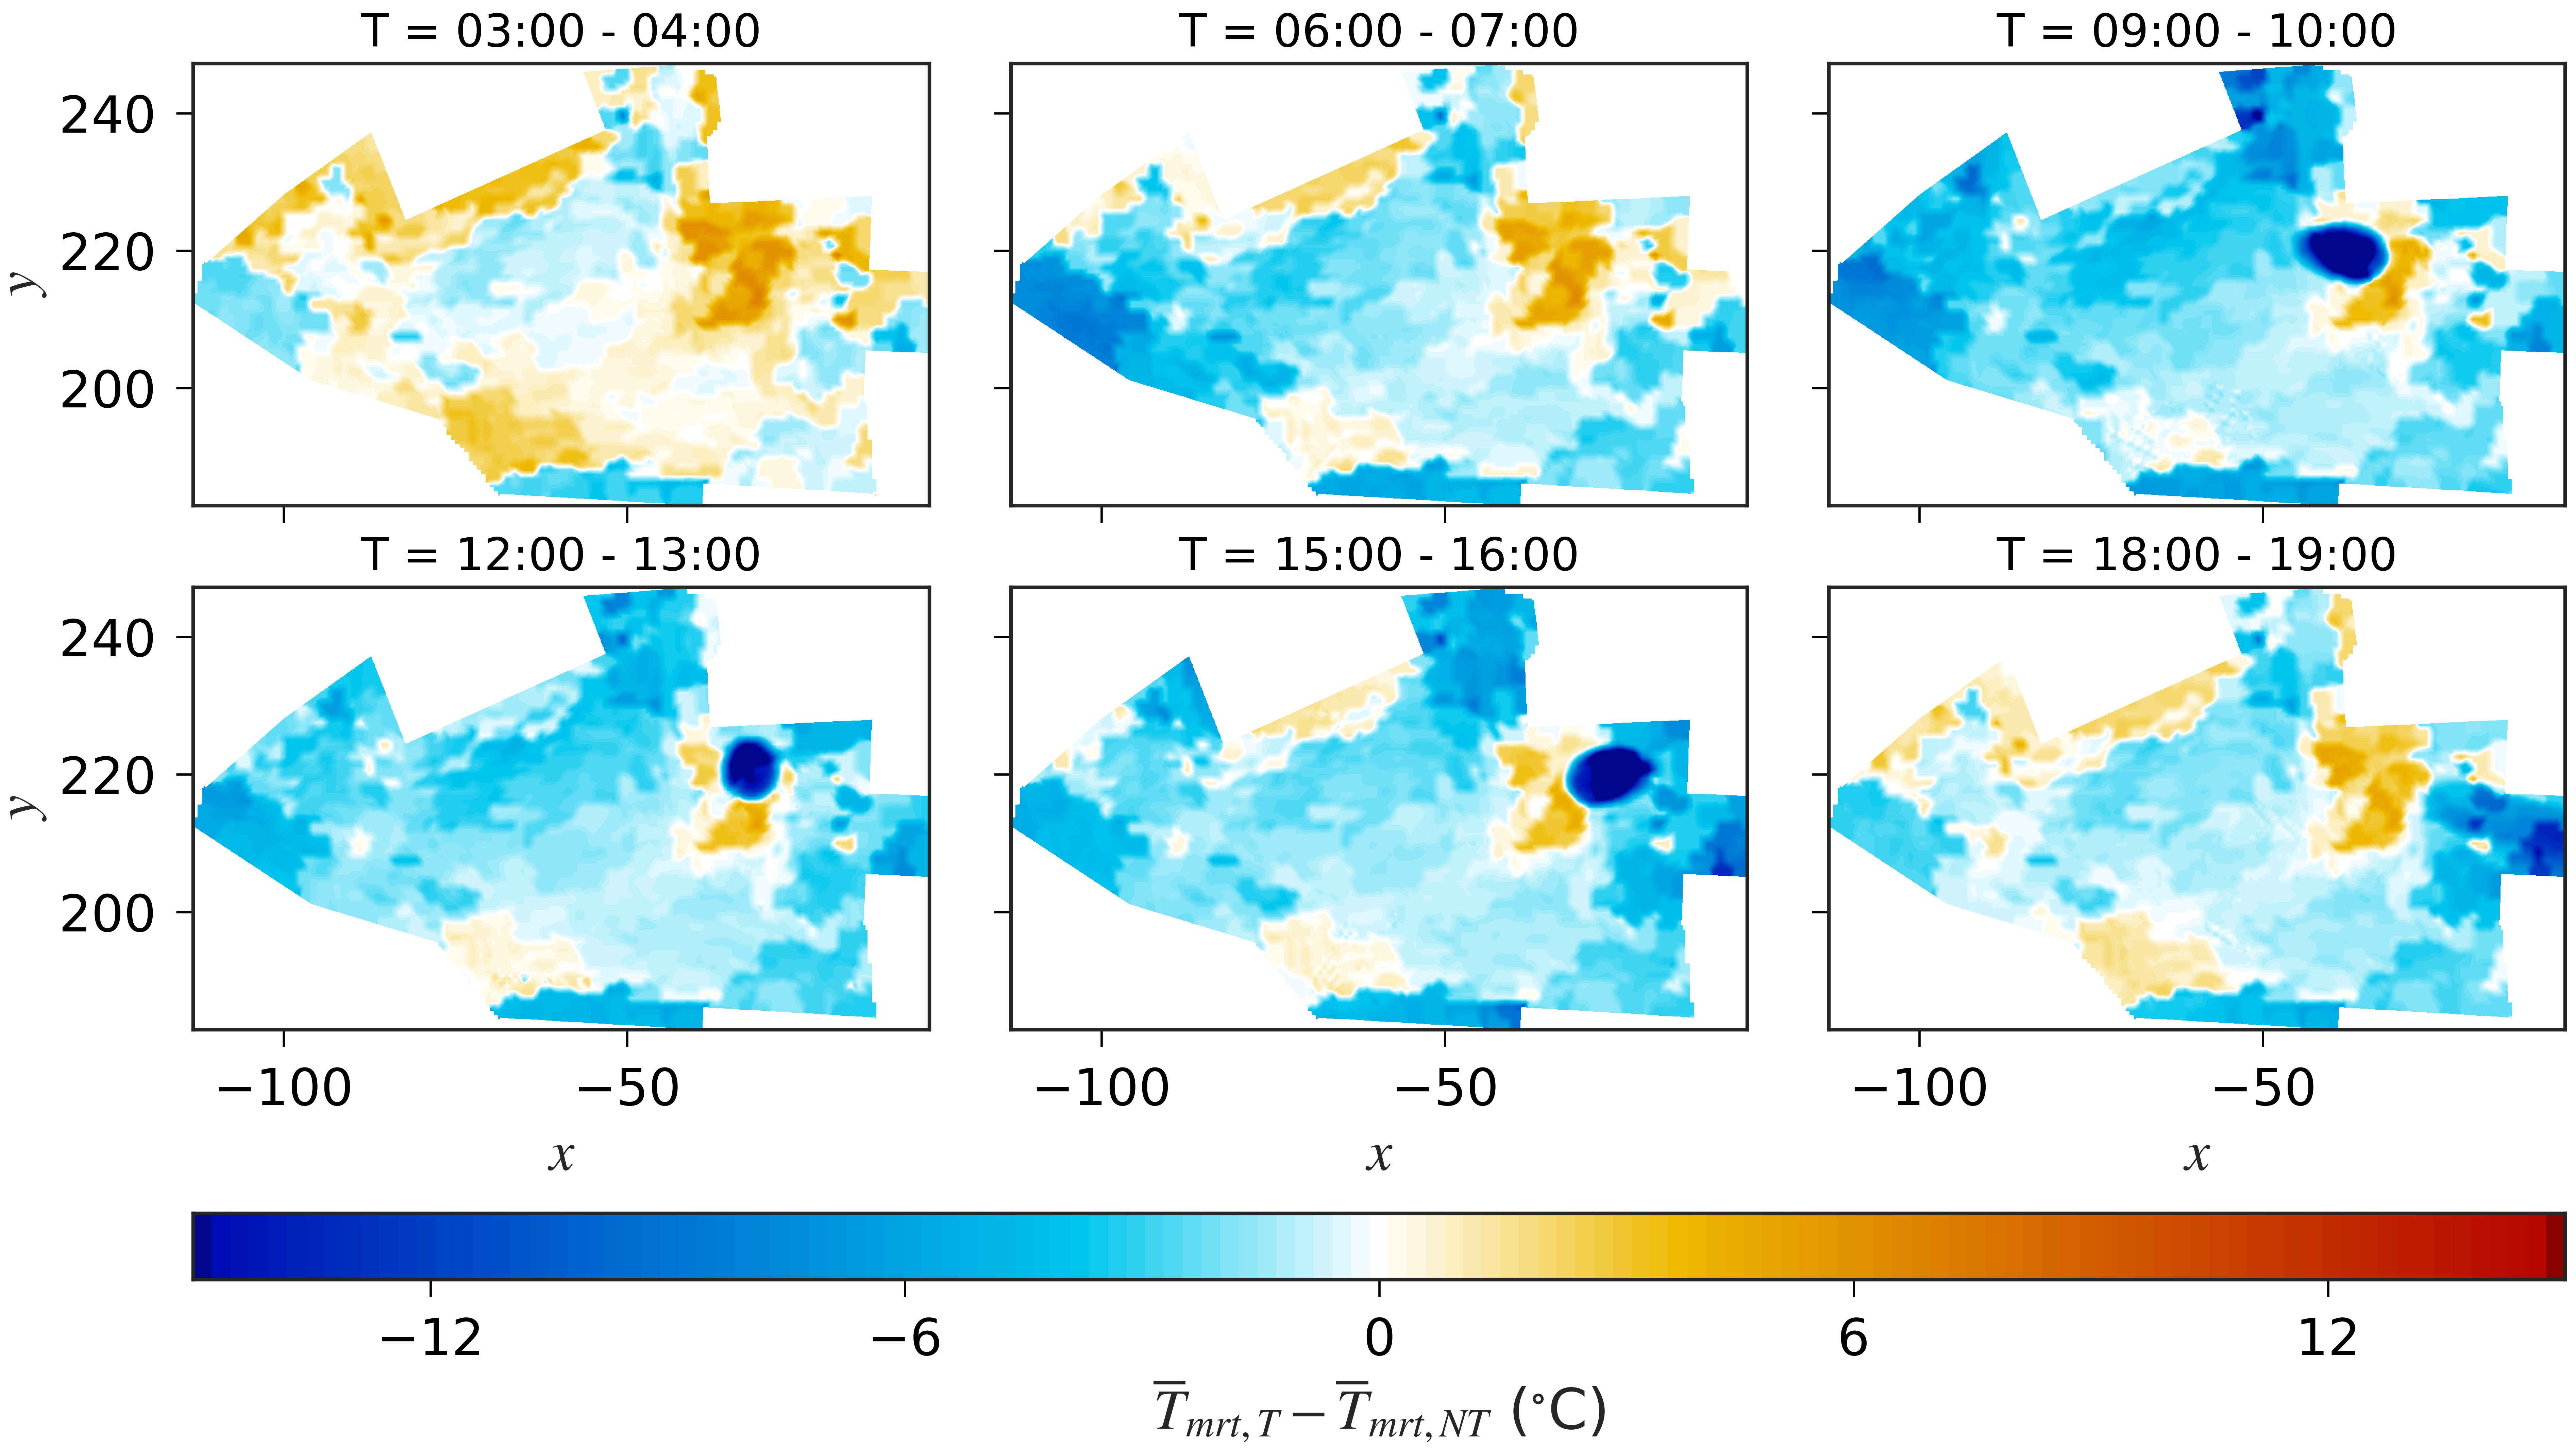
\includegraphics[width=\textwidth]{\figdir/mhof_tree_vs_notree_Tmrt_hourlyaveraged_ground_type2-crop.png}
	\caption{Hourly-averaged $\overline{T}_{\textit{mrt,T}}-\overline{T}_{\textit{mrt,NT}}$ ($^{\circ}$C) at Muensterhof square ground between 6 different times of the day (03:00 - 04:00, 06:00 - 07:00, 09:00 - 10:00, 12:00 - 13:00, 15:00 - 16:00, and 18:00 - 19:00).}
	\label{fig:Tmrtdiff_muensterhof}
\end{figure}

\cref{fig:qsdir_muensterhof} shows direct short-wave radiation intensity $q_{\textit{s,dir}}$ (W\,m$^{-2}$) and the interception of solar radition by the foliage. It is apparent that tree provides shading throughout the day. As we determined in the previous section, solar radiation is an important contributor to mean radiant temperature and the thermal comfort. \cref{fig:Tmrtdiff_muensterhof} shows the mean radiant temperature difference between the cases \textit{with} (T) and \textit{without} (NT) tree $\overline{T}_{\textit{mrt,T}}-\overline{T}_{\textit{mrt,NT}}$ ($^{\circ}$C) of the ground of the Muensterhof square. We see that shading provided by the tree substantially reduces the mean radiation temperature. We see that depending on the solar angle, the location of shading provided by the tree varies in time. However, during night below the foliage, we observe a rise in mean radiant temperature instead. This indicates the radiation trapping at the vicinity of the foliage. Thus, the location of the tree should be optimized to provide the maximum transpirative and cooling due to shading and minimize the negative effect of radiation trapping.

% We see that there is a small drop in the air temperature in the vicinity of the foliage. Furthermore, near-tree building wall temperature is lower, especially at $12$:$00$.
% 
%  Although, it is apparent that the magnitude of temperature change resulted from the tree is much lower than the spatial variability in temperature in the domain. For examples, the eastern exit is seen to convect cool air into the Muensterhof with air temperature lower than the transpirative cooling provided by vegetation.

%% We see that the contribution of a single tree in this domain provides a negligible change in the air temperature. A more interesting question would be the influence of transpirative cooling with a much higher vegetation density in the Muensterhof. The main limitation of such research is whether is it applicable in reality due to design constraints in the square, limited by the regulations.

%	\begin{subfigure}[b]{.45\linewidth}
%		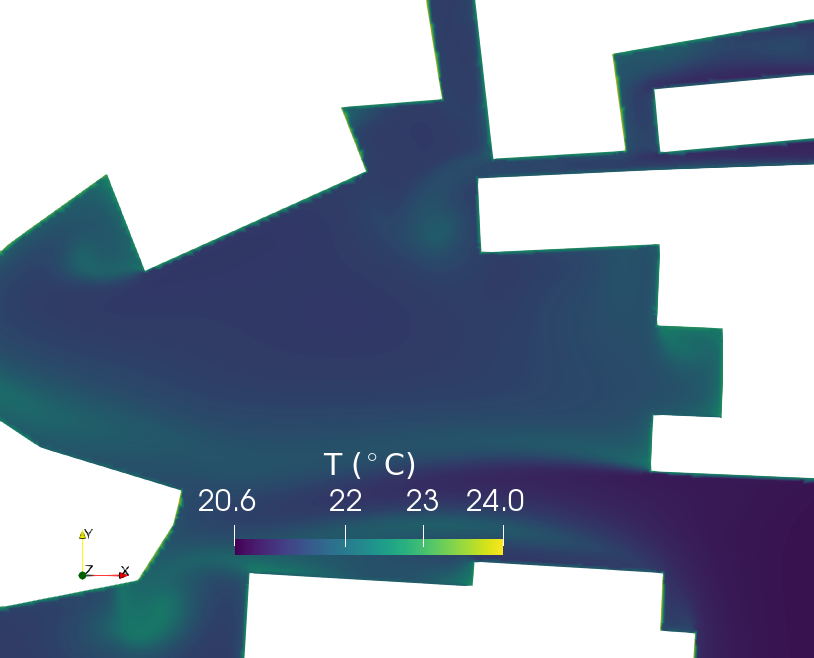
\includegraphics[width=\linewidth]{\figdir/T_basecase_0900.png}
%		\caption{$09$:$00$}\label{fig:T_basecase_0900}
%	\end{subfigure}\hspace*{\fill}
%	\begin{subfigure}[b]{.45\linewidth}
%		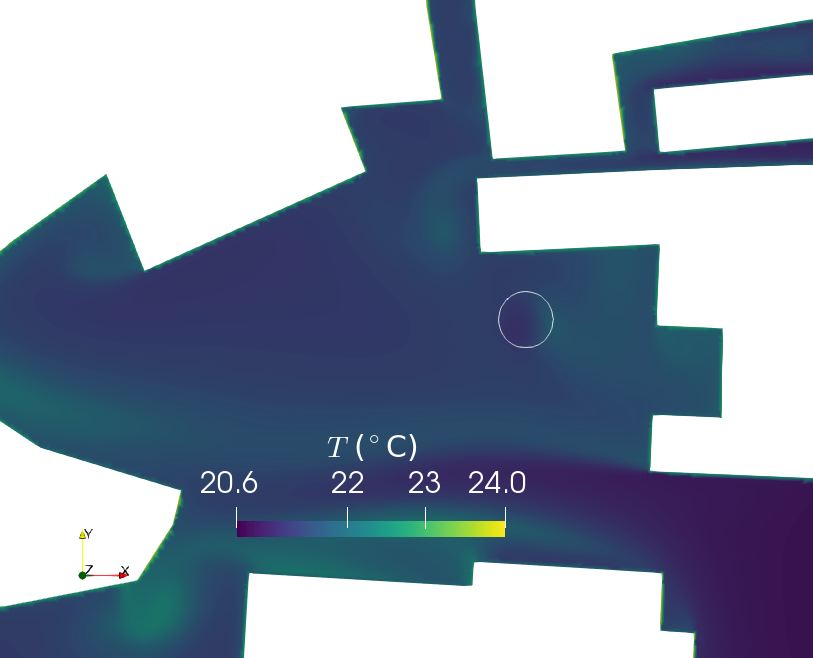
\includegraphics[width=\linewidth]{\figdir/T_tree_0900.png}
%		\caption{$09$:$00$}\label{fig:T_tree_0900}
%	\end{subfigure}
%	\medskip
%	\begin{subfigure}[b]{.45\linewidth}
%	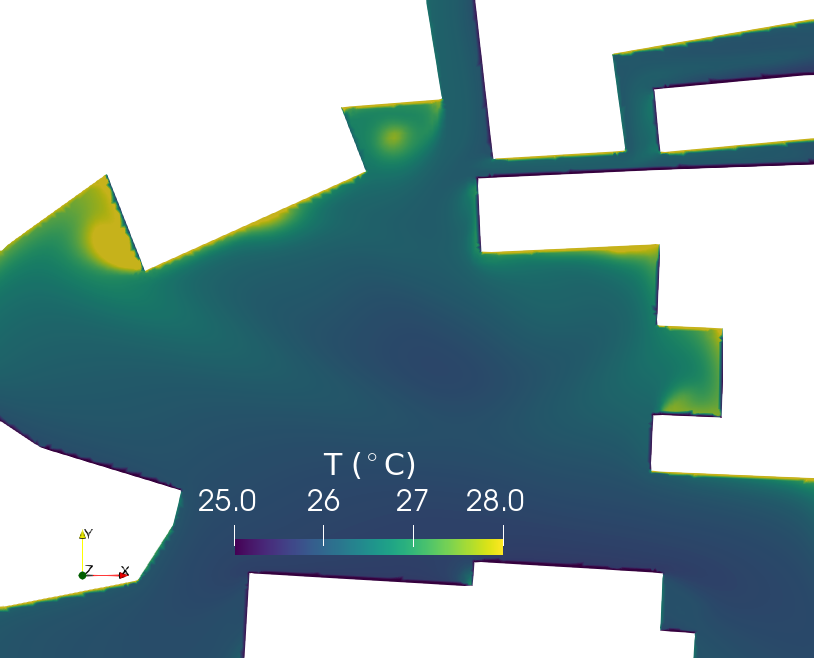
\includegraphics[width=\linewidth]{\figdir/T_basecase_1200.png}
%	\caption{$12$:$00$}\label{fig:T_basecase_1200}
%	\end{subfigure}\hspace*{\fill}
%	\begin{subfigure}[b]{.45\linewidth}
%		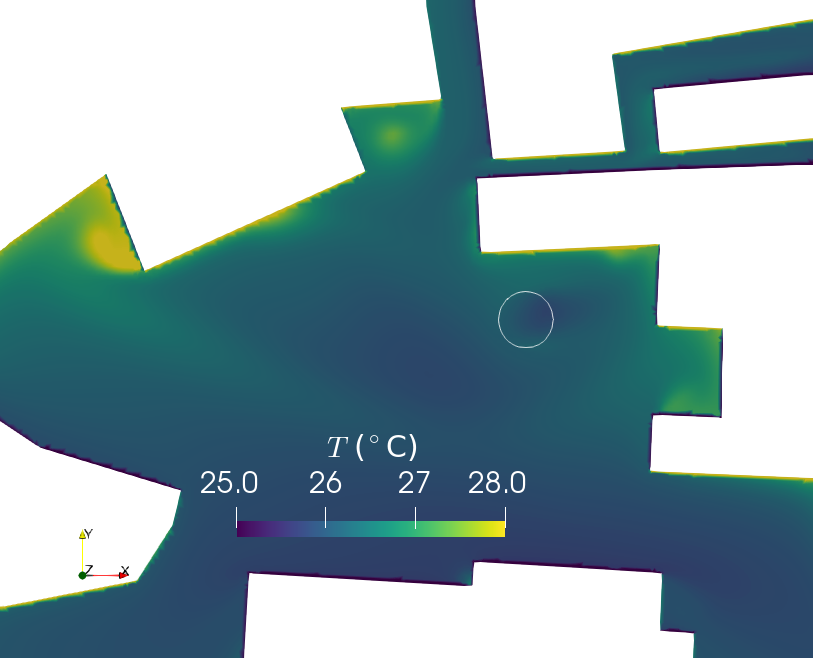
\includegraphics[width=\linewidth]{\figdir/T_tree_1200.png}
%		\caption{$12$:$00$}\label{fig:T_tree_1200}
%	\end{subfigure}
%	\medskip
%	\begin{subfigure}[b]{.45\linewidth}
%		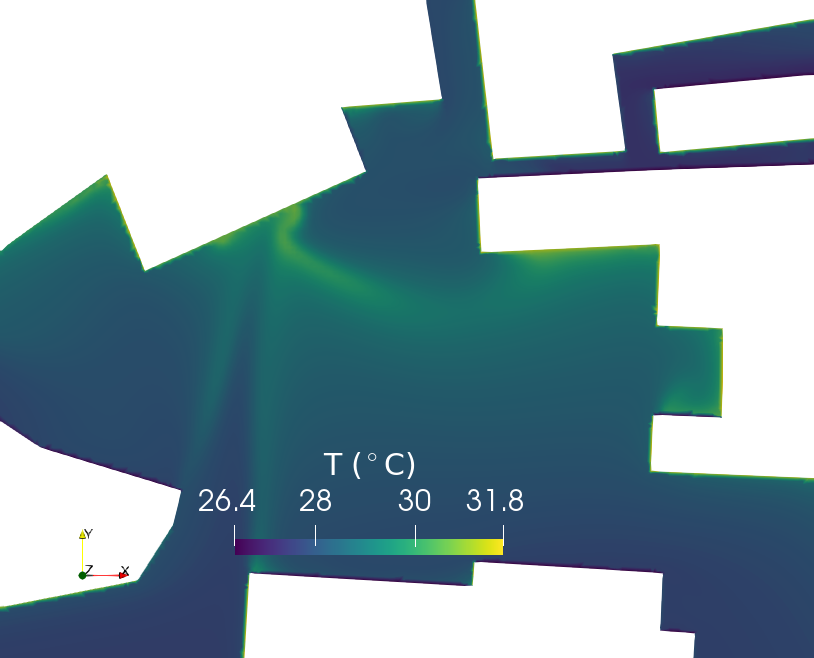
\includegraphics[width=\linewidth]{\figdir/T_basecase_1500.png}
%		\caption{$15$:$00$}\label{fig:T_basecase_1500}
%	\end{subfigure}\hspace*{\fill}
%	\begin{subfigure}[b]{.45\linewidth}
%		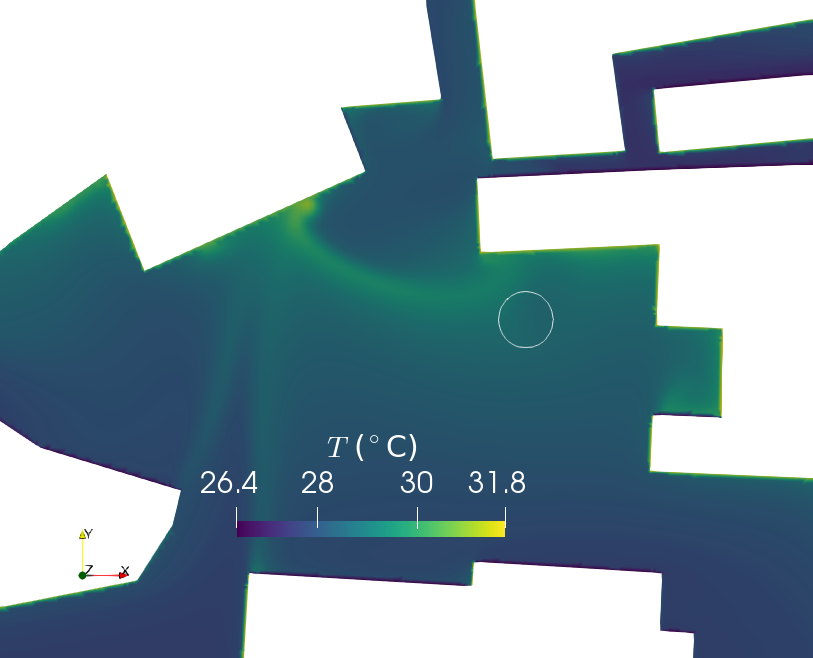
\includegraphics[width=\linewidth]{\figdir/T_tree_1500.png}
%		\caption{$15$:$00$}\label{fig:T_tree_1500}
%	\end{subfigure}



%\begin{figure}[p]
%	\centering
%	\begin{subfigure}[b]{.45\linewidth}
%		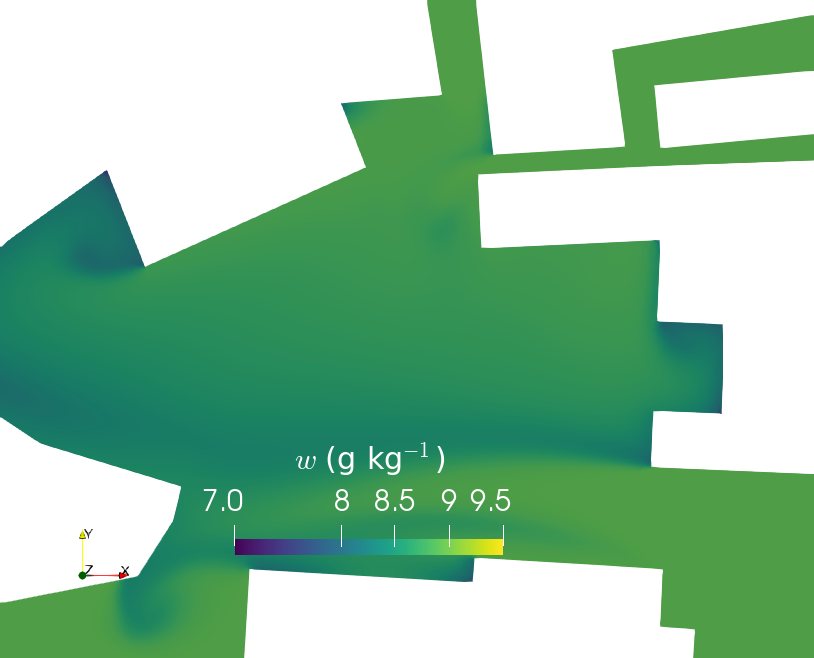
\includegraphics[width=\linewidth]{\figdir/w_basecase_0900.png}
%		\caption{$09$:$00$}\label{fig:w_basecase_0900}
%	\end{subfigure}\hspace*{\fill}
%	\begin{subfigure}[b]{.45\linewidth}
%		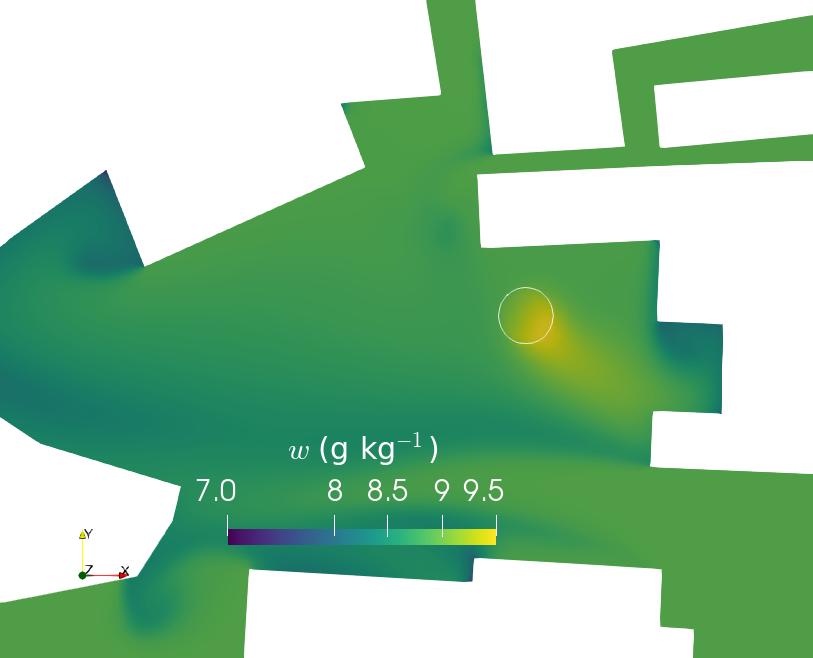
\includegraphics[width=\linewidth]{\figdir/w_tree_0900.png}
%		\caption{$09$:$00$}\label{fig:w_tree_0900}
%	\end{subfigure}
%	
%	\medskip
%	\begin{subfigure}[b]{.45\linewidth}
%		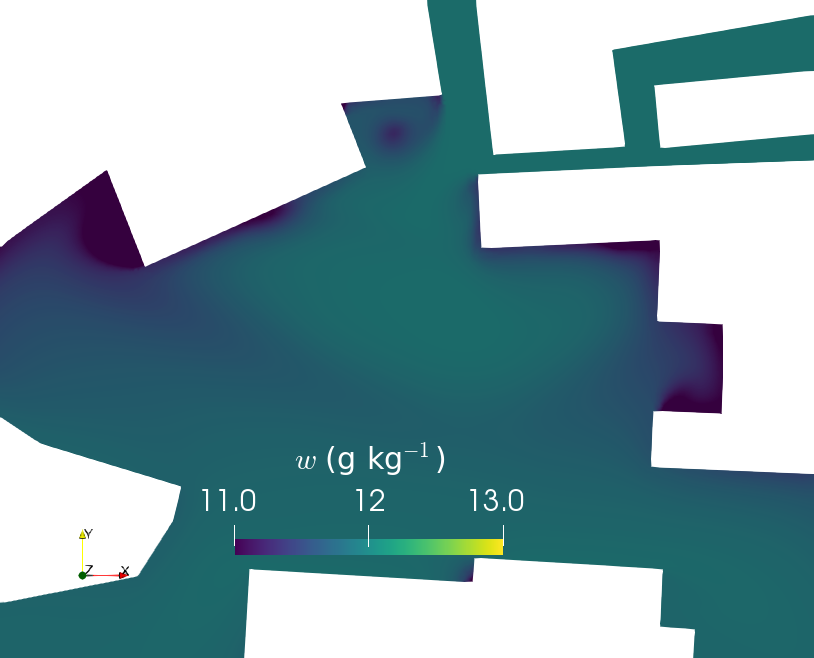
\includegraphics[width=\linewidth]{\figdir/w_basecase_1200.png}
%		\caption{$12$:$00$}\label{fig:w_basecase_1200}
%	\end{subfigure}\hspace*{\fill}
%	\begin{subfigure}[b]{.45\linewidth}
%		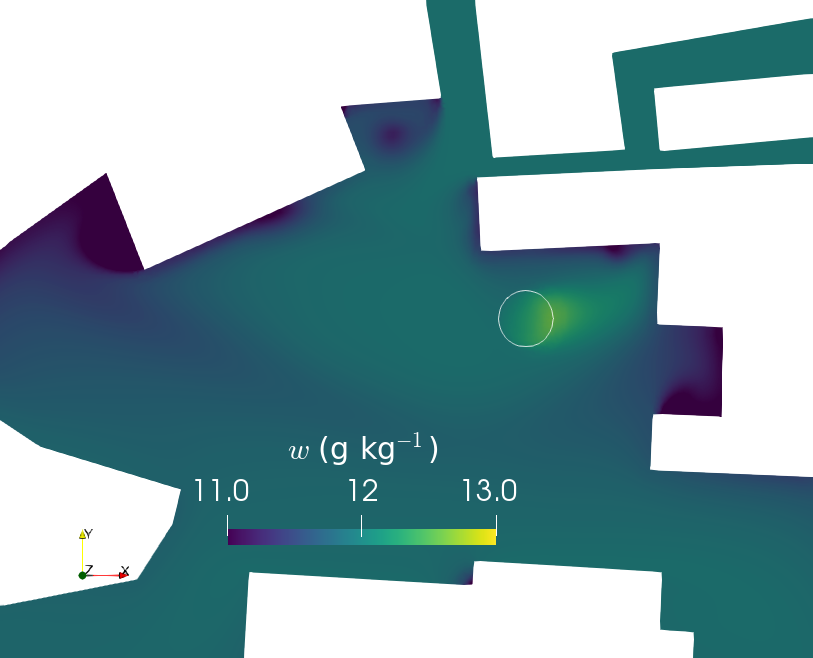
\includegraphics[width=\linewidth]{\figdir/w_tree_1200.png}
%		\caption{$12$:$00$}\label{fig:w_tree_1200}
%	\end{subfigure}
%	
%	\medskip
%	\begin{subfigure}[b]{.45\linewidth}
%		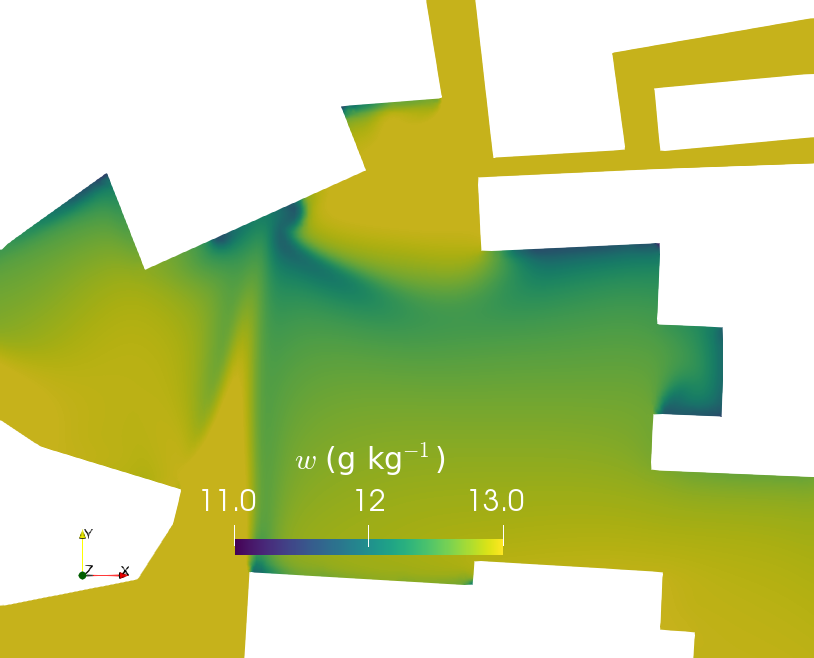
\includegraphics[width=\linewidth]{\figdir/w_basecase_1500.png}
%		\caption{$15$:$00$}\label{fig:w_basecase_1500}
%	\end{subfigure}\hspace*{\fill}
%	\begin{subfigure}[b]{.45\linewidth}
%		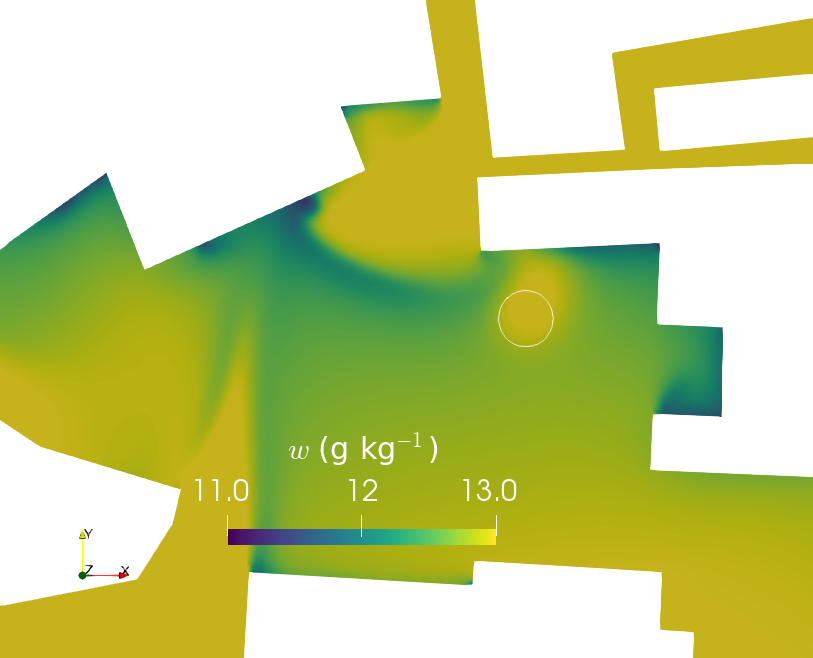
\includegraphics[width=\linewidth]{\figdir/w_tree_1500.png}
%		\caption{$15$:$00$}\label{fig:w_tree_1500}
%	\end{subfigure}
%	
%	\caption{Humidity ratio $w$ (g\,kg$^{-1}$) at $z=4$ m at 3 different time of the day (9 am, 12 pm, and 3 pm). \subfig{a,c,d} \textit{without} tree and \subfig{b,d,f} \textit{with} tree. The region of tree is indicated by a white outline. }
%	\label{fig:w_muensterhof}
%\end{figure}

\newpage

\subsubsection{Multiple tree case}

	\begin{figure}[p]
	\centering
	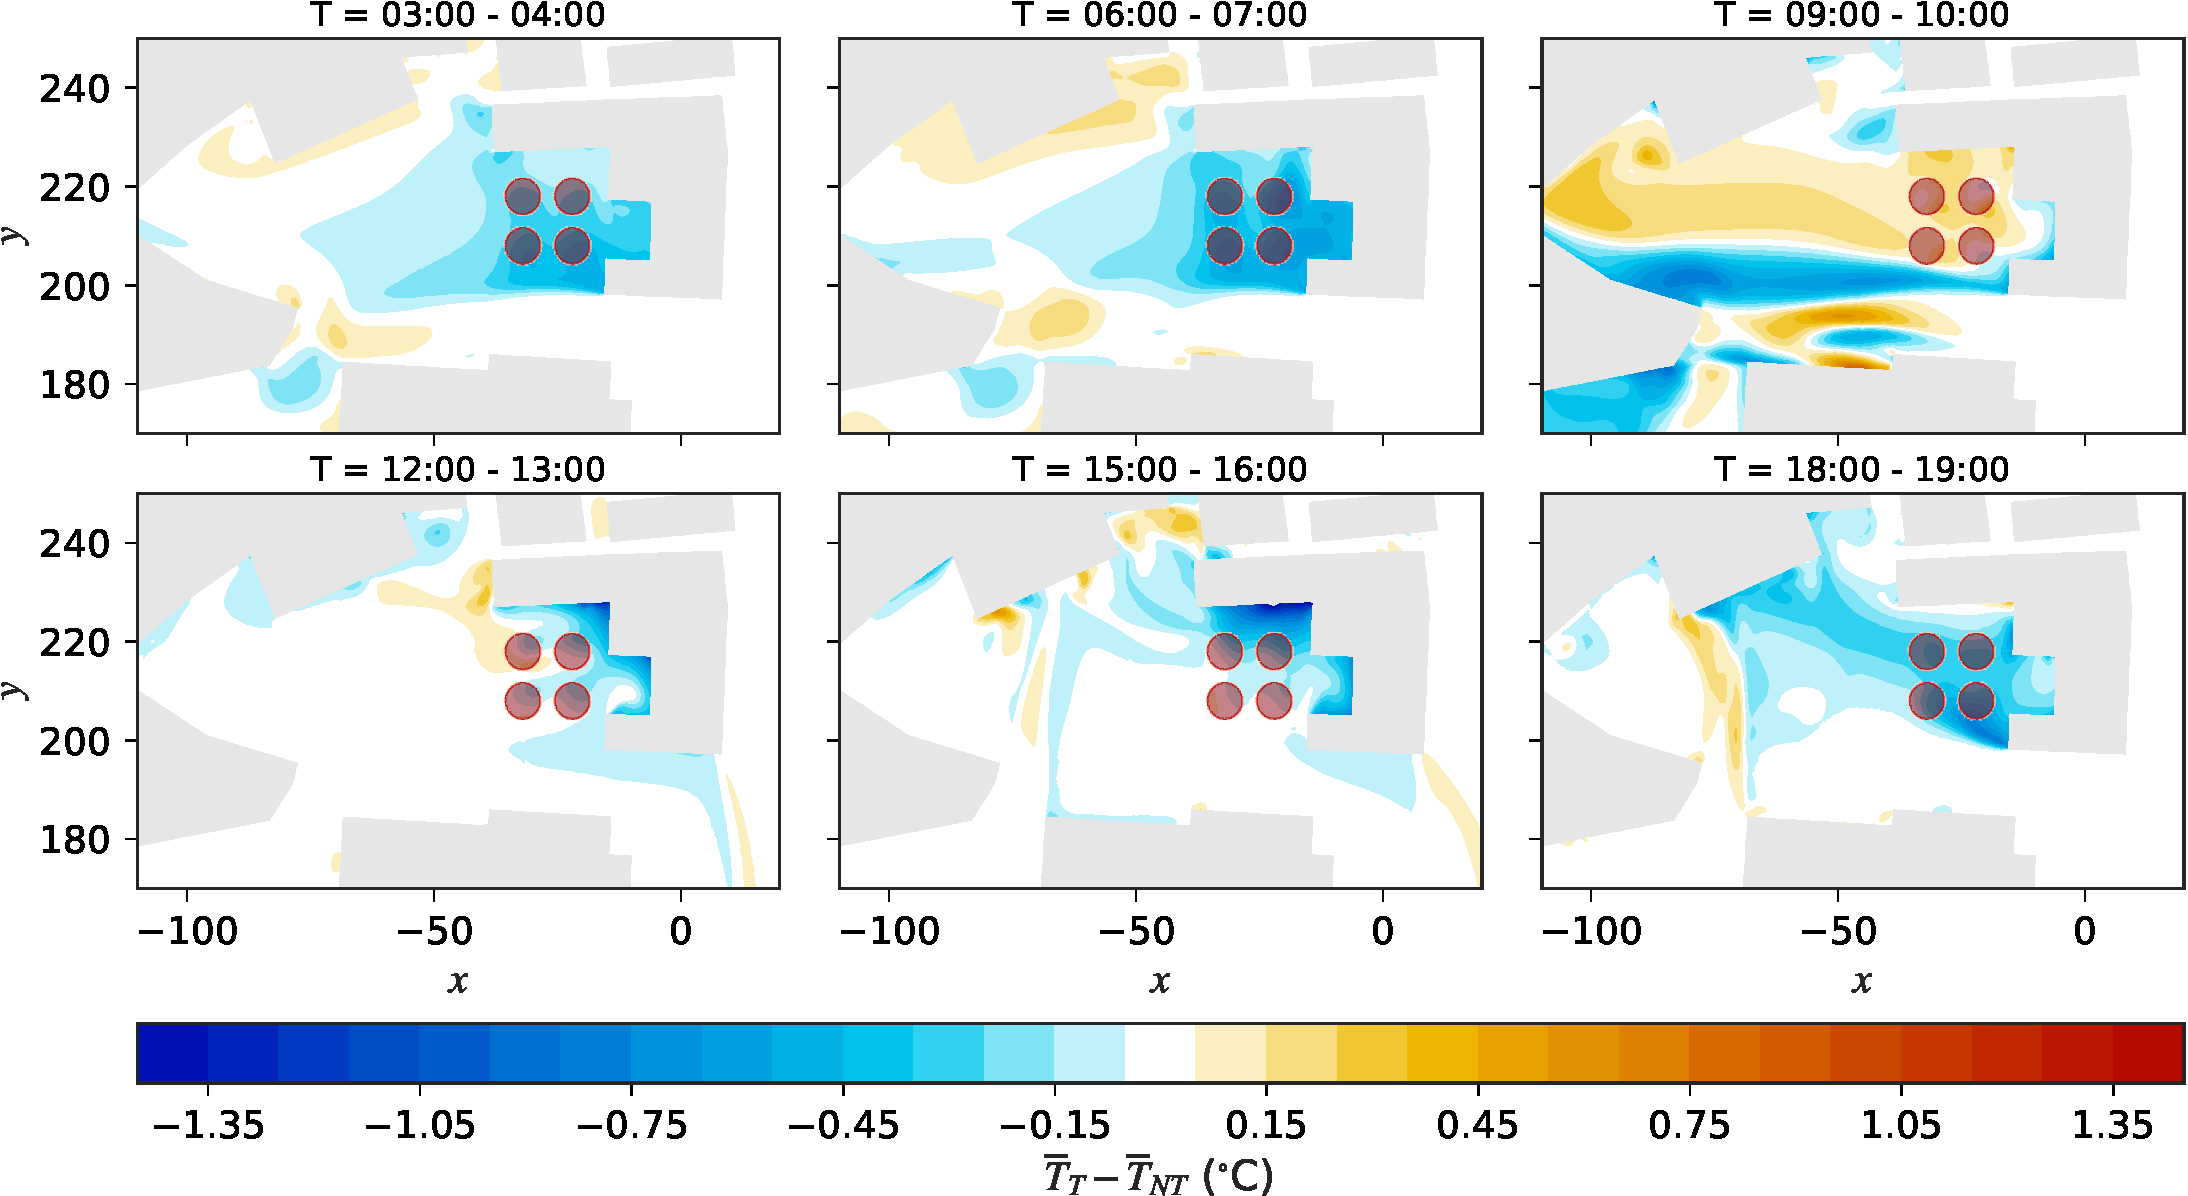
\includegraphics[width=\textwidth]{\figdir/mhof_treegroupA_vs_notree_T_hourlyaveraged-crop.pdf}
	\caption{Hourly-averaged $\overline{T}_{T}-\overline{T}_{\textit{NT}}$ ($^{\circ}$C) at $z=4$ m between 6 different times of the day (03:00 - 04:00, 06:00 - 07:00, 09:00 - 10:00, 12:00 - 13:00, 15:00 - 16:00, and 18:00 - 19:00).}
	\label{fig:mTdiff_muensterhof}
	\end{figure}
	
	\begin{figure}[p]
		\centering
		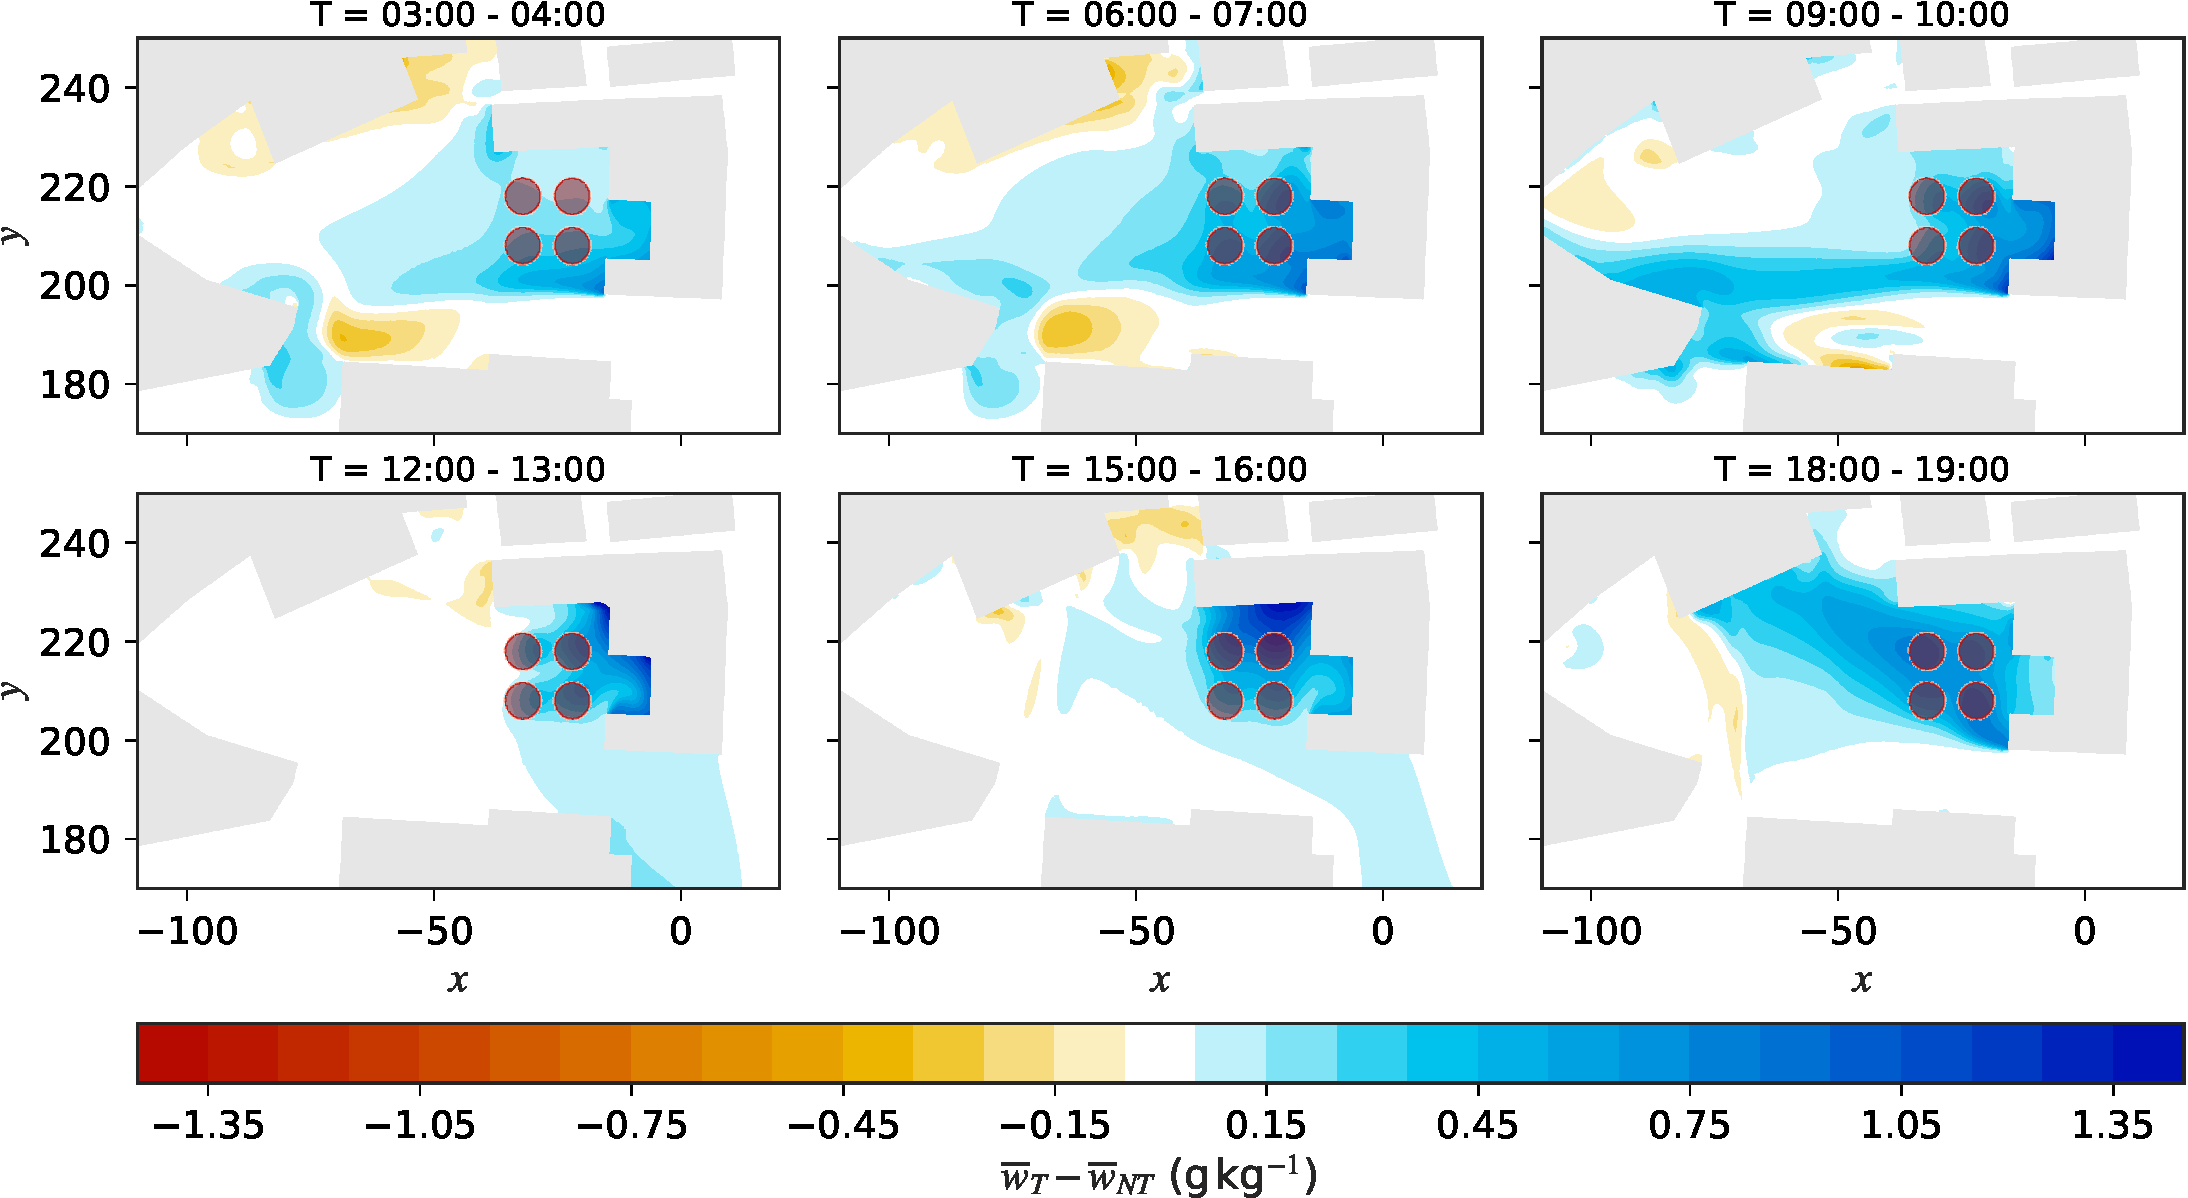
\includegraphics[width=\textwidth]{\figdir/mhof_treegroupA_vs_notree_w_hourlyaveraged-crop.pdf}
		\caption{Hourly-averaged $\overline{w}_{T}-\overline{w}_{\textit{NT}}$ (g\,kg$^{-1}$) at $z=4$ m between 6 different times of the day (03:00 - 04:00, 06:00 - 07:00, 09:00 - 10:00, 12:00 - 13:00, 15:00 - 16:00, and 18:00 - 19:00).}
		\label{fig:mwdiff_muensterhof}
	\end{figure}




To investigate further the influence of vegetation, we study the multiple tree configuration case and compare with the single tree setup. The setup and domain are described in \cref{sec:muenstersetup}. \cref{fig:mTdiff_muensterhof} shows the air temperature difference between \textit{with} and \textit{without} trees. Comparing with the single-tree case configuration (\cref{fig:Tdiff_muensterhof_hourly}), we see a stronger change in air temperature, especially at the walls near the trees. Still, we also see that sometimes (i.e., between 09:00 and 10:00), the average Muensterhof temperature seems to be higher. However, we observe that the cooler regions are more extended than warmer regions. \cref{fig:mwdiff_muensterhof} shows the humidity ratio difference between the cases \textit{with} and \textit{without} trees. The figure shows that humidity inside the square is substantially higher (than compared to \cref{fig:wdiff_muensterhof}) due to the higher density of vegetation, especially near the trees. Due to this, we see that the wall regions near the trees are cooler than in the single tree case.

Furthermore, the study of mean radiant temperature change, \cref{fig:mTmrtdiff_muensterhof}, shows two important aspects of increasing the number of trees. Firstly, we see that below the trees during night, the mean radiant temperature is more positive than with a single tree (see \cref{fig:Tmrtdiff_muensterhof}). This indicates an increased radiation trapping due to higher vegetation density in the area. Secondly, we see that as there are more trees, more areas of the square are cast by shadow, resulting in a larger area with low mean radiation temperature. So, it indicates that more space in the square can provide comfort for the pedestrians. However, due to the location of tree, building and the sun's position, the tree shadow is predominant cast on the nearby buildings instead of the middle of the square where most pedestrians might travel. A better location for trees to cast a shadow would be at the middle of the square. However, due to regulatory constraints (as mentioned in \cref{sec:muenstersetup}), the present location is the only available area of planting trees. We see that, albeit a better site for trees to improve comfort, such regulations finally decide on the feasibility of natural cooling.
	
\begin{figure}[t]
	\centering
	\includegraphics[width=\textwidth]{\figdir/mhof_treegroupA_vs_notree_Tmrt_hourlyaveraged_ground-crop.png}
	\caption{Hourly-averaged $\overline{T}_{\textit{mrt,T}}-\overline{T}_{\textit{mrt,NT}}$ ($^{\circ}$C) at Muensterhof square ground between 6 different times of the day (03:00 - 04:00, 06:00 - 07:00, 09:00 - 10:00, 12:00 - 13:00, 15:00 - 16:00, and 18:00 - 19:00).}
	\label{fig:mTmrtdiff_muensterhof}
\end{figure}


\subsection{Comparison of the cases}

\begin{figure}[t]
	\centering
	\includegraphics[width=\textwidth]{\figdir/mhof_treegroupA_vs_tree_vs_notree_TandTmrt_timeplot_type2-crop.pdf}
	\caption{Diurnal profile comparing three cases: no trees (\textit{None}), single tree (\textit{1 tree}), four trees (\textit{4 trees}): \subfig{a} average air temperature $\langle T\rangle_g$ ($^{\circ}$C), \subfig{b} average mean radiant temperature $\langle \textit{T}_{\textit{mrt}}\rangle_g$ ($^{\circ}$C), \subfig{c} air temperature difference with no tree case, and \subfig{d} mean radiant temperature with no tree case. The values are averaged over the entire Muensterhof square ground.}
	\label{fig:mhofprofile_T_Tmrt}
\end{figure}

In this study, we observe that the multiple tree case provides more cooling of the flow. Comparing \cref{fig:Tdiff_muensterhof_hourly} with \cref{fig:mTdiff_muensterhof}, we see that air temperature is typically lower, especially near the trees. This observation correlates with the humidity ratio of the flow, i.e., \cref{fig:wdiff_muensterhof} and \cref{fig:mwdiff_muensterhof}. This indicates that the increased cooling is most likely due to the increasing transpirative cooling of the flow from the additional trees. To better understand the effect of adding trees in the square, the diurnal variation of the average thermal condition of the Muensterhof ground are compared. The spatial averaging is performed on the surface shown in \cref{fig:mTmrtdiff_muensterhof}. \cref{fig:mhofprofile_T_Tmrt} shows the diurnal variation of the average ground surface temperature $\langle T\rangle_g$ ($^{\circ}$C) and the average mean radiation temperature $\langle \textit{T}_{\textit{mrt}}\rangle_g$ ($^{\circ}$C). It is apparent that adding trees improve (i.e., reduce) the ground surface temperature, as clarified by the difference plot (\cref{fig:mhofprofile_T_Tmrt}c). However, occasionally, the single tree is seen to outperform the multiple tree configuration. It is seen to occur during the morning (between 08:00 and 10:00) and the evening (between 15:00 and 18:00). A direct cause of this observation is not evident. It might be possibly due to the interplay between various environmental conditions such as air temperature, air relative humidity, total shading, soil moisture condition, wind speed, and wind direction. A variation in the flow configuration due to the additional sheltering from the plant or the increased humidity in the air may contribute to the changes in the surface cooling rate and thus the surface temperature. When comparing the mean radiation temperature of the surface (\cref{fig:mhofprofile_T_Tmrt}b and \cref{fig:mhofprofile_T_Tmrt}d), we observe that both cases are very similar to each other, indicating that the shadowing effect of both configurations is similar on the whole Muensterhof ground. Interestingly, it is apparent that during the night, more trees result in a larger rise in the mean radiant temperature. This is indicative of the negative impact of radiation trapping as observed in the previous street-canyon study. However, at daytime, we see the classical benefit of shading as observed in the previous street-canyon study, where maximum reduction in mean radiant temperature was seen to occur during peak solar hours. This implies that, in general, there will be an improvement in the comfort for pedestrians in the Muensterhof square with more trees. In the future, we aim to assess the thermal comfort index (i.e., UTCI) directly inside such complex geometry. Due to computational constraints, it could not be calculated in this study.

\subsection{Conclusion}

The goal of the present study was to demonstrate the application of the developed numerical model in a realistic setup. Muensterhof in Zurich was chosen due to its high interest in urban reforestation by the Zurich city council (DE: Stadrat). The study showed how vegetation modifies the air temperature, humidity ratio and the short-wave radiation inside Muensterhof. We observed several parallels between the academic case of street-canyon and the present case study of real complex configuration. Phenomena observed in complex case such as transpirative cooling effect and the cooling due to shading were also observed in the previous study. In both studies, peak cooling was observed around solar noon when plant transpiration is highest and when the foliage absorbs most solar radiation. The benefit of the academic study was that one could perform a rigorous study on the interplay between various parameters such as soil moisture and the transpirative cooling and assess the influence of water stress on the cooling performance of a plant. However, to understand the true impact of vegetation in reality, cases studies such as in the Muensterhof square was needed. It was seen that the performance of the plant also depends on the flow and building configuration. Even though the trees provide shading throughout the day, the shadowing was seen to depend on the location, its proximity to the buildings, and the path of the sun. Due to the position of the trees, the shading was localized to a sub-region of the Muensterhof square. Though, it must be noted that the location was chosen based on city regulation. The exits of the square and the center of the square are required to be unhindered to enable transit and public event use, respectively. Thus, the city regulation constraints are also vital to accurately assess the impact of vegetation on the climate which cannot be taken into account in academic studies such as the street-canyon case. 

%Therefore, it is seen that, in the future, more detailed studies should be performed to optimize the shadowing providing in the Muensterhof square. It is recommended that focusing on the shading can provide the maximum improvement in thermal comfort. Furthermore, building walls will also have a cooler temperature due to the reduced solar radiation absorption.  

